\documentclass[11pt,a4paper,twoside,openright]{report}

\usepackage[dvips]{graphicx}
\usepackage{xpatch}
\usepackage{tabularx}
\usepackage{subcaption}
\usepackage{enumerate}
\usepackage{times}
\usepackage{float}
\usepackage{afterpage}
\usepackage{amsmath,amssymb,amsthm,mathrsfs,amsfonts,dsfont}    
\usepackage{rotating}  
\usepackage{fancyhdr}
% list without bullets  
\usepackage[inline]{enumitem}  
\usepackage{caption} 
\hyphenation{a-gen-tiz-za-zio-ne}
%\usepackage{csquotes}
\usepackage[round]{natbib}
\usepackage{graphicx}
\usepackage{epstopdf}
\usepackage{tabularx}
\usepackage{booktabs}
\usepackage{hyperref}
\usepackage{afterpage}
\usepackage{amsmath,amssymb}   
\usepackage{rotating}  
\usepackage{fancyhdr}  
\usepackage{enumerate}
\usepackage{wrapfig}
\usepackage{lipsum}
\usepackage{mathtools}
\usepackage{wrapfig}
\usepackage[textsize=tiny]{todonotes}
\usepackage{etoolbox}
\usepackage{algpseudocode}
\usepackage{algorithm}
%%%%%%%%%%%%%%%%%%%%%%% ALGORITHM COMMAND %%%%%%%%%%%%%%%%%
\algrenewcommand\algorithmicrequire{\textbf{Input:}}
\algrenewcommand\algorithmicensure{\textbf{Output:}}

%%%%%%%%%%%%%%%%%%%% END ALGORITHM %%%%%%%%%%%%%%%%%%%
\usepackage{times}
\usepackage{float}
\usepackage{verbatim}
\usepackage{capt-of}
\usepackage{emptypage}
\usepackage{multicol}
\usepackage[acronym]{glossaries}
\usepackage{booktabs}       % professional-quality tables
\AtBeginEnvironment{proof}{\small}
\allowdisplaybreaks[4]
\hyphenation{a-gen-tiz-za-zio-ne}
\hyphenation{pre-sta-zio-ne}
\hyphenation{am-bien-te}
\usepackage{xspace}    
\usepackage[capitalise]{cleveref} %easy references  
% nomenclature
\usepackage{nomencl}  
\makenomenclature    
\renewcommand{\nomname}{Notation}
\renewcommand{\nompreamble}{Column vectors are denoted by bold, lowercase letter (e.g. $\boldsymbol{x}$). The notation  $\boldsymbol{x}^T$ is for row vectors. Matrices are denoted by bold, uppercase letters (e.g. $\boldsymbol{M}$).}

\newcommand{\remps}{$\mathrm{REMPS}$\xspace}
\newcommand{\rempstilde}{$\widetilde{\mathrm{REMPS}}$\xspace}

                                                  
\DeclareRobustCommand{\eg}{e.g.,\@\xspace}                               
\DeclareRobustCommand{\ie}{i.e.,\@\xspace}                              
\DeclareRobustCommand{\wrt}{w.r.t.\@\xspace}                             
\DeclareRobustCommand{\wp}{w.p.\@\xspace}
\DeclareRobustCommand{\quotes}[1]{``#1''}

\DeclareRobustCommand{\remps}{REMPS\@\xspace}
\DeclareRobustCommand{\rempskappa}[1]{$\text{REMPS}_{P,\pi}(#1)$\@\xspace}
\DeclareRobustCommand{\rempskappahat}[1]{$\widetilde{\text{REMPS}}_{P,\pi}(#1)$\@\xspace}
\DeclareRobustCommand{\opt}[1]{$\text{OPT}_{P,\pi}(#1)$\@\xspace}
\DeclareRobustCommand{\opthat}[1]{$\widetilde{\text{OPT}}_{P,\pi}(#1)$\@\xspace}
\DeclareRobustCommand{\dual}[1]{$\text{DUAL}_{P,\pi}(#1)$\@\xspace}
\DeclareRobustCommand{\dualhat}[1]{$\widetilde{\text{DUAL}}_{P,\pi}(#1)$\@\xspace}
\DeclareRobustCommand{\proj}[1]{$\text{PROJ}_{D_{\mathcal{P},\Pi}}(#1)$\@\xspace}
\DeclareRobustCommand{\projhat}[1]{$\widetilde{\text{PROJ}}_{D_{\mathcal{P},\Pi}}(#1)$\@\xspace}
\DeclareRobustCommand{\kl}{D_{\mathrm{KL}}}
\newcommand{\ev}{\mathop{\mathbb{E}}}
\newcommand{\Renyi}{R\'{e}nyi }
\newcommand{\de}{\,\mathrm{d}}
\newcommand{\vtheta}{\mathbr{\theta}}
\newcommand{\vrho}{\mathbr{\rho}}
\newcommand{\vmu}{\mathbr{\mu}}
\newcommand{\vsigma}{\mathbr{\sigma}}
\newcommand{\gradHyJ}{\nabla_{\vrho}J(\vrho)}
\newcommand{\hyscore}[1][\vtheta]{\nabla_{\vrho}\log\nu_{\vrho}(#1)}
\newcommand{\hyscoreprime}[1][\vtheta]{\nabla_{\vrho'}\log\nu_{\vrho'}}
\newcommand{\gradHyJApp}{\widehat{\nabla}_{\vrho}J(\vrho)}
\newcommand{\gradHyJAppPrime}{\widehat{\nabla}_{\vrho'}J(\vrho')}


%\setlength{\paperwidth}{16cm}
%\setlength{\paperheight}{24cm}
%\setlength{\oddsidemargin} {2. cm}
%\setlength{\evensidemargin} {2. cm}
%\addtolength{\oddsidemargin} {-0.4 cm}
%\addtolength{\evensidemargin} {-0.4 cm}
%\linespread{1.1}

\usepackage{geometry}    % Da rivedere
\geometry{
  inner=37.125mm,
  outer=33.4125mm,
  top=37.125mm,
  bottom=37.125mm,
  heightrounded,
  marginparwidth=51pt,
  marginparsep=17pt,
  headsep=24pt,
}
\setlength\parindent{0cm}
\setlength\parskip{1em}
\def\labelitemi{--}

\usepackage[T1]{fontenc}
\usepackage[utf8]{inputenc}
\usepackage[english]{babel}

\renewcommand{\captionfont}{\small}

% definition environment
\newtheorem{definition}{Definition}[section]

\newtheoremstyle{dotless}{}{}{\itshape}{}{\bfseries}{}{ }{}

%% remove dot after theorem title
\theoremstyle{dotless}
% theorem environment
\newtheorem{theorem}{Theorem}[section]

% theorem environment
\newtheorem*{theorem*}{Theorem}

\newtheorem{defi}{Definition}[section]
\newtheorem{prop}{Proposition}[section]
\newtheorem{ass}{Assumption}[section]
\newtheorem{coroll}{Corollary}[section]
\newtheorem{lemma}{Lemma}[section]

% vector norm
\newcommand{\norm}[1]{\left\lVert#1\right\rVert}
\newcommand{\sas}{\int_\mathcal{S} \int_\mathcal{A} \int_\mathcal{S}}
\usepackage{bm}
\newcommand{\mathbr}[1]{\bm{\mathbf{#1}}}
\DeclareMathOperator*{\argmin}{arg\,min}
\DeclareMathOperator*{\argmax}{arg\,max}
\DeclareMathOperator*{\esssup}{ess\,sup}
\pagestyle{empty}

\begin{document}
\thispagestyle{empty}
%\begin{titlepage}
\vspace*{-1.5cm} \bfseries{
\begin{center}
  \large
  POLITECNICO DI MILANO\\
  \normalsize
  SCHOOL OF INDUSTRIAL AND INFORMATION ENGINEERING \\
  Master of Science in Computer Science and Engineering \\
  Department of Electronics, Information and Bioengineering  
  
  \begin{figure}[htbp]
    \begin{center}
      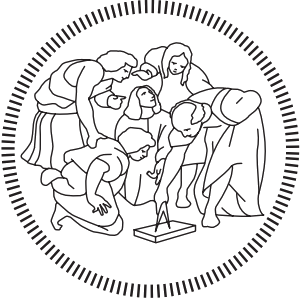
\includegraphics[width=3.5cm]{./pictures/newlogo.png}
 	%
\psfig{file=./pictures/logopm.jpg,width=3.5cm}
    \end{center}
  \end{figure}
  \vspace*{0.3cm} \LARGE



  \textbf{Reinforcement Learning \\ in Configurable Environments: \\ an Information Theoretic approach}\\



  \vspace*{.75truecm} \large
  AI \& R Lab \\
  The Artificial Intelligence and Robotics Lab \\
  Politecnico di Milano
\end{center}
\vspace*{3.0cm} \large
\begin{flushleft}


  Supervisor: Prof. Marcello Restelli \\
  Co-supervisor: Dott. Alberto Maria Metelli
\end{flushleft}
\vspace*{1.0cm}
\begin{flushright}


  Author:\\ Emanuele Ghelfi, 875550 \\ 


\end{flushright}
\vspace*{0.5cm}
\begin{center}



  Academic Year 2017-2018
\end{center} \clearpage
}



\thispagestyle{empty} \normalfont \cleardoublepage
\vspace{17cm}

%\large
\begin{flushright}
\itshape{ A mio padre...}
\end{flushright}

\thispagestyle{empty}  \cleardoublepage
\pagenumbering{Roman}
\newpage
\chapter*{Abstract}

\addcontentsline{toc}{chapter}{Abstract}

The general goal of Reinforcement Learning (RL) is to design agents able to learn a behaviour from interactions with an environment.
Most of the problems tackled by Reinforcement Learning are typically modeled as Markov Decision Processes in which the environment is considered a fixed entity and cannot be controlled. Nevertheless, there exist several real-world examples in which a partial control on the environment can be exercised by the agent itself or by an external supervisor. For instance, in a car race the driver can set up his/her vehicle to better suit his/her needs. With the phrase environment configuration we refer to the activity of altering some environmental parameters to improve the performance of the agent's policy. This scenario has been recently formalized as a Configurable Markov Decision Process (CMDP). \newline
 The aim of this thesis is to further investigate the framework of Configurable Markov Decision Processes. We propose a new information theoretic algorithm, namely Relative Entropy Model Policy Search (REMPS), able to manage CMDPs with continuous action and state spaces. \newline
We propose a theoretical analysis of REMPS deriving the performance gap between the ideal case of the algorithm and the approximated case. Moreover, we empirically evaluate the performance of our approach in three scenarios, showing that it outperforms a naïve gradient method in several situations.

\chapter*{Estratto in Lingua Italiana}
\addcontentsline{toc}{chapter}{Estratto in Lingua Italiana}
L'\textit{Apprendimento per Rinforzo} \citep{sutton_introduction} è un campo dell'\textit{Intelligenza Artificiale} che tratta il problema dell'apprendimento tramite interazione con l'ambiente.
Questa disciplina considera \textit{problemi di decisioni sequenziali}, modellizzati come \textit{Processi Decisionali di Markov} \citep{Puterman:1994:MDP:528623}.
Il decisore, indicato come \textit{agente}, deve stabilire quale azione effettuare considerando l'incertezza dell'ambiente e la sua esperienza. 
Definiamo, in questo contesto, l'apprendimento come processo di adattamento dinamico del comportamento di un agente allo scopo di raggiungere un obiettivo.
Il comportamento dell'agente, che descrive quali azioni prendere in certe situazioni (stati), è chiamato \textit{politica}. Lo scopo degli algoritmi di Apprendimento per Rinforzo è quello di sviluppare agenti in grado di apprendere tramite interazione con l'ambiente, focalizzandosi sull'apprendimento di una politica che massimizzi una metrica di prestazione.
\paragraph{} Nella maggior parte dei problemi affrontati in letteratura, l'ambiente è considerato un'entità fissa, che non può essere controllata. Nonostante questo, esistono diversi esempi reali nei quali può essere esercitato un controllo parziale dell'ambiante dall'agente stesso o da un supervisore esterno. L'ambiente può essere quindi \textit{configurato} per massimizzare la velocità di apprendimento o la prestazione finale dell'agente.
Questo scenario è stato recentemente formalizzato come \textit{Processo Decisionale di Markov Configurabile} \citep{cmdp}. Risolvere un Processo Decisionale di Markov Configurabile significa trovare la politica dell'agente e la configurazione dell'ambiente che, congiuntamente, massimizzino le prestazioni. In \citep{cmdp} gli autori presentano un algoritmo di apprendimento sicuro, \textit{Safe Policy Model Iteration} (SPMI), per risolvere questo tipo di problema. Questo approccio è riuscito a mostrare i vantaggi della configurazione in esempi illustrativi, anche se è ben lungi dall'essere applicabile in scenari reali. Anzitutto, SPMI è applicabile solo a problemi con spazi di stati e azioni finiti, mentre molti esempi interessanti di Processi Decisionali di Markov Configurabili hanno almeno uno spazio di stati continuo. Secondariamente, questo algoritmo richiede una conoscenza esatta della dinamica dell'ambiente. Questa limitazione è rilevante, in quanto in realtà non conosciamo quasi mai la dinamica reale dell'ambiente e, anche se un modello può essere disponibile, questo può essere troppo approssimato o complesso per essere utilizzato (ad esempio il modello fluido-dinamico di una macchina). \newline
\paragraph{} In questa tesi vogliamo investigare più approfonditamente la relazione tra la politica e la configurazione dell'ambiente e trovare tecniche per ottimizzare questi componenti in modo congiunto. Presentiamo un algoritmo, derivato da \textit{Relative Entropy Policy Search} \citep{reps} (REPS), chiamato \textit{Relative Entropy Model Policy Search} (REMPS) che utilizza una formulazione primale-duale per aggiornare i parametri di politica e modello verso un ottimo locale. In aggiunta presentiamo una strategia di proiezione che tiene in considerazione l'effetto congiunto di politica e funzione di transizione. Studiamo le proprietà teoriche del nostro approccio analizzando l'errore dovuto alla differenza di prestazioni dal caso approssimato rispetto al caso ideale. 
La valutazione sperimentale di REMPS è effettuata su tre domini. Il primo dominio, chiamato catena, è semplice e viene utilizzato per visualizzare il comportamento del nostro algoritmo. Il secondo dominio, Cart-Pole, è un banco di prova classico per gli algoritmi di RL. Il terzo dominio, TORCS, è più complesso e mostra le prestazioni del nostro approccio in un problema di guida e configurazione automatica. Nei risultati sperimentali mostriamo che il nostro approccio è migliore rispetto a metodi a gradiente in alcune situazioni.\newline 
\paragraph{} La tesi è strutturata come segue. Il Capitolo \ref{Introduction} presenta il contesto, le motivazioni e lo scopo della tesi. Il Capitolo \ref{chapter2} è un'introduzione all'apprendimento per rinforzo e ai Processi Decisionali di Markov, insieme ad alcune importanti estensioni. Nel Capitolo \ref{chapter3} presentiamo lo Stato dell'Arte dei Processi Decisionali di Markov Configurabili e Relative Entropy Policy Search, siccome il nostro approccio si fonda su queste basi. Nel Capitolo \ref{chapter4} sviluppiamo i contributi principale di questa tesi: l'algoritmo Relative Entropy Model Policy Search e la sua analisi teorica. Nel Capitolo \ref{experimental_evaluation} mostriamo la valutazione sperimentale dell'algoritmo su tre esempi illustrativi. Il Capitolo \ref{capitolo7} contiene la conclusione, nella quale descriviamo brevemente il lavoro svolto e proponiamo possibili estensioni e direzioni di ricerca.
\thispagestyle{empty} \vspace*{.75truecm} \cleardoublepage
\chapter*{Ringraziamenti}

\addcontentsline{toc}{chapter}{Ringraziamenti}

Ringrazio in primo luogo la mia famiglia che mi ha sempre sostenuto sia moralmente che economicamente durante i miei studi. \newline
In secondo luogo desidero ringraziare il prof. Marcello Restelli e il Dott. Alberto Maria Metelli che in questi mesi mi hanno dato tutto il supporto necessario per riuscire a concludere la stesura di questa tesi. A loro sono veramente grato per avermi introdotto al mondo della ricerca e in particolare al mondo del Reinforcement Learning. \newline
Vorrei ringraziare tutti i miei compagni di università, tra questi in particolare Leonardo, Emiliano, Edoardo, Samuele, Giulio. E' anche grazie allo stimolo continuo, alla collaborazione e al confronto che si impara. \newline
Un ringraziamento speciale va alla "Nonna" Luciana per aver allietato le mie giornate di studio con il suo buonissimo ragù. \newline
Un ultimo ringraziamento, ma non di certo per importanza, va alla mia ragazza Giulia per avermi sopportato in questi mesi e per essermi sempre stata vicino.  \newline
\begin{flushright}
Emanuele \\
Milano, 20 Dicembre 2018
\end{flushright}

\thispagestyle{empty} \vspace*{.75truecm} \normalfont \cleardoublepage
\pagestyle{plain}\renewcommand{\chaptermark}[1]{\markboth{\chaptername\ \thechapter.\ #1}{}} 
\renewcommand{\sectionmark}[1]{\markright{\thesection.\ #1}}         
\fancyhead[LE,RO]{\bfseries\thepage}    
                                        
\fancyhead[RE]{\nouppercase{\bfseries\leftmark}}    
\fancyhead[LO]{\nouppercase{\bfseries\rightmark}}     
\renewcommand{\headrulewidth}{0.2pt} 


\nomenclature{$\mathbb{P}(x)$}{Probability of event $x$}
\nomenclature{$s$}{state}
\nomenclature{$a$}{action}
\nomenclature{$r(s,a)$}{reward received after performing action $a$ in state $s$}
\nomenclature{$R(s,a,s')$}{reward received after performing action $a$ in state $s$ and landing in $s'$}
\nomenclature{$\mathcal{S}$}{state space}
\nomenclature{$\mathcal{A}$}{action space}
\nomenclature{$\Delta (\mathcal{X})$}{set of  probability distributions over space $\mathcal{X}$}
\nomenclature{$s_t$}{state at time $t$}
\nomenclature{$t$}{discrete time step $t$}
\nomenclature{$a_t$}{action at time $t$}
\nomenclature{$\Theta$}{family of policy parameters $\Theta \subseteq \mathbb{R}^d$}
\nomenclature{$\boldsymbol{\theta}$}{policy parameter vector $\boldsymbol{\theta} \in \mathbb{R}^d$}
\nomenclature{$\Omega$}{family of model parameters $\Omega \subseteq \mathbb{R}^{d'}$}
\nomenclature{$\boldsymbol{\omega}$}{model parameter vector $\boldsymbol{\omega} \in \mathbb{R}^{d'}$}
\nomenclature{$\pi$}{policy}
\nomenclature{$\Pi$}{policy space}
\nomenclature{$\mathcal{P}$}{configuration space, also referred to as model space}
\nomenclature{$P$}{model configuration, environment dynamics}
\nomenclature{$\pi_{\boldsymbol{\theta}}$}{policy parametrized by $\boldsymbol{\theta}$}
\nomenclature{$P_{\boldsymbol{\omega}}$}{model parametrized by $\boldsymbol{\omega}$}
\nomenclature{$x \sim \mathcal{D}(\cdot)$}{sample $x$ comes from the distribution $\mathcal{D}(\cdot)$}
\nomenclature{$\underset{x \sim \mathcal{D}}{\mathbb{E}} \left[ f(x) \right]$}{Expected value of the function $f$ given that samples $x$ are distributed according to $\mathcal{D}$}
\nomenclature{$G_t$}{Return from time step $t$}
\printnomenclature[0.9in]



%\begin{description}
%\item \textbf{Pr}(x) \tab probability of event x 
%\item s \tab state
%\item a  \tab  action
%\item r   \tab  reward
%\item $\mathcal{S}$    \tab set of all states
%\item $\mathcal{A}$     \tab set of all actions
%\item $\mathcal{R}$     \tab reward function
%\item $\Delta (\mathcal{X}) $   \tab set of  probability distributions over space $ \mathcal{X} $
%\item t \tab discrete time step
%\item$s_t$    \tab state at time t
%\item$a_t$   \tab  action at time t
%\item$\Theta$    \tab family of policy parameters $\Theta = \mathbb{R} ^d$
%\item$\boldsymbol{\theta}$    \tab policy parameter vector $\boldsymbol{\theta} \in \mathbb{R} ^d$
%\item$\Omega$   \tab  family of model parameters $\Omega = \mathbb{R} ^{d'}$ 
%\item$\boldsymbol{\omega}$    \tab model parameter vector $\boldsymbol{\omega} \in \mathbb{R} ^{d'}$
%\item$\pi$    \tab policy
%\item $\mathcal{P}$    \tab model 
%\item$\pi_\theta$    \tab policy parametrized by $\theta$
%\item $\mathcal{P}_\omega$    \tab  model parametrized by $\omega$
%\end{description}


\tableofcontents
\listoffigures
\listoftables
\listofalgorithms
\newpage
\pagenumbering{arabic}
\pagestyle{fancy} \normalfont
% remove footer
\cfoot{}
\chapter{Introduction}
\label{Introduction}
\thispagestyle{empty}

\begin{quotation}
{\footnotesize
\noindent{\emph{Your work is going to fill a large part of your life, and the only way to be truly satisfied is to do what you believe is great work. And the only way to do great work is to love what you do.}
}
\begin{flushright}
Steve Jobs
\end{flushright}
}
\end{quotation}
\vspace{0.5cm}

%% GENERAL FRAMEWORK
Reinforcement Learning \citep{sutton_introduction} (RL) is a field of artificial intelligence (AI) and machine learning (ML) that deals with the problem of learning from interactions. In this context we define learning as the dynamic adaptation process of a behaviour in order to achieve some objective. We, as human beings continually face this problem. For example, as infants we were unable to walk. Nonetheless, we gradually understand the effect of our action through trials and errors, even without a supervisor teaching us how to do it. We start from no knowledge about how our actions influence the world, but in some months we learn how to reach our goal which, in this case, is walking. \newline
Reinforcement Learning lies between the areas of neuroscience, artificial intelligence, optimal control, psychology, operation research and statistics. 
RL considers \textit{Sequential Decision Making problems}, modeled as \textit{Markov Decision Processes} \citep{Puterman:1994:MDP:528623} (MDPs), which are problems arising in many real-world scenarios. In this settings the decision maker, referred to as the \textit{agent}, has to take decisions accounting for the environment uncertainty and its experience.
Agents are \textit{goal-directed}, they need only a notion of goal, a numerical signal to be maximized. Unlike \textit{supervised learning}, in RL there is no need to provide good examples, it is the agent which learns how to map situations to actions. 
The mapping from situation (states) to actions is called \textit{policy} in literature and it represents the agent's behaviour.
Solving an MDP means finding the agent's policy by maximizing the total reward. \newline
The RL approach has proven to be successful in several domains, such as robotics \citep{rl-robotics}, finance \citep{rl-finance}, videogames (Atari, Dota) \citep{rl-atari-1, rl-atari-2, rl-atari-3}, board games (Alpha Go) \citep{alpha-go, alpha-zero}.
%%CMDP
\subsubsection{Motivations}
In most of the problems tackled by RL the environment is considered a \textit{fixed} entity that cannot be controlled. Nevertheless, there exist several real-world examples in which a partial control on the environment can be exercised by the agent itself or by an external \textit{supervisor}. 
With the phrase \textit{environment configuration}, we refer to the activity of altering some environmental parameters to improve the performance of the agent.
Consider, as before, a child learning to walk. His/her parents (supervisors) can dynamically configure the environment, trying to help their child. They can help their child during his/her first steps, they can reduce the pain while falling by using a mat, or they can help their child by setting up goals of increasing difficulty (e.g., walking further). \newline
We can easily notice that most of the existing environments are consist of a \textit{fixed} part and a \textit{configurable} part. For example, in a car race the \textit{fixed} parts are the physics laws, while the \textit{configurable} parts are the wing angle, the type of tyres, the brake settings.
This process of environment configuration is common in many other scenarios (e.g., robotics, e-learning).  \newline
In these examples there is an entity entitled to configuration activity that configures some environment features (transition function, reward, task difficulty) in order to improve the learning speed or the final performance of the agent.
\subsubsection{State of the Art}
The scenarios presented above have been recently formalized as \textit{Configurable Markov Decision Processes} \citep{cmdp} (CMDP). Solving a CMDP means to find the agent's policy $\pi$ together with the environment configuration $P$ which, jointly, maximize the total reward. In  \citep{cmdp}, a safe-learning algorithm, \textit{Safe Policy Model Iteration} (SPMI), is presented to solve the learning problem in the CMDP framework. The basic idea is to optimize a lower bound on the performance improvement so that a monotonic performance improvement is guaranteed. Although this approach succeeded in showing the advantages of configuring the environment in some illustrative examples, it is quite far from being applicable to real-world scenarios. We believe that the most significant limitations of SPMI are two. First, it is only applicable to problems with a finite state-actions space, while the most interesting examples of CMDPs have, at least, continuous state space (e.g., the car configuration problem). Second, it requires full knowledge of the environment dynamics. This latter limitation is the most relevant as, in reality we almost never know the true environment dynamics, and even if a model is available it might be too approximate and hardy usable, being very complex and computationally expansive (e.g., the fluido-dynamical model of a car).
\subsubsection{Goal}
The aim of this thesis is to further investigate the close relationship between policy and environment and to find ways to optimize them jointly in order to achieve high performance.
Our approach is intended to manage CMDPs with continuous action and state spaces and it does not require full knowledge of the model, an approximated (learned) model can be exploited. These features permits the application of our algorithm on real-world cases.
\subsubsection{Contributions}
The contributions of this thesis are algorithmic, theoretical and experimental. We present an algorithm derived from \textit{Relative Entropy Policy Search} (REPS) \citep{reps}, namely \textit{Relative Entropy Model Policy Search} (REMPS), which exploits a primal-dual formulation to update the model and policy parameters toward a local optimum. Moreover, we present a projection strategy suitable for CMDP that takes into account the joint effect of the policy and the transition function. \newline
We derive some theoretical guarantees for the single step of REMPS, obtaining a bound on the difference of performance between the exact case and the approximated case.  \newline
We show the experimental results of our algorithm on some standard RL benchmarks to highlight the importance of configuring the environment.
%%%% OUTLINE
\subsubsection{Thesis Outline}
The structure of this thesis is organized as follows.
In \cref{chapter2} we present the Reinforcement Learning and Markov Decision Processes frameworks, along with some notable extensions. We start from the Markov Decision Process formalization, we introduce the main components such as the transition function, the reward and the policy. Finally we describe the main approaches for solving MDPs, namely Linear Programming, Dynamic Programming and Policy Search. \newline
In \cref{chapter3} we depict the State of the Art of Configurable Markov Decision Processes since our algorithm builds upon them. We focus on the motivations underlying the framework proposal and we outline some limitations of the state of the art method for solving CMDPs. The second part of the chapter is devoted to REPS and its extensions. \newline
In \cref{chapter4} we present the main contributions of this thesis: the REMPS algorithm and its theoretical analysis. In the first part of the chapter we formalize the CMDP learning problem in an information theoretic fashion. Motivated by two theorems we consider three projection strategies suited for CMDPs. The main goal of the theoretical analysis is to provide a finite-sample analysis of the single step of REMPS. \newline
In \cref{experimental_evaluation} we show the experimental evaluations of our algorithm on three illustrative examples. \newline
\cref{capitolo7} contains the conclusion, in which we briefly describe our work together with some possible extensions and research directions. \newline
\cref{LPproof} reports the proof of the Linear Programming solution presented in \cref{sec:lin_prog}.
\cref{gradient_cmdp} contains the extension of two main estimators for the policy gradient to the case of the model gradient. 
In \cref{sec:remps_deriv} we show the derivation of the REMPS solution in closed form.
\chapter{Reinforcement Learning}
\label{chapter2}
\thispagestyle{empty}

\begin{quotation}
{\footnotesize
\noindent{\emph{All models are wrong, but some are useful. \\ 
} }
\begin{flushright}
George E. P. Box
\end{flushright}
}
\end{quotation}
\vspace{0.5cm}

\noindent In this chapter, we present the basics of the Reinforcement Learning framework needed for contextualize the work of the following chapters. We will first introduce the Markov Decision Process model, \cref{sec:MDP}, then we present the main approaches for the \textit{exact} solution of Markov Decision Processes, namely \textit{Linear Programming}, \cref{sec:lin_prog}, and \textit{Dynamic Programming}, \cref{sec:dyn_prog}. In \cref{sec:policy-search} we present \textit{Policy Search} algorithms, that represents an approximate solution to the Markov Decision Processes problem. At the end of this chapter we will consider some notable extensions to the Markov Decision Process framework, \cref{sec:mdp-ext}.
\section{Markov Decision Processes} \label{sec:MDP}
% Informal introduction to MDP
A Markov Decision Process \citep{puterman2014markov} (MDP) is a formal framework for modelling sequential decision making problems. The decision maker is usually called \textit{agent}.
 In MDPs an agent interacts with an \textit{environment} through \textit{actions} and receives a \textit{reward} based on the action and on the current state of the environment. The goal of the agent is to maximize the cumulative sum, possibly discounted, of rewards in a given \textit{horizon} (possibly infinite). The task the agent has to learn is defined through the rewards it receives. 
 \subsection{Formal Model}
 %  Formal introduction to MDP
In this work we consider finite-time MDPs in which time is divided in discrete steps. At each time step $t = 0,1,...,H$ the agent receives a representation $s_t$ of the state of the environment, $s_t \in \mathcal{S}$, takes an action, $a_t \in \mathcal{A}$, receives a reward, $r_t \in \mathbb{R}$, and lands in the next state $s_{t+1}$ according to the environment dynamics $P: \mathcal{S} \times \mathcal{A} \rightarrow \Delta(\mathcal{S})$. Here $H$ denotes the horizon length, $H \in \mathbb{R}^+ \cup \{+\infty \} $.\newline
Formally an MDP is a tuple $\langle\mathcal{S}, \mathcal{A}, R, \gamma, P, \mu\rangle$, where:
\begin{itemize}
\item $\mathcal{S}$ is  the \textit{state space} (discrete or continuous);
\item $\mathcal{A}$ is the \textit{action space}  (discrete or continuous);
\item $R : \mathcal{S} \times \mathcal{A} \times \mathcal{S} \rightarrow \mathbb{R}$ is the \textit{reward function};
\item $\gamma \in [0,1]$ is the \textit{discount factor} for future rewards;
\item $P: \mathcal{S} \times \mathcal{A} \rightarrow \Delta (\mathcal{S})$ is the \textit{transition function}, where $P(\cdot | s, a)$ is the probability distribution over the next states given that the agent executes action $a$ in state $s$;
\item $\mu \in \Delta(\mathcal{S}) $ is the initial state distribution.
\end{itemize}

Formally the reward function is defined over $\mathcal{S} \times \mathcal{A} \times \mathcal{S} $, so a reward realization is \newline $R(s_t,a_t,s_{t+1})$. Usually we forget the dependence on the state $s_{t+1}$ by taking the expectation over the next states according to the environment dynamics:
\begin{equation}
	r(s_t,a_t) = \underset{s_{t+1} \sim P(\cdot | s_t, a_t)}{\mathbb{E}} \left[R(s_t,a_t,s_{t+1})\right] .
\end{equation}
A trajectory is sequence $\tau=\langle s_t, a_t, R_t\rangle_{t=0,...,H}$ in which $s_t$ represent the current state, $a_t$ the action taken, $R_t$ the reward received at time step $t$.
\begin{figure}[tb!]
\centering
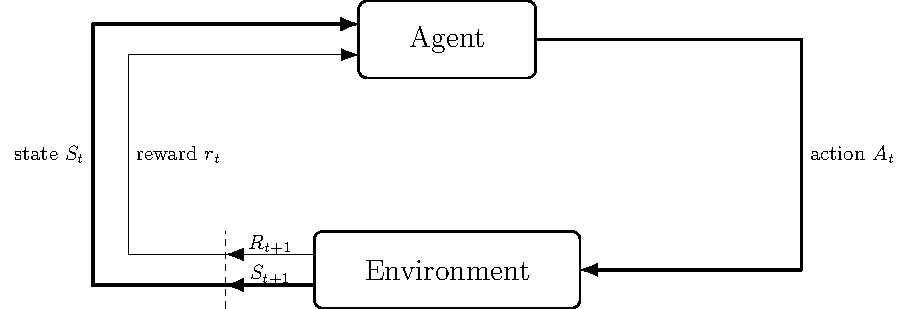
\includegraphics[width=0.8\textwidth]{pictures/agentenv}
\caption{\small Agent Environment interface, from \citep{sutton_introduction}.}
\end{figure}

 \subsection{Transition Model}
 % talk about transition model properties
The transition function must satisfy two properties in order for the problem to be an MDP:
\begin{description}
\item \textit{Markovian}: the current state and action are a sufficient statistic to define the probability over the next states;%Formally the Markovian property states that:
%\begin{equation}
%P(\cdot | s_t, a_t) = P( \cdot | s_t,a_t, s_{t-1}, a_{t-1} ..., s_0, a_0)
%\end{equation}.
\item \textit{Stationarity}: the environment dynamics does not change over time. %, this means that, if $s_{t_1} = s_{t_2}$ and $a_{t_1} = a_{t_2}$, then:
%\begin{equation}
%P(\cdot | s_{t_1}, a_{t_1}) = P( \cdot | s_{t_2},a_{t_2})
%\end{equation}.
\end{description}
These usually are assumptions made in order to simplify the problem. The Markovian property can be ensured by adding enough information to the state. The Stationarity property can be ensured in a similar way, if a task is non stationary it can be translated in a stationary task by adding the time component  to the state description.

 \subsection{Policy} \label{sec:policy}
 % talk about policy properties
The agent interacts with the environment by means of a \textit{policy} that defines its \textit{behaviour}. At each decision epoch a decision maker takes action according to its behaviour $b$. In the most general case the action $a_t$ depends on the whole history from time 0 to time $t$. We denote the set of histories with $\mathbb{H}_t$. A \textit{stochastic} behaviour $b_t$ can be defined as:
\begin{equation}
	b_t : \mathbb{H}_t \rightarrow \Delta(\mathcal{A}) \, .
\end{equation}
A behaviour is said to be \textit{Markovian} if the distribution over actions depends only on the current state:
\begin{equation}
	b_t : \mathcal{S} \rightarrow \Delta(\mathcal{A}) \, .
\end{equation}
A policy is \textit{stationary} if the distribution over actions does not depends on the time.
In this work we will denote a \textit{stationary} \textit{Markovian} policy with $\pi$: 
\begin{equation}
	\pi : \mathcal{S} \rightarrow \Delta (\mathcal{A}) \, .
\end{equation}
It is useful to consider \textit{parameterized} policies, where $\boldsymbol{\theta} \in \mathbb{R}^d$ is the vector of policy parameters. To denote a parameterized policy we use the notation $\pi_{\boldsymbol{\theta}}$ and we omit the subscript when it is clear from the context that the  considered policy is parameterized. The usage of a parameterization implicitly defines a set of policy in which we are interested, we denote the policy family with $\Pi$ and we have $\pi \in \Pi$. 
Common policy parameterizations are:
\begin{description}
\item \textit{Linear} (deterministic), the resulting action is a linear combination of the state features $\phi(s)$:
\begin{equation}
\pi(s) = \boldsymbol{\theta}^T \boldsymbol{\phi}(s) .
\end{equation}
\item \textit{Gaussian}, the resulting action has a gaussian distribution, in which the mean and the variance depend on state features:
\begin{equation}
\pi( \cdot | s) \sim \mathcal{N} ( m( \boldsymbol{\phi}(s)), v(\boldsymbol{\phi}(s)) ) .
\end{equation}
The Gaussian parameterization is useful for continuous action spaces.
\item \textit{Boltzmann}, used for discrete action spaces, the resulting action is a soft-max acting on the weighted state features:
\begin{equation}
\pi(a_i | s) = \frac{e^{\boldsymbol{\theta}_i^T \boldsymbol{\phi}(s)}}{\sum_j e^{\boldsymbol{\theta}_j^T \boldsymbol{\phi}(s)}} \, ,
\end{equation}
where $\boldsymbol{\theta}_i$ is the set of parameters associated to action $a_i$.
\end{description}
In all of these parametrizations the state features might be non-linear features depending on some parameters, e.g. coming from a neural network; radial basis function (RBF) features, tile coding features.

%%%%%%%%%%%%%%%%%% STATE DISTRIBUTION %%%%%%%%%%%%%%%%%%%
\subsection{State distribution} \label{sec:state-distr}
Behaving accordingly to a policy in an MDP induces a distribution over the state space. Here we recall the formulation of the $\gamma$-discounted future state occupancy \citep{pol_grad_func_approx}:
\begin{equation}
	\hat{d}_{\mu,\gamma}^\pi(s) = \sum_{t=0}^{+\infty}\gamma^t \mathbb{P}(s_t = s | \mu, P, \pi) \, .
\end{equation}
The previous formula defines $\hat{d}_\mu^\pi$ of a state $s$ as the sum of the discounted probability of being in $s$ in a time step $t$ given the policy, the initial state distribution and the transition model.
Formally $\hat{d}_\mu^\pi$ is not a distribution as it does not sum up to 1. We normalize it obtaining the $\gamma$ discounted state distribution:
\begin{equation}
	d_{\mu,\gamma}^\pi(s) = (1 - \gamma) \hat{d}_\mu^\pi(s) \, .
\end{equation}
%%%%%%%%%%%%%%%%%% STATE KERNEL %%%%%%%%%%%%%%%%%%%
\subsection{State Kernel}
The transition model and the policy naturally define the \textit{state kernel}, that has a primary role in our work. Formally the state kernel is a function $P^\pi : \mathcal{S} \rightarrow \Delta(\mathcal{S})$. It defines, for each state, a probability measures over the set of states. It consider jointly the effect of the transition model and the policy.
The state kernel is obtained by marginalizing the transition model over the actions:
\begin{equation}
	P^\pi (s' | s) = \int_\mathcal{A} \pi(a | s) P(s' | s, a) \mathrm{d}a \, .
\end{equation}  
%%%%%%%%%%%%%%%%%%%%%%%%%% GOALS and REWARD %%%%%%%%%%%%%%%%%%%
 \subsection{Goal and Rewards}
 % talk about performance objectives, like average reward setting, full return etc
 In Reinforcement Learning the agent's goal is to maximize the total amount of rewards it receives. This is based on the reward hypothesis \citep{sutton_introduction}:
 	
\begin{quotation}
	 \emph{That all of what we mean by goals and purposes can be well thought of as the maximization of the expected value of the cumulative sum of a received scalar signal (called reward).}
\end{quotation}

 Even if a scalar reward signal might seem limiting, this concept has proven to be very flexible and applicable to a wide range of tasks. For example, in locomotion tasks the reward can be defined to be proportional to the amount of distance traveled from the previous step to the current step. In making a robot reaching a goal the reward can be defined as -1 for every step until the agent finds the goal, encouraging the agent to reach the goal as fast as possible.
 It is very important in RL that the reward is given in such a way that it describes what is the goal of the task, it should not describe how to do something. However, in some cases the reward definition might be not trivial. Think for example to a reward for a driving task. In the case of driving it is not trivial to define what does it mean to drive in a good way. \newline
RL tasks can be divided in \textit{episodic} and \textit{continuing}. In episodic tasks we have that $H$, the horizon length, is finite, while in continuing tasks $H = +\infty$.
The \textit{return}, $G_t$ quantifies the agent performance. For \textit{episodic} tasks the return from time step $t$ can be defined as the sum of rewards received until the end of the episode:
\begin{equation}
G_t = \sum_{k=t}^H r_k	\, .
\end{equation}
It is easy to see that for \textit{continuing tasks} this formulation of return diverges since we have an infinite sum of rewards.
To deal with \textit{continuing tasks} we need to introduce the notion of \textit{discounting}. The \textit{discount factor} $\gamma \in [0,1]$ quantifies the present values of future payoffs. 
We introduce the \textit{discounted return} as the cumulative, discounted, sum of rewards until the end of the episode:
\begin{equation}
G_t = \sum_{k=0}^H \gamma^k r_{t+k+1} \, .
\end{equation}
The discount factor, besides having the interpretation mentioned before, can be seen as the probability that the process continues for another step. From the agent point of view, if the discount factor is near to zero greedy actions are profitable since future rewards do not have high values. If the discount factor is near to 1 the agent is \textit{far-sighted}, it is possible for him to sacrifice an action related to a good immediate reward now for a higher reward in the future steps.
We indicate with $G(\tau)$ the return associated with the trajectory $\tau$.
\subsection{Policy and Value Functions}
Policy evaluation is the process of quantifying how good a policy is, it is a key step in almost all RL algorithms. The performance of a policy is defined as the expected value of the return under state and action distribution:
\begin{equation}
J^\pi = \underset{\begin{subarray}{c}
	s_0 \sim \mu \\
	a_t \sim \pi(\cdot | s_t) \\
	s_{t+1} \sim P(\cdot | s_t, a_t)
\end{subarray}
}{\mathbb{E}}\left[ \sum_{t=0}^H \gamma^t R(s_t,a_t, s_{t+1})\right] \, .
\end{equation}
The simple idea formalized above is that policy $\pi_1$ it is better then policy $\pi_2$ if, on average, it collects more rewards. 
Solving an MDP means to find the policy $\pi^*$ such that:
\begin{equation}
\pi^* \in \arg \max_{\pi} J^{\pi} \, .
\label{argmaxJ}
\end{equation}
When we have a parametrized policy we can cast the problem to the point of view of policy parameters. We have that $J$ depends on the policy parameters:
 
\begin{align}
J(\boldsymbol{\theta}) &= \underset{
\begin{subarray}{c}
s_0 \sim \mu \\
	a_t \sim \pi_\theta(\cdot | s_t) \\
	s_{t+1} \sim P(\cdot | s_t, a_t)
\end{subarray}
}{\mathbb{E}}\left[ \sum_{t=0}^H \gamma^{t} R(s_t, a_t, s_{t+1}) \right] . \\
\boldsymbol{\theta}^* & \in \arg \max_{\boldsymbol{\theta}} J(\boldsymbol{\theta}) \, .
\end{align}
The \textit{Value function} (or state-value function) provides a utility measure to a state following a policy. The value of a state $s$ under policy $\pi$, denoted as $v^\pi(s)$, is the expected  discounted return starting from $s$ following the behaviour prescribed by $\pi$:
\begin{equation}
v^\pi(s) = \underset{\pi}{\mathbb{E}} \left[ G_t | s_t = s \right] \, .
\end{equation}
In this way the value function embeds long-term information.
Similarly, we define the value of a state-action pair $(s,a)$ under policy $\pi$ as the expected discounted return starting from $s$, executing action $a$ and following the behaviour $\pi$. This utility measure is denoted as \textit{Q-function} or \textit{action-value function}:
 \begin{equation}
q^\pi(s,a) = \underset{\pi}{\mathbb{E}} \left[ G_t | s_t = s, a_t = a \right] \, .
\end{equation}
 
 The \textit{value function} is not suitable for control as it does not provide information on which action to take. The \textit{Q-function} provides a utility to all actions in a particular state.
 Value function and Q-function are clearly strictly related, the former is obtained by averaging the latter over the action distribution defined by the policy:

 \begin{equation}
v^\pi(s) = \underset{a \sim \pi(\cdot | s)}{\mathbb{E}} \left[ q^\pi(s,a) \right] \, .
\end{equation}

Using the state value function it is possible to re-write the performance of a policy:
\begin{equation}
J^\pi = \underset{s \sim \mu}{\mathbb{E}} \left[ v^\pi(s) \right] \, .
\end{equation}

The value function has also a recursive formulation, denoted as \textit{Bellman expectation operator for $v^\pi$} \citep{Bellman:1957}:
 \begin{equation}
v^\pi(s) = \underset{\begin{subarray}{c}
   a \sim \pi(\cdot | s) \\
   s'\sim P(\cdot | s,a)
   \end{subarray}}
   {\mathbb{E}} \left[R(s,a,s') + \gamma v^\pi (s') \right] \, .
\end{equation}
We can express in a recursive manner also the Q-function, the associated operator is denoted as \textit{Bellman expectation operator for $q^\pi$}:
 \begin{equation}
q^\pi(s,a) = \underset{\begin{subarray}{c}
   a' \sim \pi(\cdot | s') \\
   s' \sim P(\cdot | s,a)
   \end{subarray}}
   {\mathbb{E}} \left[R(s,a,s') + \gamma q^\pi(s',a')\right] \, .
\end{equation}

The Bellman expectation operators have several properties (see \ref{sec:opt-cond}). The operators are mainly used in iterative policy evaluation (see \ref{sec:pi}). We give the formal definition of the Bellman Expectation operators.
%%%%%%%%%%%%%%%%%%% BELLMAN EXPECTATION OPERATOR %%%%%%%%%%%%%%%%%%%%%%
\begin{definition}[Bellman Expectation Operator for $v^\pi$]
	The Bellman expectation operator for $v^\pi$ is defined as $T^{\pi} : \mathbb{R}^{| \mathcal{S} |} \rightarrow \mathbb{R}^{| \mathcal{S} | }$, maps state-value functions to state-value functions:
	\begin{equation}
		(T^{\pi} v)(s) = \underset{\begin{subarray}{c}a \sim \pi(s) \\ s' \sim P(\cdot | s,a) \end{subarray}}{\mathbb{E}} \left[ R(s,a,s') + \gamma v(s') \right] \, .
	\end{equation}
\end{definition} \label{def:bellman_exp_op_for_v}
\begin{definition}[Bellman Expectation Operator for $q^{\pi}$]
	The Bellman expectation operator for $q^{\pi}$ is defined as $T^{\pi} : \mathbb{R}^{| \mathcal{S} | \times | \mathcal{A} |} \rightarrow \mathbb{R}^{| \mathcal{S} | \times | \mathcal{A} |}$, maps Q-functions to Q-functions:
	\begin{equation}
		(T^{\pi} q)(s,a) =\underset{\begin{subarray}{c} a' \sim \pi(s') \\ s' \sim P(\cdot | s,a) \end{subarray}}{
			\mathbb{E}} \left[ R(s,a,s') + \gamma q(s',a') \right] \, .
	\end{equation}
\end{definition} \label{def:bellman_exp_op_for_q}


%%%%%%%%%%%%%%%% OPTIMALITY CONDITIONS %%%%%%%%%%%%%%%%%%5
\subsection{Optimality Conditions}\label{sec:opt-cond}
Besides \cref{argmaxJ} we can define another partial ordering over policies, the ordering induced by \textit{value functions}.
\begin{definition}
\label{optimal_policy}
	Policy $\pi$ is better or equal ($\succeq$) policy $\pi'$ if its expected return is greater or equal to that of $\pi'$ \textit{for all states}:
	\begin{equation}
		\pi \succeq \pi' \iff v^\pi(s) \geq v^{\pi'}(s), \; \forall s \in \mathcal{S} \, .
	\end{equation}
\end{definition}  

Following the previous definition an \textit{optimal policy} is a policy that is better or equal to all other policies in all states. This optimality condition is stricter than the one presented in (\ref{argmaxJ}).
From the definition of optimal policy the \textit{optimal state-value function} and the \textit{optimal Q-function} follows:
\begin{align}
	v^{*}(s) &= \max_\pi v^\pi(s) \\
	q^{*}(s,a) &= \max_\pi q^\pi(s,a) \, .
\end{align}
There is always at least an optimal (deterministic) policy maximizing the state-value function in every state \citep{Puterman:1994:MDP:528623} and all optimal policies share the same \textit{optimal state value-function}. 
The knowledge of the \textit{optimal} Q-function makes it possible to find the \textit{optimal} deterministic policy selecting in every state the action yielding the highest $q$-value: 
\begin{equation}
	\pi^*(s) \in \arg \max_a q^{*}(s,a) \, .
\end{equation}

This holds if we have complete freedom in the selection of the policy (i.e. when $\Pi$ is the set of all Markovian policies). However for practical algorithms we need to restrict our policy space (e.g. parametric policy space), in these cases it is convenient to use the definition of optimal policy in (\ref{argmaxJ}). 
\newline
The optimal state-value function and optimal Q-function satisfy the \textit{Bellman optimality equations}:
\begin{align}
	v^*(s) &= \max_a q^*(s,a) \label{opt_v} \\
		   &= \max_a \underset{s' \sim P(\cdot | s,a)}{
			\mathbb{E}} \left[ R(s,a,s') + \gamma v^*(s') \right] \, . \\			
	q^*(s,a) &= \underset{s' \sim P(\cdot | s,a)}{
			\mathbb{E}} \left[ R(s,a,s') + \gamma \max_{a'} q^*(s',a') \right] \label{opt_q} \, .
\end{align}
At an intuitive level the \textit{Bellman optimality equation} for $v^*$ expresses the fact that the optimal state-value function must equal the expected return for the best action in that state. The \textit{Bellman optimality equation} for $q^*$, similarly, expresses the fact that the optimal Q-function must equal the immediate reward plus the discounted return of the best action in the next state according to the environment dynamic. \newline
The right handside of \cref{opt_v} it's defined as \textit{Bellman Optimality Operator}.

%%%%%%%%%%%%%%%%%%% BELLMAN OPTIMALITY OPERATOR %%%%%%%%%%%%%%%%%%%%%%
\begin{definition}[Bellman Optimality Operator for $v^*$]
	The Bellman optimality operator for $v^*$ is defined as $T^* : \mathbb{R}^{| \mathcal{S} |} \rightarrow \mathbb{R}^{| \mathcal{S} | }$, maps state-value functions to state-value functions:
	\begin{equation}
		(T^* v)(s) = \max_a \underset{s' \sim P(\cdot | s,a)}{\mathbb{E}} \left[ R(s,a,s') + \gamma v(s') \right] \, .
	\end{equation}
\end{definition} \label{def:bellman_opt_op_for_v}
\begin{definition}[Bellman Optimality Operator for $q^*$]
	The Bellman optimality operator for $q^*$ is defined as $T^* : \mathbb{R}^{| \mathcal{S} | \times | \mathcal{A} |} \rightarrow \mathbb{R}^{| \mathcal{S} | \times | \mathcal{A} |}$, maps Q-functions to Q-functions:
	\begin{equation}
		(T^* q)(s,a) =\underset{s' \sim P(\cdot | s,a)}{
			\mathbb{E}} \left[ R(s,a,s') + \gamma \max_{a'} q(s',a') \right] \, .
	\end{equation}
\end{definition} \label{def:bellman_exp_op_for_v}
The Bellman operators (\ref{def:bellman_exp_op_for_v}, \ref{def:bellman_exp_op_for_q}, \ref{def:bellman_opt_op_for_v}, \ref{def:bellman_exp_op_for_q}) are characterized by the following properties, where we will use $T$ to denote both the expectation operator and the optimality operator:
\begin{itemize}
	\item Monotonicity: \begin{equation}
			f_1 \leq f_2 \implies T f_1 \leq T f_2 \, ;
		\end{equation}
	\item Max-Norm contraction:
			\begin{equation}
			\norm{T f_1 - T f_1}_\infty \leq \gamma \norm{f_1 - f_2}_\infty \, , \forall f_1, f_2 \, ;
		\end{equation}
	\item $v^*$ is the \textit{unique fixed point} of $T^*$. $v^\pi$ is the \textit{unique fixed point} of $T^{\pi}$.
	\item Convergence: 
	 \begin{equation}
			\lim_{k \rightarrow \infty} (T^*)^k f = v^* \, , \forall f \in \mathbb{R}^{| \mathcal{S} |} \, 
		\end{equation}
		\begin{equation}
			\lim_{k \rightarrow \infty} (T^{\pi})^k f = v^\pi \, , \forall f \in \mathbb{R}^{| \mathcal{S} |} \, .
		\end{equation}
\end{itemize}
Solving \cref{opt_v} and \cref{opt_q} leads us directly to the MDP solution. Unfortunately these equations are non-linear because of the presence of the $\max$ operator and there is no closed form solution for the general case. 
There exists many iterative solution methods trying to solve an approximation of the Bellman optimality equations that are discussed in the following sections.

\section{Linear Programming} \label{sec:lin_prog}
The problem of computing an optimal policy for an infinite horizon finite-states MDP can be formulated as linear program (LP) \citep{depenoux_probabilistic_1963}. In this section we will go further in the LP formulation since our algorithm extends on this.
The basic idea follows from \cref{optimal_policy}: we want to find the value function maximizing the value of each state weighted by the initial state distribution subject to a feasibility constraint:
\begin{align*}
	\underset{v}{\text{minimize}} & \; \sum_{s \in \mathcal{S}} \mu(s) v(s) \\
	\text{subject to} &  \; v(s) \geq r(s,a) + \gamma \sum_{s' \in \mathcal{S}} P(s' | s,a) v(s') \, , \forall s \in \mathcal{S}, \, \forall a \in \mathcal{A} \, .
\end{align*} 
Where we have $|\mathcal{S}|$ variables and $|\mathcal{S}| |\mathcal{A}|$ constraints. Notice that the maximization role is taken by the constraints, while we need to minimize since otherwise an optimal solution would have infinite values for all variables $v$.
\begin{theorem}[Linear Programming Solution]
$v^*$ is the solution of the above linear program.
\end{theorem} \label{lpth}	


It is possible to prove the above theorem using the properties of the Bellman optimality operators, the interested reader can refer to \cref{LPproof}.
It is also interesting to analyze the Dual Linear Program:

\begin{align*}
	\underset{p}{\text{maximize}} & \; \sum_{s \in \mathcal{S}} \sum_{a \in \mathcal{A}} d(s,a)r(s,a) \\
	\text{subject to} &  \; \sum_{a \in \mathcal{A}} d(s,a) = \mu(s) + \gamma \sum_{s' \in \mathcal{S}} \sum_{a' \in \mathcal{A}} d(s',a') P(s | s', a'), \; \forall s \in \mathcal{S} \\
	& d(s,a) \geq 0, \;  \forall s \in \mathcal{S}, \; \forall a \in \mathcal{S} \, .
\end{align*} 

In the dual program $d(s,a)$ is the discounted state action distribution \citep{pol_grad_func_approx}:
\begin{equation}
	d(s,a) = \sum_t^\infty \gamma^t \mathbb{P}(s_t = s, a_t = a) \, .
\end{equation}

The objective of the dual is the usual objective: maximize the expected discounted sum of rewards.
The constraints are needed for ensuring that $p$ is a valid distribution. 
From the dual program it is possible to extract the optimal policy:
\begin{equation}
	\pi^*(s) \in \arg \max_a d(s,a)\, .
\end{equation}
For each state $s$ we have that $d(s,a^*) = 1$ if action $a^*$ is optimal in state $s$. When there are multiple optimal actions we have a split of the probability between these actions.
The LP formulation is an exact way of solving the MDPs, unfortunately this formulation becomes impractical when the states space grows too much.

\section{Dynamic Programming} \label{sec:dyn_prog}
Dynamic programming \citep{Bellman:1957} (DP) is by far the most common way for solving MDPs when the dynamics and the reward function are known. DP takes into account the sequential or temporal structure of the problem. It is a method for solving complex problems by breaking them into subproblems.
A problem, in order to be solved by DP techniques, must have two properties: \begin{enumerate*} \item Optimal Substructure, \item Overlapping Subproblems \end{enumerate*}. The optimal substructure property means that the principle of optimality applies and the optimal solution can be decomposed into subproblems. The overlapping subproblems property means that subproblems recur many times and the solutions can be stored and reused.
In MDPs both properties are satisfied. The \textbf{Bellman equation} gives the recursive decomposition while the \textbf{state-value function} caches and reuses previous solutions.

\begin{figure}[tb]
\centering
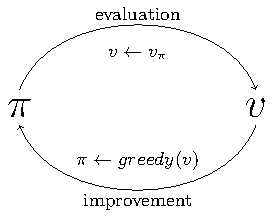
\includegraphics{pictures/value_iteration}
\caption{\small Policy Iteration, from \citep{sutton_introduction}.}
\end{figure}

\subsection{Policy Iteration} \label{sec:pi}
Policy Iteration \citep{howard:dp} is a two stage algorithm: Policy Evaluation (PE) and Policy Improvement (PI).
The first stage (Policy Evaluation) aims at evaluating the current policy through the application of the Bellman Expectation Operator. The PE phase is needed since we want to perform an update of the current policy. The update direction can be computed using the action-value function in the following way. Suppose we know $v^\pi(s')$ for a particular $s'$. To improve the current policy it is enough to compute $q^\pi(s',a)$ for each $a \in \mathcal{A}$ and then to compare it with $v^\pi(s')$. If exists an action $a'$ such that $q(s',a') > v^\pi(s')$, then we can \textit{improve} the current policy using the following update rule:
\begin{equation}
\pi'(s) =
	\left\{
	\begin{array}{ll}
		\pi(s)  & \mbox{if } s \neq s' \\
		\underset{a}{\arg \max} \, q^\pi(s,a) & \mbox{if } s = s'
	\end{array}
\right .
\label{eq:greedy1}
\end{equation}
Basically this update rule states that the new policy is the same as the old policy except for states in which there exists an action $a$ such that the action-value function $q^\pi$ is greater than the value function $v^\pi$. 
The justification for the previous statement comes from the \textit{Policy Improvement Theorem}.
\begin{theorem}[Policy Improvement Theorem]
	Let $\pi$ and $\pi'$ be a pair of policies such that:
	\begin{equation}
		q^\pi(s, \pi'(s)) \geq v^\pi(s) \, , \forall s \in \mathcal{S} \, ,
	\end{equation}
	Then the policy $\pi'$ must be as good or better than $\pi$. 
	\label{th:policy_improvement}
\end{theorem}

Given the previous theorem we can expand the update rule (\ref{eq:greedy1}) by computing the \textit{greedy policy} in all states:
\begin{equation}
\pi'(s) \in \underset{a}{\arg \max} \, q^\pi(s,a) 	\, .
	\label{eq:greedy2}
\end{equation}

This update rule meets the condition of \cref{th:policy_improvement}, so the updated policy is as good as, or better than the old one. 
When the new policy is as good as the old, $v^{\pi'} = v^\pi$, we know, thanks to the optimality operator property, that $v^\pi = v^*$, we have obtained the optimal policy.
Now we can formalize the Policy Iteration Algorithm, see \cref{alg:policy-iteration}.
All the previous ideas can be easily extended to the case of stochastic policies.

\begin{algorithm}[tb]
  \caption{Policy Iteration
    \label{alg:policy-iteration}}
  \begin{algorithmic}[1]
  \Require{$\mathcal{S}, \mathcal{A}, P, R$}
  \Ensure{$\pi \approx \pi^*$}
  \State Initialize $v^\pi$ and $\pi$ randomly
  \Repeat
  \State $v^\pi$ $\leftarrow$ Evaluate policy $\pi$ by applying $T^{\pi}$
  \State $\pi$ $\leftarrow$  Improve policy $\pi$
  \Until{no improvement found} \\
  \Return{Policy $\pi$} 	
  \end{algorithmic}
\end{algorithm}

\subsection{Value Iteration}  
The Value Iteration (VI) algorithm performs evaluation and improvement in the same step. While Policy Iteration performs a search in the space of policies, Value Iteration searches in the space of value functions, calculating the policy only in the last step.
Value Iteration is obtained simply by turning the Bellman Optimality Operator into an update rule:
\begin{equation}
		v_{k+1}(s) = \max_a \underset{s' \sim P(\cdot | s,a)}{\mathbb{E}} \left[ R(s,a,s') + \gamma v_{k}(s') \right] \, , \forall s \in \mathcal{S} \, .
\end{equation}
Value Iteration algorithm is reported in \cref{alg:value-iteration}. \newline
Both PI and VI converge to an optimal policy for discounted finite MDPs.

\begin{algorithm}[tb]
  \caption{Value Iteration
    \label{alg:value-iteration}}
  \begin{algorithmic}[1]
  \Require{$\mathcal{S}, \mathcal{A}, P, R$}
  \Ensure{$\pi \approx \pi^*$}
  \State Initialize $v$ randomly
  \Repeat
  \State $v$ $\leftarrow$ Apply Bellman Optimality operator $T^*v$
  \Until{no changes in the value function} \\
  \Return{Policy $\pi$:
  \begin{equation}
  	\pi(s) = \underset{a}{\arg \max} \underset{s' \sim P(\cdot | s,a)}{\mathbb{E}} \left[ R(s,a,s') + \gamma v(s') \right] \, , \forall s \in \mathcal{S} \, .
  \end{equation}
  } 	
  \end{algorithmic}
\end{algorithm}
\section{Policy Search}\label{sec:policy-search}
Policy search (PS) methods explore directly the policy space. In the PS framework the RL problem is formalized as:
\begin{equation}
	\pi^* \in \arg \max_{\pi \in \Pi} J^\pi \, .
\end{equation}
Among PS methods it is worth mentioning policy gradient methods \citep{pol_grad_func_approx, PETERS2008682}. Policy gradient methods consider a set of parameterized policies (see \cref{sec:policy}) $\pi_{\boldsymbol{\theta}}(a|s)$ where $\boldsymbol{\theta} \in \mathbb{R}^d$ is the vector of policy parameters. In this cases the space of policies is represented by $\Pi = \left\{ \pi_{\boldsymbol{\theta}} : \boldsymbol{\theta} \in \Theta \subseteq \mathbb{R}^d \right\}$.  A standard requirement is that the policy must be differentiable in its parameters.
A common technique to maximize the performance of a policy is to perform \textit{gradient ascent} over the policy parameters:
\begin{equation}
	\boldsymbol{\theta}^{k+1} = \boldsymbol{\theta}^k + \alpha \nabla_{\boldsymbol{\theta}} J(\boldsymbol{\theta}^k) \, ,
	\label{eq:theta-update}
\end{equation}
where $\alpha \geq 0$ is the \textit{learning rate}, also called \textit{step size}. The quantity $\nabla_{\boldsymbol{\theta}} J(\boldsymbol{\theta}^k)$ is the gradient of the performance of the policy and it can be computed through the policy gradient theorem \citep{pol_grad_func_approx}.
\begin{theorem}[Policy Gradient Theorem] For any MDP:
\begin{equation}
	\nabla_{\boldsymbol{\theta}} J(\boldsymbol{\theta}) = \int_\mathcal{S} d_{\mu, \pi_{\boldsymbol{\theta}}}(s)\int_\mathcal{A} \nabla_{\boldsymbol{\theta}}\pi_{\boldsymbol{\theta}}(a | s) q^{\pi_{\boldsymbol{\theta}}}(s,a) da ds \,.
\label{eq:pol-grad}
\end{equation}
\end{theorem} 
In real cases since the state distribution is not known it is not possible to compute analytically the gradient of the performance measure. We need to resort to a sample approximation of it. 
Gradient ascent method guarantees convergence at least to a local optimum even if in practice local optima can be avoided using a stochastic approximation to the gradient or policies belonging to high dimensional spaces.

\subsubsection{Gradient Estimation}
REINFORCE method \citep{reinforce} builds on the fact that the outer integral in \cref{eq:pol-grad} is the analytical expression of the expected value under the state distribution induced by the policy $\pi$. We can rewrite the gradient in the following way (where we use $\pi$ for $\pi_{\boldsymbol{\theta}}$):
\begin{align}
	\nabla_{\boldsymbol{\theta}} J(\boldsymbol{\theta}) &= \underset{s \sim d_{\mu,\pi}(\cdot)}{\mathbb{E}} \left[ \int_\mathcal{A} \nabla \pi(a | s) q^\pi (s,a) ds \right] \\
	& = \underset{\begin{subarray}{c}
					s \sim d_{\mu,\pi}(\cdot) \\
					a \sim \pi(\cdot |s )
				  \end{subarray}}
		{\mathbb{E}} \left[ \nabla \log \pi(a | s) q^\pi(s,a) \right], \tag*{log trick: $\nabla f = f \nabla \log f$} 
\end{align}
The estimation of the action value function can be performed in a straightforward way from the sum of discounted rewards: $\widehat{q}^\pi \approx \sum_{k=0}^H \gamma^k r(s_k,a_k) $
Summarizing, we can obtain an approximation of the gradient through the following estimator:
\begin{equation}
	\widehat{\nabla_\theta J(\boldsymbol{\theta})}_{RF} = \langle \left(\sum_{k=0}^H \nabla_\theta \log \pi(a_k, s_k) \right) \left( \sum_{k=0}^H \gamma^k r(s_k,a_k) \right) \rangle_N \, ,  
\end{equation}
where $N$ is the batch size, the number of collected trajectories, $\langle \cdot \rangle_N$ denotes the sample mean over $N$ trajectories and $H$ is the horizon length. \newline
REINFORCE gradient estimation suffers of high variance, that grows at least cubically with the length of the horizon and quadratically with the magnitude of the reward. \newline
G(PO)MDP \citep{gpomdp} employs a better approximation with lower variance exploiting the observation that future actions do not depend on past rewards (if the policy does not change within an episode) leading to the following estimation:
\begin{equation}
	\widehat{\nabla_\theta J(\boldsymbol{\theta})}_{G(PO)MDP} = \langle \sum_{l=0}^H \left( \sum_{k=l}^H \nabla_\theta \log \pi(a_k | s_k) \right) \left( \gamma^l r(s_l,a_l) \right) \rangle_N \, .
\end{equation}
\subsubsection{Natural Policy Gradient}
As presented in \citep{NIPS2012_4576}, the general form of Policy Gradient updates is:
\begin{equation}
	\boldsymbol{\theta}^{k+1} = \boldsymbol{\theta}^k + \alpha \mathbf{G}(\boldsymbol{\theta}^k)^{-1}\nabla_{\boldsymbol{\theta}} J(\boldsymbol{\theta}^k) \, ,
\end{equation}
 where $\mathbf{G}(\boldsymbol{\theta})$ is a positive definite matrix. The matrix $\mathbf{G}(\boldsymbol{\theta})$ defines the metric used to measure vectors in the parameter space. The parameter update in Equation (\ref{eq:theta-update}) can be derived from this formulation by using $\mathbf{G}(\boldsymbol{\theta}^k)=\boldsymbol{I}$, that is the Euclidean norm. This assumption does not take into account that the space parameterized is actually a Riemannian manifold. As \citep{amari_1998} suggested it is better to define a metric based not on the choice of coordinates but rather on the manifold (i.e. the surface) that these coordinates parameterize. 
 Natural Gradient \citep{kakade_natural_2002} exploits this structure and uses as metric the Fisher Information Matrix of the trajectory distribution and due to the Markovian structure of the dynamics it is given by:
\begin{equation}
	\mathbf{G}(\boldsymbol{\theta}) = \underset{\begin{subarray}{c}
	s \sim d_{\mu,\gamma}^\pi(\cdot) \\
	a \sim \pi_{\boldsymbol{\theta}}(\cdot | s)	
	\end{subarray}
	}{\mathbb{E}} \left[ \nabla_{\boldsymbol{\theta}} \log \pi_{\boldsymbol{\theta}} (a |s) \nabla_{\boldsymbol{\theta}} \log \pi_{\boldsymbol{\theta}} (a |s)^T \right] \, . 
\end{equation}
Convergence to a local maximum is guaranteed; by choosing a more direct path to the optimal solution in parameter space, the natural gradient has faster convergence and avoids premature convergence of steepest ascent gradient; the natural policy gradient can be shown to be covariant, i.e., independent of the parameterization of the policy; it requires fewer data points for a good gradient estimate.

\clearpage


%%%%%%%%%%%%%%%%%% MDP EXTENSIONS %%%%%%%%%%%%%%
\section{MDP extensions}\label{sec:mdp-ext}
The standard MDP framework has been extended in the literature in order to cover many real cases scenarios. Here we report some notable extensions that can be related and compared to the framework considered in this work.



\subsection{MDP with imprecise probability}
MDP with imprecise probability (MDPIP) \citep{harmanec_generalizing_2002} covers the case in which it is not easy (or even possible) to define a precise probability measure for a given transition $P(\cdot | s, a)$. In this cases the probability parameters are imprecise and therefore the transition model cannot be defined by means of a probability distribution but it must be defined through a set of probability distribution. These sets of distribution are known as transition credal sets $\mathcal{K}(\cdot | s,a)$.\newline
In this framework it is common to use game theoretic approaches maximizing the lowest expected reward with respect to the probability parameters, known as $\Gamma$-maximin criterion. In this cases the optimal value function is:
\begin{equation}
	v^*(s) = \max_{a \in \mathcal{A}} \left\{ \min_{P(\cdot | s,a) \in \mathcal{K}(\cdot | s,a)} r(s,a) + \gamma \sum_{s' \in \mathcal{S}} P(s' | s,a)v^*(s') \right\} \, .
\end{equation} 

\subsection{Bounded-parameter Markov decision processes}
Bounded-parameter MDPs \citep{givan_bounded-parameter_2000} can be used to represent variation or uncertainty concerning the parameters of sequential decision problems in cases where no prior probabilities on the parameter values are available. BMDPs form an efficiently solvable special case of the class of MDPIPs.
In this context interval value functions are introduced as a natural extension of traditional value functions. An interval value function assigns a closed real interval to each state, representing the fact that the value of that state falls within that interval. An interval value function can be used to bound the performance of a policy over the set of exact MDPs associated with a given bounded-parameter MDP.
\subsection{Non stationary MDPs}
Non stationary MDPs \citep{bowerman_1974} are used to model scenarios in which the transition dynamic and the reward function are non stationary, i.e. they change over time. We can model this scenario with a different transition and reward functions for each timestep:
\begin{align}
	&P(s' | s, a, t) = P^t(s' | s,a) \\
	&R(s,a,s',t) = R^t(s,a,s') \, .
\end{align}
A usual assumption made in this family of MDPs is that there is a correlation between contniguous time frames. In this way the agent can use recent experience and forget past experience. In \citep{nonstatmdp} an optimality condition for non stationary MDPs has been defined. Moreover, \citep{GARCIA2000304}, \citep{Cheevaprawatdomrong:2007} and \citep{nonstatmdp2} focused on how to find an optimal policy for non stationary MDPs in an effective way.
\chapter{State of the Art}
\label{chapter3}
\thispagestyle{empty}

\begin{quotation}
{\footnotesize
\noindent \emph{The measure of greatness in a scientific idea is the extent to which it stimulates thought and opens up new lines of research.}
\begin{flushright}
 Paul A.M. Dirac
\end{flushright}
}
\end{quotation}
\vspace{0.5cm}

\noindent In this chapter, we present the framework of Configurable Markov Decision Processes \citep{cmdp} \cref{sec:cmdp} since it is the MDP extension that formalizes our learning problem. We recall that our main goal is to find an algorithm able to jointly optimize policy and model parameters by keeping into account their relationship. In \cref{sec:reps}, we present the Relative Entropy Policy Search (REPS) algorithm as our algorithm takes inspiration from it.

\section{Configurable Markov Decision Processes}\label{sec:cmdp}
In most of the problems tackled by RL the environment is considered to be a \textit{fixed} entity that cannot be controlled. Nevertheless, there exist several real-world motivational examples in which a partial control on the environment can be exercised by the agent itself or by an external \textit{supervisor}. 
With the phrase \textit{environment configuration} we refer to the activity of altering some environmental parameters to improve the performance of the agent. \newline
Configurable Markov Decision Processes (CMDPs) are an extension to the Markov Decision Processes framework that considers the environment optimization. A CMDP is an MDP in which it is possible to \textit{configure} some environmental parameters in order to improve the agent performance or the learning speed. 
CMDPs arise naturally in many real world cases. Formula One engineers have to configure their cars (e.g. wings, tyres, engine, brakes) to minimize lap time. In industry, machines have to be configured to maximize the production rate. 
These are cases in which the goal of the configuration is to improve performance, however in the case of car race it is possible for the supervisor to improve the learning speed of the pilot by presenting tracks of different difficulty. This example resembles the child example in \cref{Introduction}, in which parents present to their son goals of different difficulty, in order to teach him to walk. \newline
 In all the above examples the \textit{agent} or a \textit{supervisor} configures some environmental parameters to achieve good performance. \newline
 In this work we consider \textit{configurable transition functions} and we focus on how to improve performances by jointly optimizing the environment and the policy. \newline
 We remark that there is a profound difference between this scenario and the other MDP extensions presented in \cref{sec:mdp-ext}.
 In other MDP extensions the environment is assumed not fixed or not fully known in the case of MDPIP, that is the transition function is not stationary, but there is no possibility to configure it. In the context of CMDPs the environment is not fixed since we want to exploit the configurability structure to obtain a performance gain. 
 
 \subsection{Formal Model}
 The following definition characterizes the \textit{Configurable Markov Decision Processes}.
 
 \begin{definition}[Configurable Markov Decision Process]
 	A Configurable Markov Decision Process is a tuple $\mathcal{CM}= \langle \mathcal{S}, \mathcal{A}, R, \mu, \gamma, \mathcal{P}, \Pi\rangle$, where $\langle \mathcal{S}, \mathcal{A}, R, \mu, \gamma \rangle$ is an MDP without the transition model, $\mathcal{P}$ is the model space and $\Pi$ is the policy space.
 \end{definition}
 The model space $\mathcal{P}$ will be sometimes referred to as configuration space in the rest of the document.
In this scenario the learning subjects are the policy and the model spaces. The performance of a model-policy pair is denoted by $J_{\mu}^{P, \pi}$ and defined as:
\begin{equation}
	J_{\mu}^{P, \pi} = \frac{1}{1-\gamma}\int_{\mathcal{S}}d_{\mu}^{P,\pi}(s) \int_{\mathcal{A}}\pi(a | s) \int_{\mathcal{S}} P(s' | s, a)R(s,a,s') \mathrm{d}s \mathrm{d}a \mathrm{d}s \, ,
\end{equation}

where $d_{\mu}^{P, \pi}$ is the discounted state distribution induced by the model $P$ and the policy $\pi$ (see \cref{sec:state-distr}).
The goal of a learning process in a CMDP is to find a couple model-policy pair $(P^*, \pi^*)$ such that:
\begin{equation}
	P^*, \pi^* \in \underset{P \in \mathcal{P}, \pi \in \Pi}{\arg \max} J_{\mu}^{P, \pi}   \, .
\end{equation}
Recall that the standard MDP solution is only a half of the CMDP solution, as the MDP solution is defined as:
\begin{equation}
	\pi^* \in \underset{\pi \in \Pi}{\arg \max} J_{\mu}^{P, \pi}   \, ,
\end{equation}
under a fixed model $P$.
In other words, it requires to find the optimal policy in a fixed environment $P$. \newline
It is useful now to redefine some important quantities in the MDP theory by considering the contribution of the model:
\begin{align}
	& v^{P,\pi}(s) = \underset{
	\begin{subarray}{c}
		a \sim \pi(\cdot | s) \\
		s' \sim P(\cdot | s,a)
	\end{subarray}}{\mathbb{E}} \left[ R(s,a,s') + \gamma v^{P,\pi}(s') \right], \\
	& q^{P,\pi} (s,a) = \underset{s' \sim P(\cdot | s,a)}{\mathbb{E}} \left[ R(s,a,s') + \gamma v^{P,\pi}(s') \right] \, .
\end{align}
These quantities are the same as the ones defined in \cref{sec:MDP} but here we emphasize the model contribution. Notice that in the case of fixed model (standard MDP framework) we can forget this dependency but in our context it is better to keep it explicit. \newline
To measure the utility of a transition we introduce the state-action-next-state value function or U-function:
\begin{equation}
	u^{P,\pi}(s,a,s') = R(s,a,s') + \gamma v^{P,\pi}(s') \, .
\end{equation}
The U-function is the expected return starting from state $s$, taking action $a$, landing in state $s'$ and then following the trajectory induced by the policy $\pi$ and the model $P$. It can be considered as an extension of the action-value function that considers the contribution of the model.
\subsection{Model and Policy spaces}
In \cref{sec:policy} we discussed about possible policy parameterizations. Working with a bounded (e.g. parameterized) policy space can be beneficial since we have a finite number of parameters to tune. Besides reducing the search space, a bounded policy space can also represent real world limitations on the selection and implementation of the policy.
Similarly, when configuring the transition model we can have different scenarios. In the most common case we are limited in the model selection, we can configure some MDP parameters (e.g. brake pressure, tyres type, wing angle) but we cannot configure the main dynamic laws (e.g. physics of the environment).
In \citep{cmdp} three types of scenarios are defined:
\begin{description}
	\item \textbf{Unconstrained}: no limitation on the model and policy spaces. This is not the most common scenario, thus it is possible to have no constraints on the model (policy) selection.
	\item \textbf{Constrained}: in this case we have an initial model (policy) $P_0$ ($\pi_0$) and we are not allowed to move too far. The notion of distance in this case can be expressed with the usual divergences between probability measures (e.g. Kullback-Leibler, Total Variation, Wasserstein). In this cases we formalize the model and policy spaces in the following way: \begin{align}
		\mathcal{P} &= \left\{ P : d(P,P_0)< \epsilon_p \right\} \\
		\Pi &= \left\{ \pi : d(\pi,\pi_0)< \epsilon_\pi \right\} \, .
		\end{align}
		\item \textbf{Parametric}: in the most common case only a limited part of the model can be configured. We can represent this scenario by means of a parametric model space in which the alteration are limited to the choice of the model parameters. 
			We express this type of model and policy spaces by:
			\begin{align}
			\mathcal{P}_\Omega &= \left\{ P_{\boldsymbol{\omega}} : \boldsymbol{\omega} \in \Omega \subseteq \mathbb{R}^k \right\} \\
			\Pi_\Theta &=  \left\{ \pi_{\boldsymbol{\theta}} : \boldsymbol{\theta} \in \Theta \subseteq \mathbb{R}^p \right\} \,.
			\end{align}
			From now on, we use $\boldsymbol{\theta}$ for identifying the policy parameters and $\boldsymbol{\omega}$ for identifying the model parameters.
\end{description}
The parametric case is the scenario mainly considered in this work.

 \subsection{Theoretical Foundations}
 
 Safe Policy Model Iteration (SPMI), presented in \citep{cmdp}, is a safe approach for solving the CMDP learning problem. A possible approach to Safe Reinforcement Learning is to employ a lower bound on the performance improvement obtained by moving from a model-policy pair $(P, \pi)$ to another pair $(P', \pi')$. Once obtained a lower bound on the performance improvement it is possible to maximize this lower bound finding the model-policy pair yielding the best possible improvement.
It is useful to introduce some important quantities \citep{Kakade:2002:AOA:645531.656005, pmlr-v28-pirotta13}. 
We define the policy advantage function, that quantifies how much an action is better than the others in a state:
\begin{equation}
	A^{P,\pi}(s,a) = q^{P, \pi}(s,a) - v^{P, \pi}(s) \, .
\end{equation}
We introduce the model advantage function, that quantifies how much landing in a state $s'$ after having performed action $a$ starting in state $s$ is better than the other states:
\begin{align}
	A^{P,\pi}(s,a,s') &= R(s,a,s') + \gamma v^{P, \pi}(s') - q^{P,\pi}(s,a) =\\
	&= u^{P,\pi}(s,a,s') - q^{P,\pi}(s,a) \, .
\end{align}
We define the \textit{relative advantage} functions for quantifying the one-step improvement attained by a new policy $\pi'$ or a new model $P'$ when starting from the model $P$ and the policy $\pi$:
\begin{align}
	A_{P,\pi}^{P,\pi'}(s) = \underset{a \sim \pi'(\cdot | s)}{\mathbb{E}} \left[ A^{P,\pi}(s,a) \right], \\
	A_{P,\pi}^{P',\pi}(s,a) =  \underset{s' \sim P'(\cdot | s,a)}{\mathbb{E}} \left[ A^{P,\pi}(s,a,s'). \right]
\end{align}
We define also their expected value under the $\gamma$-discounted state distribution:
\begin{align}
	& \mathds{A}_{P,\pi, \mu}^{P,\pi'} = \underset{\begin{subarray}{c}
	a \sim \pi'(\cdot | s) \\
	s \sim d_\mu^{P,\pi}
\end{subarray}}{\mathbb{E}}
	\left[ A^{P,\pi}(s,a) \right], \\
	& \mathds{A}_{P,\pi, \mu}^{P',\pi} =  \underset{
	\begin{subarray}{c}
		(s,a) \sim \delta_\mu^{P,\pi} \\
		s' \sim P'(\cdot | s,a)
	\end{subarray}}{\mathbb{E}} \left[ A^{P,\pi}(s,a,s') \right] \, ,
\end{align}
Where $\delta_{\mu}^{P,\pi}$ is the stationary state--action distribution under the model $P$ and the policy $\pi$.
From the previous theory we can obtain a lower bound of the performance improvement using only information available from the current model-policy.
\begin{theorem}[Coupled Bound]
The performance improvement of model-policy pair $(P',\pi')$ over $(P,\pi)$ can be lower bounded as:
\begin{equation}
	\underbrace{J_{\mu}^{P', \pi'} - J_{\mu}^{P, \pi}}_{\text{Performance improvement}} \geq \underbrace{\frac{\mathds{A}_{P,\pi, \mu}^{P',\pi'}}{1-\gamma}}_{\text{Advantage term}} - \underbrace{\frac{\gamma\Delta A^{P',\pi'}_{P,\pi}D_{\mathbb{E}}^{P'^{\pi'}, P^\pi}}{2 (1 -\gamma)^2}}_{\text{Dissimilarity Penalization}} \, ,
\end{equation}	
where $\Delta A^{P',\pi'}_{P,\pi} = \sup_{s,s' \in \mathcal{S}} \left|  A^{P',\pi'}_{P,\pi}(s') - A^{P',\pi'}_{P,\pi}(s) \right|$, and \newline $D_{\mathbb{E}}^{P'^{\pi'}, P^{\pi}} = \mathbb{E}_{s \sim d_{\mu}^{P,\pi}} || P'^{\pi'}(\cdot|s) - P^{\pi}(\cdot|s) ||$.
\end{theorem}
The bound is composed by two terms. The advantage term quantifies how much the model-policy pair $(P',\pi')$ is better with respect to the current one. The dissimilarity term is a penalization that prevents the algorithm from moving too far away from the current model-policy.
In practice this bound it is difficult to use in an algorithm since it does not separate the dependence of the two main components of a CMDP.
The lower bound on the performance improvement used in SPMI is the following.
\begin{theorem}[Decoupled Bound]
The performance improvement of model-policy pair $(P',\pi')$ over $(P,\pi)$ can be lower bounded as:
	\begin{equation}
	\underbrace{J_{\mu}^{P', \pi'} - J_{\mu}^{P, \pi}}_{\text{Performance improvement}} \geq B(P',\pi') = \underbrace{\frac{\mathds{A}_{P,\pi, \mu}^{P',\pi}+\mathds{A}_{P,\pi, \mu}^{P,\pi'}}{1-\gamma}}_{\text{Advantage term}}-\underbrace{\frac{\gamma\Delta q^{P,\pi}D}{2 (1 -\gamma)^2}}_{\text{Dissimilarity Penalization}} \, ,
	\label{eq:spmi-lower}
\end{equation}
where $D$ is a dissimilarity term keeping into account the dissimilarity of the model and the policy and $\Delta q^{P,\pi} = \sup_{s, s' \in \mathcal{S}, a, a' \in \mathcal{A}} \left| q^{P,\pi}(s',a') - q^{P,\pi}(s,a) \right|$.
\end{theorem}
This bound effectively decouples the effect of the model and the policy and it is used in SPMI.
\subsection{Safe Policy Iteration and Safe Model Iteration}
In \citep{cmdp} the lower bound in \cref{th:policy_improvement} is used in different ways. When limited to policy learning, the resulting algorithm resembles  Safe Policy Iteration (SPI) \citep{pmlr-v28-pirotta13} but uses a new lower bound on performance improvement.
The idea is to select a target policy $\bar{\pi}$, the greedy policy with respect to the q-function, and then find the value $\alpha^*$ such that the policy obtained as convex combination between the current policy and the target one maximizes the value of the lower bound.
SPI is reported in \cref{alg:spi}. \newline
Safe Model Iteration (SMI) is the symmetrical version with respect to SPI, for the model learning problem, that is learning the best model for the current policy. As before, the idea is to select a target model $\bar{P}$, the greedy model with respect to the u-function, and then find the value $\beta^*$ such that the model obtained as convex combination between the current model and the target one maximizes the value of the lower bound.
SMI is reported in \cref{alg:smi}. \newline
SMI-SPI is a sequential approach derived from the previous approaches. It does a full model learning with a fixed policy and then a full policy learning with fixed model. \newline
SPI-SMI is the symmetrical version. It is worth noting that these two algorithms do not solve the original CMDP problem, but an approximated version.

\begin{algorithm}[tb]
  \caption{Safe Policy Iteration
    \label{alg:spi}}
  \begin{algorithmic}[1]
  \Ensure{Optimal Policy}
  \State Initialize $\pi^{(0)}$ randomly
  \For{t = 0,1,... until convergence}
  \State Evaluate current policy $\pi^{(t)}$
  \State Compute target $\bar{\pi}(s) \in \arg \max_{a \in \mathcal{A}} q^{P,\pi}(s,a)$
  \State Compute terms $\mathds{A}_{P, \pi, \mu}^{P,\bar{\pi}}, D_\infty^{\bar{\pi},\pi}, D_{\mathbb{E}}^{\bar{\pi}, \pi}, \Delta q^{P,\pi}$
  \State Compute $\alpha^* = \min \left( \frac{(1-\gamma)}{\gamma \Delta q^{P,\pi}} \frac{\mathds{A}_{P, \pi, \mu}^{P,\bar{\pi}}}{D_\infty^{\bar{\pi},\pi}, D_{\mathbb{E}}^{\bar{\pi}, \pi}}, 1 \right)$ 
   \State Update the policy as: $\pi^{(t+1)} = \alpha^* \bar{\pi} + \left( 1 - \alpha^* \right) \pi^{(t)}$ 
  \EndFor \\
  \Return{Optimal Policy $\pi^{(t)}$
  } 	
  \end{algorithmic}
\end{algorithm}

\begin{algorithm}[tb]
  \caption{Safe Model Iteration
    \label{alg:smi}}
  \begin{algorithmic}[1]
  \Ensure{Optimal Model }
  \State Initialize $P^{(0)}$ randomly
  \For{t = 0,1,... until convergence}
  \State Evaluate current model $P^{(t)}$
  \State Compute target $\bar{P}(s,a) \in \arg \max_{s' \in \mathcal{S}} u^{P,\pi}(s,a,s')$
  \State Compute terms $\mathds{A}_{P, \pi, \mu}^{\bar{P},\pi}, D_\infty^{\bar{P},P}, D_{\mathbb{E}}^{\bar{P}, P}, \Delta q^{P,\pi}$
  \State Compute $\beta^* = \min \left( \frac{1-\gamma}{\gamma^2 \Delta q^{P,\pi}} \frac{\mathds{A}_{P, \pi, \mu}^{\bar{P},\pi}}{D_\infty^{\bar{P},P}, D_{\mathbb{E}}^{\bar{P}, P}}, 1 \right)$ 
   \State Update the model as: $P^{(t+1)} = \beta^* \bar{P} + \left( 1 - \beta^* \right) P^{(t)}$ 
  \EndFor \\
  \Return{Optimal model $P^{(t)}$
  } 	
  \end{algorithmic}
\end{algorithm}


\subsection{Safe Policy Model Iteration}
Safe Policy Model Iteration (SPMI) requires to compute the target policy $\bar{\pi}$ and model $\bar{P}$, then it computes the next policy and model as linear combination of the current pair and the target pair:
\begin{align}
	&\pi' = \alpha \bar{\pi} + (1-\alpha) \pi \\
	&P' = \beta \bar{P} + (1-\beta) P \, ,
\end{align}
where $\alpha$ and $\beta$ are the parameters maximizing the lower bound in \ref{eq:spmi-lower}.
SPMI is reported in \cref{alg:spmi}.

\begin{algorithm}[tb]
  \caption{Safe Policy Model Iteration
    \label{alg:spmi}}
  \begin{algorithmic}[1]
  \Ensure{Optimal Model Policy Pair}
  \State Initialize $\pi^{(0)}, P^{(0)}$ randomly
  \For{t = 0,1,... until convergence}
  \State $\bar{\pi}$ = PolicyChooser($\pi^{(t)}$)
  \State $\bar{P}$ = ModelChooser($P^{(t)}$)
  \State $\alpha^*, \beta^* = \arg \max_{\alpha, \beta} B(\alpha, \beta)$ 
  \State $\pi^{(t+1)} = \alpha^* \bar{\pi} + (1 - \alpha)\pi^{(t)}$ 
   \State $P^{(t+1)} = \beta^* \bar{P} + (1 - \beta)P^{(t)}$ 
  \EndFor \\
  \Return{Optimal Policy Model Pair ($P^{(t)},\pi^{(t)}$)
  } 	
  \end{algorithmic}
\end{algorithm}

In the SPMI algorithm, it is the value of the lower bound that selects which update has to be performed at each step, such as a policy update, a model update or a policy-model (joint) update. Instead, SPMI alternated (SPMI-alt) forces policy and model updates to be alternated, independently to the bound value.
SPMI-sup uses the same update strategy of SPMI, but it optimizes a slightly looser lower bound on performance improvement. This bound is, basically, the straightforward restatement of the one presented in \citep{pmlr-v28-pirotta13}, adapted to deal with a learning problem in the CMDP framework:
\begin{equation}
	J_\mu^{P',\pi'} - J_\mu^{P,\pi} \geq \frac{\mathds{A}_{P,\pi, \mu}^{P',\pi}+\mathds{A}_{P,\pi, \mu}^{P,\pi'}}{1-\gamma} - \frac{\gamma\Delta q^{P,\pi}D_{\text{sup}}}{2 (1 -\gamma)^2}, 
\end{equation}
where $D_{\text{sup}}=D_\infty^{\pi',\pi^2} + 2 D_\infty^{\pi',\pi}D_\infty^{P',P} + \gamma D_\infty^{P',P^2}$ (see \citep{cmdp} for the definition of these distances), which is obtained by the dissimilarity term of the decoupled bound (\cref{eq:spmi-lower}), upper bounding $D_{\mathbb{E}}^{\pi',\pi} \leq D_\infty^{\pi',\pi}$ and $D_{\mathbb{E}}^{P',P} \leq D_\infty^{P',P}$.

\subsection{Limitations}

Although this approach succeeded in showing the advantages of configuring the environment in some illustrative examples, it is quite far from being applicable to real-world scenarios. We believe that the most significant limitations of SPMI are three. First, it is applicable only to problems with a finite state-actions space, while the most interesting examples of CMDPs have, at least, a continuous state space (e.g., the car configuration problem). Second, it requires a full knowledge of the environment dynamics. This latter limitation is the most relevant as, in reality we almost never know the true environment dynamics, and even if a model is available it might be too approximate or hardy usable being very complex and computationally expansive (e.g., the fluido-dynamical model of a car).
A third problem could be the high sample complexity of safe methods. Being conservative, safe methods allow only small updates. Therefore the required number of iterations might be too high for online applications.

 \clearpage
 
 %%%%%%%%%%%%%%%%%%%% REPS %%%%%%%%%%%%%%%%%%%%%%%%%%%
 \section{Relative Entropy Policy Search} \label{sec:reps}
 
 Relative Entropy Policy Search \citep{reps} (REPS) is an information theoretic approach to the problem of \textit{policy search}.
 The main idea behind information theoretic approaches is to stay close to the observed data \citep{deisenroth_survey_2011}. This idea is translated in the constraint that the stationary distribution after the policy update should not jump away from the stationary distribution before the update. The updated policy should stay close to the old one to avoid premature convergence to highly suboptimal policies and to limit the information loss. \newline
 Policy Gradient methods (\cref{sec:policy-search}) tackle this problem by allowing only small incremental policy updates. However, they are in some sense myopic, looking only at local information. REPS is a more powerful method based on a \textit{constrained maximization} problem with a closed form solution. By looking at a neighborhood of the current policy it is able to overcome local minima as we will see later in this dissertation. \newline
 Natural Policy gradient algorithms \citep{kakade_natural_2002} were the first to implement the information theoretic approach but they still require a user-specified learning rate. REPS uses the same information theoretic constraint as Natural Actor Critic \citep{nac} (NAC), but updates the policy using a weighted maximum likelihood estimates, thus not requiring a learning rate.
 The distance index used in the constraint $D_{KL}(d \| \bar{d})$, where $d$ is the distribution we search for and $\bar{d}$ is the distribution from which samples are generated, forces $d$ to be low where $\bar{d}$ is low, intuitively it prevents $d$ to move too far from the old data.
 
 \subsection{Problem Formulation}
 REPS considers infinite horizon problems, thus it maximizes the average reward per time step. 
 We denote with $d^\pi(s)$ the stationary state distribution induced by the policy $\pi$, with $d^\pi(s,a) = d^\pi(s) \pi(a | s)$ the distribution over states and actions induced by the new policy, with $\bar{d}(s,a)$ the observed data distribution. 
 \paragraph{Primal} The constrained optimization problem considered is the following:
 \begin{align}
 	\underset{d}{\text{maximize}} & \; \int_{\mathcal{S}} \int_{\mathcal{A}} d^\pi (s,a) r(s,a) \, \mathrm{d}s \, \mathrm{d}a \\
	\text{subject to}\; & D_{KL}(d^\pi | | \bar{d}) = \int_{\mathcal{S}} \int_{\mathcal{A}} d^\pi(s, a) \log \frac{d^\pi(s,a)}{\bar{d}(s,a)} \, \mathrm{d}s \, \mathrm{d}a \leq \epsilon \label{eq:kl_bound} \\
	 	& \int_{\mathcal{S}} d^\pi(s') \phi(s') \mathrm{d}s' = \int_{\mathcal{S}}\int_{\mathcal{A}} \int_{\mathcal{S}} d^{\pi}(s,a) P(s' | s, a)\phi(s') \, \mathrm{d}s \, \mathrm{d}a \, \mathrm{d}s' \label{eq:feat_constr}\\
	 	& \int_{\mathcal{S}} \int_{\mathcal{A}} d^\pi(s,a) \, \mathrm{d}s \, \mathrm{d}a  = 1 \label{eq:distr_constr} \, ,
 \end{align}
where $\phi : \mathcal{S} \rightarrow \mathbb{R}^k$ maps MDP states to stationary features under policy $\pi$. The constraint \cref{eq:feat_constr} is a consistency constraint that ensures the compatibility of the state action distribution $d^\pi$ with the transition model $P$.
The key difference to the Linear Programming formulation (\cref{sec:lin_prog}) lies in the use of \cref{eq:kl_bound} that bounds the Kullback-Leibler distance of the new distribution from the old one.
The choice of $\epsilon$ depends on the problem and on the number of samples available. \newline
REPS can act as a global maximizer if provided with an infinite number of samples and with an extremely large $\epsilon$.
 \paragraph{Dual} The REMPS problem is solved considering the dual:
 \begin{align}
 	\min_{\theta, \eta} \; & \eta \log \left( \int_\mathcal{S} \int_{\mathcal{A}} \bar{d}(s,a) \exp\left( \epsilon + \frac{1}{\eta}\delta_\theta(s,a) \right) \mathrm{d}s \, \mathrm{d}a \right) \\
 	\text{subject to} \; & \eta \geq 0 \, ,
 \end{align}
where $\delta_\theta(s,a) = r(s,a) + \int_S P(s' | s,a) \theta^T \phi(s') \, ds' - \theta^T \phi(s)$ is the Bellman error. 
By a simple re-parametrization of the dual with $\hat{\eta} = \eta^{-1}$ we obtain a convex problem that can be efficiently solved by standard optimizers such as Broyden–Fletcher–Goldfarb–Shannon (BFGS).

\begin{theorem}[REPS Solution] The optimal policy solution of the REMPS problem defined above is:
\begin{equation}
	\pi(a | s) = \frac{\bar{d}(s,a) \exp(\frac{1}{\eta}\delta_\theta(s,a))}{\int_\mathcal{A}\bar{d}(s,a') \exp(\frac{1}{\eta}\delta_\theta(s,a')) \, da'} \, ,
	\label{eq:reps_solution}
\end{equation}
where $\eta$ and $\theta$ are determined by the solution of the dual.
\end{theorem}
The interested reader is referred to \citep{reps} for the derivation of the solution.
All components of REPS can be expressed by sample averages, thus the application of the algorithm to continuous state and action spaces is straightforward.

\subsection{Parametric Policy}
The solution (\ref{eq:reps_solution}) is possible if we have total freedom on the selection of the policy, that is when the policy space $\Pi$ is unbounded or when the state and action spaces are finite. In order to deal with either continuous state space or continuous action space the distributions $d^\pi(\cdot)$ and $\pi(\cdot | s)$ need to be represented by parametric distributions \citep{danielhierarchicalnodate}.
The parametric distribution is obtained through Moment Projection of the distribution $d^\pi$, solution of the REPS problem, that we will denote as $d$ for ease of notation. The Moments Projection is obtained by searching for $\hat{d}, \hat{\pi}$ minimizing the KL-divergence $D_{KL}(d || \hat{d}\hat{\pi})$. The optimization problem is the following:
\begin{align}
	 \hat{d} \, , \hat{\pi} &=  \arg \min_{d', \pi'} \int_{\mathcal{S}} \int_{\mathcal{A}} d(s,a) \log \frac{d(s,a)}{d'(s) \pi'(a | s)} \, \mathrm{d}a \, \mathrm{d}s \\
	 &=  \arg \min_{d', \pi'} -\int_{\mathcal{S}} \int_{\mathcal{A}} d(s,a) \log \left( d'(s)\pi'(a | s) \right) \, \mathrm{d}a \, \mathrm{d}s \\ 
	 &=  \arg \min_{d', \pi'} -\int_{\mathcal{S}} \int_{\mathcal{A}}\bar{d}(s,a) \frac{d(s,a)}{\bar{d}(s,a)} \log \left( d'(s)\pi'(a | s) \right) \, \mathrm{d}a \, \mathrm{d}s \\ 
	 &\approx \arg \min_{d', \pi'} -\sum_{(s,a)  \in \mathcal{D}} \exp\left(\frac{1}{\eta}\delta_\theta(s,a)\right) \log\left(d'(s)\pi'(a | s) \right) \, ,
\end{align}
where $\mathcal{D}$ is dataset collected with the distribution $\bar{d}$.
The KL-divergence is estimated through importance sampling from samples coming from $\bar{d}$.

\subsection{REPS extensions}
\subsubsection{Episode-based REPS}
In \citep{kupcsik_data-efficient_nodate} an episode-based version of REPS that is equivalent to stochastic search was presented. This REPS extension employs a meta-policy that defines the distribution from which policy parameters are drawn. The KL--constraint it is then defined at the level of the meta-policy. 
The Episode-based REPS formulation is:
\begin{align}
	\max_{p} & \sum_{s,\boldsymbol{\psi}} p(s,\boldsymbol{\psi}) G_{s,\boldsymbol{\psi}} \\
	\text{subject to} & \sum_{s,\boldsymbol{\psi}}p(s,\boldsymbol{\psi}) \log \frac{p(s,\boldsymbol{\psi})}{q(s,\boldsymbol{\psi})} < \epsilon \label{eq:eps-const} \\
	& \sum_{s} p(s)\phi(s) = \hat{\phi} \label{eq:feat-av},
\end{align}
where parameters $\psi$ are the parameters of the meta policy, $G_{s,\psi}$ is the full return starting from $s$ with parameters $\psi$. The distribution $p$ is the distribution over context $s$ and meta policy parameters $\psi$. The \cref{eq:eps-const} bounds the relative entropy with respect to the observed distribution $q$. The last constraint is needed for continuous or high dimensional discrete state spaces and matches feature averages instead of single probability values. In \cref{eq:feat-av} $\phi(s)$ is the feature vector describing the context and $\hat{\phi}$ is the feature vector averaged over all observed contexts.
\subsubsection{MORE}
 Model-Based Relative-Entropy Stochastic Search \citep{more} (MORE) uses the same episode-based formulation of the policy search together with a constraint lower-bounding the entropy of the new policy, enforcing exploration. Moreover MORE learns a quadratic surrogate model of the objective function to compute the solution analytically.
 MORE formulation is:
 \begin{align}
	\max_{\pi} & \int \pi(\boldsymbol{\theta})G_{\boldsymbol{\theta}} \mathrm{d}\boldsymbol{\theta} \\
	\text{subject to} & \int_{\Theta} \pi(\boldsymbol{\theta}) \log \frac{\pi(\boldsymbol{\theta})}{q(\boldsymbol{\theta})} \mathrm{d}\boldsymbol{\theta} < \epsilon \\
	& H(\pi) \ge \beta  \\
	\int_{\Theta} \pi(\boldsymbol{\theta}) \mathrm{d}\boldsymbol{\theta} = 1,
\end{align}
where $G_{\boldsymbol{\theta}}$ denotes the expected return when evaluating parameter vector $\boldsymbol{\theta}$. The term $H(\pi) = - \int \pi(\boldsymbol{\theta})\log \pi(\boldsymbol{\theta}) \mathrm{d}\boldsymbol{\theta}$ denotes the entropy of the distribution $\pi$ and $q(\boldsymbol{\theta})$ is the old distribution.
\subsubsection{Trust Region Approaches}
REPS can also be related to algorithms using a trust region approach. The trust region is the neighbourhood of the current policy (defined by some distance) such that we can have a reliable estimate of the performance.
 \paragraph{TRPO} Trust Region Policy Optimization (TRPO) \citep{trpo} uses this concept together with off policy optimization. This lead to the following formulation:
 \begin{align}
 	 & \max_{\boldsymbol{\theta}'} \; L_{\boldsymbol{\theta}'}(\boldsymbol{\theta}) \\
 	 & \text{subject to} \; \bar{D}_{KL}^{d_{\boldsymbol{\theta}}}(\boldsymbol{\theta},\boldsymbol{\theta}') \leq \epsilon \, ,
 \end{align}
 where $\boldsymbol{\theta}$ are the current policy parameter, $\boldsymbol{\theta}'$ are the new policy parameter,  $L_{\boldsymbol{\theta}}(\boldsymbol{\theta}')$ is a surrogate of the performance of the new policy estimated under the old policy and $\bar{D}_{KL}^{d^{\boldsymbol{\theta}}}(\boldsymbol{\theta}, \boldsymbol{\theta}')$ is the expected KL--divergence between the new and the old policy. 
 The theory justifying TRPO actually suggests using a penalty instead of a constraint, i.e., solving the unconstrained optimization problem:
 \begin{equation}
 	 \max_{\boldsymbol{\theta}'} \; L_{\boldsymbol{\theta}}(\boldsymbol{\theta}') - \beta D_{KL}^{\max}(\boldsymbol{\theta}, \boldsymbol{\theta}') \, ,
 \end{equation}
 where $D_{KL}^{\max}(\boldsymbol{\theta}, \boldsymbol{\theta}') = \max_s D_{KL}^{\max}(\pi_{\boldsymbol{\theta}}(\cdot | s), \pi_{\boldsymbol{\theta}'} (\cdot | s))$.
 TRPO uses a hard constraint rather than a penalty because it is hard to choose a single value of $\beta$ that performs well across different problems or even within a single problem, where the characteristics change over the course of learning.
 \newline
 \paragraph{PPO} Proximal Policy Optimization (PPO) \citep{ppo} implements the concept of trust region by using a clipped objective the prevents excessively large policy updates:
 \begin{equation}
 	L^{clip}_{\boldsymbol{\theta}}(\boldsymbol{\theta}') = \underset{
 	\begin{subarray}{c}
 		s \sim d^\pi(\cdot) \\
 		a \sim \pi_{\boldsymbol{\theta}}(\cdot | s)
 	\end{subarray}
 	}{\mathbb{E}} \left[ \min \left( w_{\mathbr{\theta}'/\mathbr{\theta}}(a | s), \text{clip} \left( w_{\mathbr{\theta}'/\mathbr{\theta}}(a | s), 1-\epsilon, 1+\epsilon \right)\right) A_{\pi_{\boldsymbol{\theta}}}(s,a) \right] \, ,
 \end{equation}
 where $A_\pi (s,a)$ is the advantage function and $w_{\mathbr{\theta}'/\mathbr{\theta}}(a | s) = \frac{\pi_{\boldsymbol{\theta}'(a | s)}}{\pi_{\boldsymbol{\theta}(a | s)}}$ is the importance weight associated with action $a$ in state $s$.
 \newline
\paragraph{POIS} Policy Optimization via Importance Sampling (POIS) \citep{metellipolicy2018} is a model--free, actor--only, policy optimization algorithm, that mixes online and offline optimization to efficiently exploit the information contained in the collected trajectories. POIS explicitly accounts for the uncertainty introduced by the importance sampling by optimizing a surrogate objective function. The latter captures the trade-off between the estimated performance improvement and the variance injected by the importance sampling. The POIS algorithm uses as penalization the Rényi divergence \citep{renyi1961,  DBLP:journals/corr/abs-1206-2459}, an information--theoretic dissimilarity index between probability measures. The surrogate objective function proposed in action-based POIS is:
  \begin{equation}
	\mathcal{L}_{\boldsymbol{\theta}}^{\mathrm{A-POIS}}(\mathbr{\theta}) = \underset{
 	\begin{subarray}{c}
 		\tau \sim p(\cdot|\mathbr{\theta})
 	\end{subarray}
 	}{\mathbb{E}} \left[ w_{\mathbr{\theta}'/\mathbr{\theta}}(\tau_i) R(\tau_i)\right] - \lambda \sqrt{ \frac{\widehat{d}_2 \left( p(\cdot|\mathbr{\theta}') \| p(\cdot|\mathbr{\theta}) \right) }{N}  },
\end{equation}
where $w_{\mathbr{\theta}'/\mathbr{\theta}}(\tau_i)$ is the importance weights associated to the trajectory $\tau_i$, \newline $w_{\mathbr{\theta}'/\mathbr{\theta}}(\tau_i) = \frac{p(\tau_i|\mathbr{\theta}')}{p(\tau_i|\mathbr{\theta})} = \prod_{t=0}^{H-1} \frac{\pi_{\mathbr{\theta}'}(a_{\tau_i,t}|s_{\tau_i,t})}{\pi_{\mathbr{\theta}}(a_{\tau_i,t}|s_{\tau_i,t})}$, and the term $\widehat{d}_2 \left( p(\cdot|\mathbr{\theta}') \| p(\cdot|\mathbr{\theta}) \right)$ is the approximated Rényi divergence between the new stationary distribution and the old one: $$\widehat{d}_2\left(p(\cdot|\mathbr{\theta}') \| p(\cdot|\mathbr{\theta}) \right) = \frac{1}{N} \sum_{i=1}^N \prod_{t=0}^{H-1} d_{2} \left( \pi_{\mathbr{\theta}'}(\cdot|s_{\tau_i,t}) \| \pi_{\mathbr{\theta}}(\cdot|s_{\tau_i,t})\right).$$
POIS has a strong theoretical grounding, since its surrogate objective function derives from a statistical bound on the estimated performance, that is able to capture the uncertainty induced by importance sampling. The experimental evaluation in \citep{metellipolicy2018} shows that POIS is able to achieve a performance comparable with TRPO and PPO.
\chapter{Relative Entropy Model Policy Search}
\label{chapter4}
\thispagestyle{empty}

\begin{quotation}
{\footnotesize
\noindent{\emph{Our beliefs are based on our experience, which gives us a very incomplete picture of the world, and it's easy to jump to false conclusions.}}
\begin{flushright}
Pedro Domingos, The Master Algorithm
\end{flushright}
}
\end{quotation}
\vspace{0.5cm}

In this chapter, we will present a novel \textit{information theoretic} approach to solve CMDPs, namely \textit{Relative Entropy Model Policy Search} (REMPS). REMPS is an extension of REPS (see \cref{sec:reps}) for the case of model-policy learning, it is able to overcome local maxima/minima and provides an exact update step. REMPS formulates the learning problem as a constrained optimization problem for which we find the solution in closed form. \newline
In \cref{sec:remps} we formalize the optimization problem, we derive the solution and we propose several projection strategies able to work with continuous state and action spaces. In \cref{sec:remps-theory} we propose a theoretical study of the REMPS property, providing a bound on the difference of performance between the ideal formulation of REMPS and the samples approximation formulation.

\section{Motivations}
When an agent interacts with the environment there is a tight connection between the policy and the model configuration. In standard RL applications, where the environment is assumed to be fixed during the learning process, it is common to treat model configuration as instance of hyperparameters selection problem. In this case it is possible to use standard techniques like Bayesian Optimization. Using these techniques we are solving a slightly different problem with respect to the CMDP learning problem (\cref{sec:cmdp}) that is defined as:
$$
P^*,\pi^* \in \underset{P \in \mathcal{P}_{\boldsymbol{\omega}}, \pi \in \Pi_{\boldsymbol{\theta}}}{\arg \max}J^{P,\pi}.
$$
If the model configuration is selected before the training phase we are actually searching for the best policy given a model. If the model configuration is selected after the training process we are searching for the best model for a given policy.
In general a model configuration induces an optimal policy and a policy induces an optimal configuration but the pairs model-policy found in these ways are, in general, different from the pair model-policy yielding the optimal performance. For this reasons treating model parameters as hyperparameters it is not the correct way to proceed. Furthermore the model-policy learning problem is a different problem with respect to the ones usually solved in the literature.
\newline
In principle we can act with gradient methods over the policy and the model (see \cref{sec:policy-search} and \cref{gradient_cmdp}) but we argue that this is not a smart way to tackle the CMDP probelm. Gradient methods tackle local optima in the return landscape by using policies with a huge number of parameters, multiple restarts and stochastic gradient ascent updates. However, these methods for avoiding local optima are not theoretically justified. Moreover, while a policy can have an arbitrarily large number of parameters, in the context of CMDP the model parameters are fixed given a problem and usually the cardinality of model parameters is much smaller with respect to the cardinality of policy parameters. Moreover multiple restarts using different values for the model parameters might cause dangerous behaviours. \newline
We describe the rationale behind the choice of an information theoretic approach with an example.
Suppose the agent found itself in the model $P_{\bm{\omega}_0}$ with the best policy $\pi_{\bm{\theta}^*(\bm{\omega}_0)}$ for that model. A good choice for the update of the model is $P_{\bm{\omega}_1}$ such that the learning process starting from $\pi_{\bm{\theta}^*(\bm{\omega}_0)}$ in $P_{\bm{\omega}_1}$ yields good results. In other words the update of a component (model) of a CMDP should take into account future updates of the other (policy). 
By acting with gradient updates we do not obtain this behaviour: the gradient of the performance in $(P_{\bm{\omega}_0}, \pi_{\bm{\theta}^*(\bm{\omega}_0)})$ with respect to the policy parameters yields zero value (since it is a local optima) and the gradient with respect to the model parameters points towards the direction where the performance of the \textit{current} policy are improved. As said before, we do not want to consider the current policy in the model update, we should consider future policies. \newline
The two issues of gradient methods explained above can be solved by information theoretic approaches. 
Our REMPS formulation, as we will see later, considers jointly the model and the policy yielding an exact model-policy update in the neighbourhood of the current model-policy pair.
REMPS is based on two phases: \textit{optimization} and \textit{projection}. In the optimization phase we seek for the best stationary distribution $d$ (in the space of \textit{all} possible distribution) that is not far from the current distribution more than $\epsilon>0$ in terms of KL-divergence. The distribution $d$, might fall outside the space of representable stationary distributions given our model and policy spaces. Therefore, like in \citep{danielhierarchicalnodate}, in the \textit{projection} phase we perform a projection onto the representable space finding the actual distribution $\widehat{d}$.

\section{Relative Entropy Model Policy Search}\label{sec:remps}
In this section we present the optimization phase and the projection phase of REMPS.
We consider a CMDP with parametric model and policy spaces. Model parameters are denoted with $\boldsymbol{\omega}$ and policy parameters with $\boldsymbol{\theta}$. 
The performance of a configuration-policy pair $(P,\pi)$ is defined in terms of the long-term expected reward:
$$
J^{P,\pi} = \underset{H \rightarrow + \infty}{\lim \inf} \underset{\begin{subarray}{c}
	a_t \sim \pi(\cdot | s_t) \\
	s_{t+1} \sim P(\cdot | s_t, a_t)
\end{subarray}}{\mathbb{E}} \left[ \frac{1}{H} \sum_{t=0}^{H-1} R(s_t,a_t,s_{t+1}) \right] .
$$
We express the state-action-next-state stationary distribution as:
$$
 d^{P,\pi}(s,a,s') = d^{P,\pi}(s)\pi(a|s)P(s' | s, a) .
$$
\subsection{Optimization}
 We define the following constrained optimization problem:
\begin{align}
	\max_{d} & \sas d(s,a,s')	R(s,a,s') \mathrm{d}s \mathrm{d}a \mathrm{d}s' \\
	\text{subject to:} &\\
	& D_{KL}(d || d^{P,\pi}) 
	%=  \sas d_{\mu,\gamma}^{P,\pi}(s,a,s') \log \frac{d_{\mu,\gamma}^{P,\pi}(s,a,s')}{\widetilde{d}_{\mu,\gamma}^{P,\pi}(s,a,s')} ds da ds'
	\leq \epsilon \\
	& \sas d(s,a,s') \mathrm{d}s \mathrm{d}a \mathrm{d}s' = 1 \, ,
	\label{eq:remps}
\end{align}
where $d^{P,\pi}(\cdot, \cdot, \cdot)$ is the sampling distribution and $\epsilon$ is a parameter controlling how large a model-policy update can be. \newline
This formulation is derived from the REPS formulation but it takes into account also the model parameters by considering the joint distribution obtained by the model and the policy. The objective is the maximization of the average reward.
The KL--constraint prevents the optimized joint distribution from moving too far from the sampling distribution. The last constraint is only needed to ensure that the obtained distribution is well formed. It is worth noting that, differently from REPS, we do not impose a constraint on the validity of the stationary distribution with respect to to the transition model, as we have the possibility to change it, configuring the environment. 
\paragraph{REMPS Dual}
The dual problem is given by:
\begin{align}
	\min_{\eta \in [0,+\infty)} g(\eta) &= \eta \log \left( \sas d^{P,\pi}(s,a,s') \exp \left(\epsilon + \frac{R(s,a,s')}{\eta} \right)\mathrm{d}s \mathrm{d}a \mathrm{d}s' \right) ,	
	\label{eq:remps-dual}
\end{align}
which is convex in $\eta^{-1}$.

In real cases we do not have access to the real sampling distribution $d^{P,\pi}$, so we cannot compute the exact solution of the dual problem. Like in REPS, all components of REMPS can be estimated from samples. 
The dual function can be rewritten as:
\begin{align}
	g(\eta) &= \eta \log \underset{(s,a,s') \sim d^{P,\pi}(\cdot, \cdot, \cdot)}{\mathbb{E}} \left[\exp \left( \epsilon + \frac{R(s,a,s')}{\eta} \right) \right] \\
	& \approx \eta \log \left[ \frac{1}{N}\sum_{(s,a,s') \in D} \exp \left( \epsilon + \frac{R(s,a,s')}{\eta} \right) \right] \, ,
	\label{eq:dual-sample}
\end{align} 
where $D$ is dataset of triples $(s,a,s')$ collected with the distribution $d^{P,\pi}$.
From this formulation it is easy to obtain a sample estimation of the dual since it is the empirical mean of the above exponential function with samples coming from the the current model $P$ and the current policy $\pi$. We refer to the approximated dual function with $\widetilde{g}$.
\newline
The following theorem derives the solution of the constrained optimization problem in terms of the sampling distribution $d^{P,\pi}$, the reward associated to each sample $R(s,a,s')$, the Lagrange multiplier $\eta$ and the $\epsilon$ parameter.
\begin{theorem}[REMPS solution]
The solution of the REMPS problem is:
\begin{equation}
	d(s,a,s') = \frac{d^{P,\pi}(s,a,s') \exp \left(\frac{R(s,a,s')}{\eta} \right)}{\sas d^{P,\pi}(s,a,s') \exp \left( \frac{R(s,a,s')}{\eta} \right) \mathrm{d}s \mathrm{d}a \mathrm{d}s' } \,
\end{equation}
which is induced by the optimal model and policy:
\begin{align}
	\pi'(a | s) &= \frac{\pi(a | s) \int_\mathcal{S} P(s' | s,a) \exp \left( \epsilon + \frac{R(s,a,s')}{\eta} \right) \mathrm{d}s'}{\int_\mathcal{A} \pi(a | s) \int_\mathcal{S} P(s' | s,a) \exp \left( \epsilon + \frac{R(s,a,s')}{\eta} \right) \mathrm{d}s' \mathrm{d}a} \\
	P'(s' | a, s) & = \frac{P(s' | s,a) \exp \left( \epsilon + \frac{R(s,a,s')}{\eta} \right)}{\int_\mathcal{S} P(s' | s,a) \exp \left( \epsilon + \frac{R(s,a,s')}{\eta} \right) \mathrm{d}s'}  \, .
\end{align}
where $\eta$ is the minimizer of the dual problem \ref{eq:remps-dual}.
\end{theorem}
The proof is given in \cref{sec:remps_deriv}.

\subsection{Projection}
The REMPS problem is solved in closed form but the solution might lie outside the space of the feasible models and policies. Therefore there is the need to obtain a solution that can be represented. \newline
We consider the case in which both the model and the policy are parametric: $\mathcal{P}_{\Omega} = \{ P_{\mathbr{\omega}}: \mathbr{\omega} \in \Omega \subseteq \mathbb{R}^k \}$ and $\Pi_{\Theta} = \{ \pi_{\mathbr{\theta}}: \mathbr{\theta} \in \Theta \subseteq \mathbb{R}^p \}$, the space of joint distributions induced by $\mathcal{P}_{\Omega}$ and $\Pi_{\Theta}$ is $\mathcal{D}_{\Omega , \Theta}=\{d^{P,\pi}: P \in \mathcal{P}_{\Omega}, \pi \in  \Pi_{\Theta}\}$. We denote with $d^{\mathbr{\omega}, \mathbr{\theta}}$ a distribution belonging to $\mathcal{D}_{\Omega , \Theta}$ to highlight the dependence on the model and policy parameters. \newline 
We decide to perform a \textit{moment projection} searching, inside the space $\mathcal{D}_{\Omega , \Theta}$, for the solution that best represents $d$, the solution of the optimization problem. \newline
This decision is based on the following bound, relating the performance gap of two distributions to the KL--divergence.
\begin{theorem}[Joint bound]
Let us denote with $d^{P,\pi}$ the stationary distribution induced by the model $P$ and policy $\pi$ and $d^{P',\pi'}$ the stationary distribution induced by the model $P'$ and policy $\pi'$. Let us assume that the reward is uniformly bounded, that is for $s, s' \in \mathcal{S}$, $a \in \mathcal{A}$ it holds that $|R(s,a,s')| < R_{\max}$. The norm of the difference of performance can be upper bounded as:
\begin{equation}
	|J^{P,\pi} - J^{P',\pi'}| \leq R_{\max} \sqrt{2 D_{KL} (d^{P,\pi} \| d^{P',\pi'})}.
\end{equation}
\end{theorem}
\begin{proof}
	Starting from the definition of the difference of the performance:
\begin{align}
		|J^{P,\pi} - J^{P',\pi'}| &  \le  \left| \int_{\mathcal{X}} d^{P,\pi}(x) R(x) \mathrm{d}x - \int_{\mathcal{X}} d^{P',\pi'}(x) R(x) \mathrm{d}x \right| \\
& \le  R_{\max} \left| \int_{\mathcal{X}} d^{P,\pi}(x) - d^{P', \pi'}(x)\mathrm{d}x \right| \\
& \le R_{\max} \, TV(d^{P,\pi}, d^{P', \pi'}) \label{eq:tv} \\
& \le R_{\max} \, \sqrt{2D_{KL}(d^{P,\pi} \| d^{P', \pi'})}, \label{eq:pinsker}
	\end{align}
where we denote with $\mathcal{X}$ the space $\mathcal{S}\times \mathcal{A}\times  \mathcal{S}$, and with $x$ a tuple $(s,a,s')$ for ease of notation. \cref{eq:tv} follows from the definition of Total Variation Distance and \cref{eq:pinsker} follows from the Pinsker inequality.
\end{proof}
The previous bound relates the difference of performance between the stationary distributions to the KL--divergence between the two distributions, considering jointly the effect of the model and the policy. Now we derive a similar bound, that uses corollary 3.1 of \citep{cmdp} and its extension to the case of undiscounted reward.
\begin{theorem}[Disjoint bound]
Let us denote with $d^{P,\pi}$ the stationary distribution induced by the model $P$ and policy $\pi$, $d^{P',\pi'}$ the stationary distribution induced by the model $P'$ and policy $\pi'$. Let us assume that the reward is uniformly bounded, that is for $s, s' \in \mathcal{S}$, $a \in \mathcal{A}$ it holds that $|R(s,a,s')| < R_{\max}$. If $(P',\pi')$ admits group invertible state kernel $P'^{\pi'}$ the norm of the difference of performance can be upper bounded as:
\begin{equation}
	|J^{P,\pi} - J^{P',\pi'}| \le R_{\max} \, c_1 \mathbb{E}_{s,a \sim d^{P,\pi}} \left[ \sqrt{2D_{KL}(\pi'\|\pi)} + \sqrt{2D_{KL}(P'\|P)} \right],
\end{equation}
where $c_1 = 1 + ||A'^{\#}||_{\infty}$ and $A'^{\#}$ is the group inverse of the state kernel $P'^{\pi'}$.
\end{theorem}
\begin{proof}
	Starting from the definition of the difference of the performance:
\begin{align}
|J^{P,\pi} - J^{P',\pi'}| &  \le  \left| \int_{\mathcal{X}} d^{P,\pi}(x) R(x) \mathrm{d}x - \int_{\mathcal{X}} d^{P',\pi'}(x) R(x) \mathrm{d}x \right| \\
& \le  R_{\max} \left| \int_{\mathcal{X}} d^{P,\pi}(x) - d^{P', \pi'}(x)\mathrm{d}x \right| \\
& \le R_{\max} \, TV(d^{P,\pi}, d^{P', \pi'}) \label{eq:dtv} \\
& \le R_{\max} \, c_1 \mathbb{E}_{s,a \sim d^{P,\pi}} \left[ \sqrt{2D_{KL}(\pi'\|\pi)} + \sqrt{2D_{KL}(P'\|P)} \right] \label{eq:dpinsker}
	\end{align}
where we denote with $\mathcal{X}$ the space $\mathcal{S}\times \mathcal{A}\times  \mathcal{S}$, and with $x$ a tuple $(s,a,s')$ for ease of notation. \cref{eq:dtv} follows from the definition of Total Variation Distance and \cref{eq:dpinsker} follows from the Pinsker inequality.
\end{proof}
We propose three techniques to project the REMPS solution over the space of the feasible distributions $\mathcal{D}_{\Omega , \Theta}$.


\begin{figure}[tb!]
	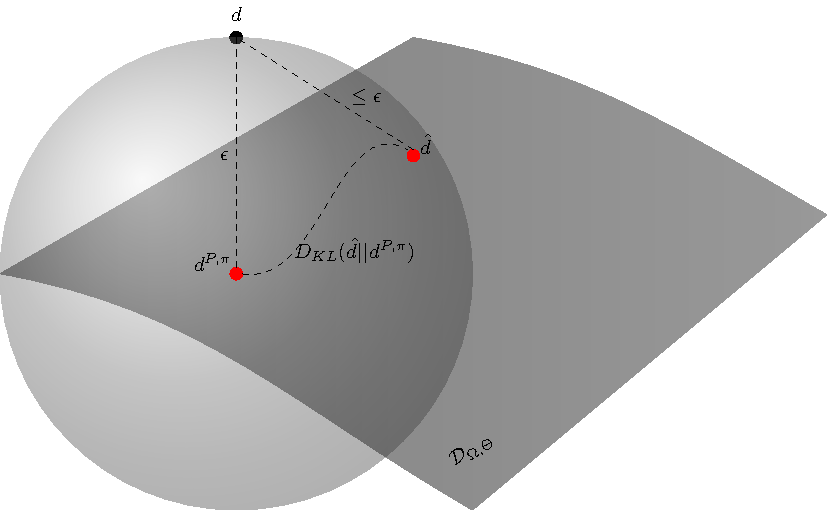
\includegraphics{pictures/Information_projection}
	\caption{Illustration of REMPS and information projection. The ball centred in $d^{P,\pi}$ with radius $\epsilon$ represents the KL constraint over the space of distributions. The surface $\mathcal{D}_{\Omega , \Theta}$ represents the space of available distributions. Distances are not euclidean since measured with the KL divergence.}
\end{figure}

\subsubsection{Projection of the stationary distribution}
In principle, as REMPS works on the stationary distribution, we should project it directly, \ie finding the parameters that induce the most similar stationary distribution. The projection problem is:
\begin{align*}
	& \widehat{\mathbr{\theta}}, \widehat{\mathbr{\omega}} = \argmin_{\mathbr{\theta} \in \Theta, \mathbr{\omega} \in \Omega} D_{KL} \left(d(s,a,s') \| d^{\mathbr{\omega}, \mathbr{\theta}}(s,a,s')\right)  \\
    & s.t. \; d^{\mathbr{\omega}, \mathbr{\theta}}(s) =\int_{\mathcal{S}} \int_{\mathcal{A}}d^{\mathbr{\omega}, \mathbr{\theta}}(s') \pi_{\mathbr{\theta}}(a|s') P_{\mathbr{\omega}}(s'|s,a) \mathrm{d}a \mathrm{d}s'.
\end{align*}
However this problem is impractical as the constraint is difficult to enforce in continuous state-spaces even if replaced with the matching of the expectations of some features. Differently, in finite state-action spaces it is possible to enforce its sample based version by introducing a variable for each $d^{\mathbr{\omega}, \mathbr{\theta}}(s)$.
\subsubsection{Projection of the state kernel $P^{\pi}$}
The projection of the state kernel $P^{\pi}$ is a relaxed version with respect to the stationary distribution projection.
We minimize the expected KL--divergence between $P^{\pi}$ of the distribution $d$ recovered by REMPS and $P_{\mathbr{\omega}}^{\pi_{\mathbr{\theta}}}$, that is the state kernel distribution defined by our parametric space:
\begin{align*}
	\widehat{\mathbr{\theta}}, \widehat{\mathbr{\omega}} & = \argmin_{\mathbr{\theta} \in \Theta, \mathbr{\omega} \in \Omega} \int_{\mathcal{S}} d(s) D_{KL} (P^{\pi}(\cdot|s) \| P_{\mathbr{\omega}}^{\pi_{\mathbr{\theta}}}(\cdot|s)) \mathrm{d}s \\
    & = \argmax_{\mathbr{\theta} \in \Theta, \mathbr{\omega} \in \Omega} \int_{\mathcal{S}} d(s) \int_{\mathcal{S}} P^{\pi}(s'|s) \log P_{\mathbr{\omega}}^{\pi_{\mathbr{\theta}}}(s'|s) \mathrm{d}s' \mathrm{d}s \\
    & = \argmax_{\mathbr{\theta} \in \Theta, \mathbr{\omega} \in \Omega} \int_{\mathcal{S}} d(s) \int_{\mathcal{S}} \int_{\mathcal{A}} \pi'(a|s)P'(s'|s, a) \log P_{\mathbr{\omega}}^{\pi_{\mathbr{\theta}}}(s'|s) \mathrm{d}s' \mathrm{d}s \\
    & = \argmax_{\mathbr{\theta} \in \Theta, \mathbr{\omega} \in \Omega} \int_{\mathcal{S}}\int_{\mathcal{A}}\int_{\mathcal{S}} d(s,a,s') \log \int_{\mathcal{A}} P_{\mathbr{\omega}}(s'|s,a') \pi_{\mathbr{\theta}}(a'|s) \mathrm{d}a' \mathrm{d}s \mathrm{d}a \mathrm{d}s'
\end{align*}
The sample-based version requires to compute the state kernel from samples, this can be done for the case of finite actions (and possibly continuous state-space):
\begin{align*}
	\widehat{\mathbr{\theta}}, \widehat{\mathbr{\omega}} & = \argmax_{\mathbr{\theta} \in \Theta, \mathbr{\omega} \in \Omega} \sum_{(s,a,s') \in \mathcal{D}} \frac{d(s,a,s')}{d^{P,\pi}(s,a,s')} \log \sum_{a' \in \mathcal{A}} P_{\mathbr{\omega}}(s'|s,a') \pi_{\mathbr{\theta}}(a'|s) \\
& = \argmax_{\mathbr{\theta} \in \Theta, \mathbr{\omega} \in \Omega} \sum_{(s,a,s') \in \mathcal{D}} \exp\left(\frac{R
(s,a,s')}{\eta} \right)  \log \sum_{a' \in \mathcal{A}} P_{\mathbr{\omega}}(s'|s,a') \pi_{\mathbr{\theta}}(a'|s) ,
\end{align*}
where $\mathcal{D}$ is a dataset collected with the distribution $d^{P,\pi}$ and we use importance sampling in order to recover the expected value under the distribution $d$ from samples coming from the sampling distribution $d^{P,\pi}$ and we rewrite the ratio $d/d^{P,\pi}$ as:
$$
 \frac{d(s,a,s')}{d^{P,\pi}(s,a,s')} \propto \exp\left(\frac{R
(s,a,s')}{\eta}\right) \; ,
$$
neglecting a constant.
\subsubsection{Projection of policy and model independently}
\label{sec:disjproj}
In this simpler version of the projection problem we minimize the expected KL--divergence between the distributions $\pi'$ and $P'$ and their corresponding parametric distributions $\pi_{\mathbr{\theta}}$ and $P_{\mathbr{\omega}}$.
\begin{align}
	\widehat{\mathbr{\theta}} & = \argmin_{\mathbr{\theta} \in \Theta} \int_{\mathcal{S}} d(s) D_{KL} (\pi'(\cdot|s) \| \pi_{\mathbr{\theta}} (\cdot|s)) \mathrm{d}s = \\
    & = \argmin_{\mathbr{\theta} \in \Theta} \int_{\mathcal{S}} d(s) \int_{\mathcal{A}} \pi'(a|s) \log \frac{\pi(a|s)}{\pi_{\mathbr{\theta}} (a|s)} \mathrm{d}a \mathrm{d}s = \\
    & = \argmin_{\mathbr{\theta} \in \Theta} \int_{\mathcal{S}} \int_{\mathcal{A}}  \int_{\mathcal{S}}  d(s,a,s') \log \frac{\pi'(a|s)}{\pi_{\mathbr{\theta}} (a|s)} \mathrm{d}s \mathrm{d}a \mathrm{d}s' = \\
    & = \argmax_{\mathbr{\theta} \in \Theta} \int_{\mathcal{S}} \int_{\mathcal{A}}  \int_{\mathcal{S}} d(s,a,s') \log \pi_{\mathbr{\theta}} (a|s) \mathrm{d}s \mathrm{d}a \mathrm{d}s',
\end{align}
that can be estimated from samples:
\begin{align}
	\widehat{\mathbr{\theta}} & = \argmin_{\mathbr{\theta} \in \Theta} \sum_{(s,a,s') \in \mathcal{D}} \exp\left(\frac{R(s,a,s')}{\eta} \right) \log \pi_{\mathbr{\theta}} (a|s),
\end{align}
where $\mathcal{D}$ is a dataset collected with $d^{P,\pi}$.
Symmetrically, for the transition model:
\begin{align*}
	\widehat{\mathbr{\omega}} & = \argmin_{\mathbr{\omega} \in \Omega} \int_{\mathcal{S}} \int_{\mathcal{A}} d(s,a) D_{KL} (P'(\cdot|s,a), P_{\mathbr{\omega}} (\cdot|s,a)) \mathrm{d}s \mathrm{d}a= \\
    & = \argmax_{\mathbr{\omega} \in \Omega} \int_{\mathcal{S}} \int_{\mathcal{A}}  \int_{\mathcal{S}} d(s,a,s') \log P_{\mathbr{\omega}} (s'|s,a) \mathrm{d}s \mathrm{d}a \mathrm{d}s',
\end{align*}
and the sample based optimization works as for the policy. This optimization problem can be easily solved in a sample-based form for both finite and continuous state and action spaces.

%\begin{algorithm}[tb]
%  \caption{Relative Entropy Model Policy Search
%    \label{alg:remps}}
%  \begin{algorithmic}[1]
%  \Require{$\epsilon$: KL constraint, $\tilde{P}$: model approximation.}
%  \State Initialize $\pi^{(0)}, P^{(0)}$ randomly
%  \For{t = 0,1,... until convergence}
%  \State Collect samples from $\pi^{(t)}, P^{(t)}$
%  \State Obtain $\eta^*$, the minimizer of the estimated dual problem: 
%  \begin{align*} 
%  \eta^* &= \min_{\eta \geq 0} \widetilde{g}(\epsilon, \eta) \\
%  & = \min_{\eta \geq 0} \eta \log \left[ \frac{1}{N}\sum_{(s,a,s') \sim d^{P,\pi}} \exp \left( \epsilon + \frac{R(s,a,s')}{\eta} \right) \right].	
% \end{align*}
%%  \State Calculate the optimal distribution $d'$:
%%  $$
%%  d'(s,a,s') = \frac{d^{P,\pi}(s,a,s') \exp \left(\frac{R(s,a,s')}{\eta^*} \right)}{\sas d^{P,\pi}(s,a,s') \exp \left( \frac{R(s,a,s')}{\eta^*} \right) \mathrm{d}s \mathrm{d}a \mathrm{d}s'}
%%  $$
%  \State Project the optimal distribution $d'$ onto $\mathcal{D}_{\Omega, \Theta}$ according to the projection strategy. %\newline \hspace*{1.25em} 
%\begin{description}
%  	\item[a.]   Projection of the stationary distribution: \begin{align*}
%	& \widehat{\mathbr{\theta}}, \widehat{\mathbr{\omega}} = \argmin_{\mathbr{\theta} \in \Theta, \mathbr{\omega} \in \Omega} D_{KL} (d(s,a,s') \| d^{\mathbr{\omega}, \mathbr{\theta}}(s,a,s'))  \\
%    & s.t. \; d^{\mathbr{\omega}, \mathbr{\theta}}(s) =\int_{\mathcal{S}} \int_{\mathcal{A}}d^{\mathbr{\omega}, \mathbr{\theta}}(s') \pi_{\mathbr{\theta}}(a|s') \widetilde{P}_{\mathbr{\omega}}(s'|s,a) \mathrm{d}s' \mathrm{d}a.
%\end{align*}
%  	\item[b.]  Projection of the state kernel: $$
%  \widehat{\mathbr{\theta}}, \widehat{\mathbr{\omega}} = \argmax_{\mathbr{\theta} \in \Theta, \mathbr{\omega} \in \Omega} \sum_{(s,a,s') \sim d^{P,\pi}} \exp\left(\frac{R(s,a,s')}{\eta^*} \right) \log \sum_{a' \in \mathcal{A}} \widetilde{P}_{\mathbr{\omega}}(s'|s,a') \pi_{\mathbr{\theta}}(a'|s) .
%  $$
%  \item[c.] Projection of policy and model indendently 
%\begin{align}
%	\widehat{\mathbr{\theta}} & = \argmin_{\mathbr{\theta} \in \Theta} \sum_{(s,a,s') \sim d^{P,\pi}} \exp\left(\frac{R(s,a,s')}{\eta} \right) \log \pi_{\mathbr{\theta}} (a|s), \\
%	\widehat{\mathbr{\omega}} & = \argmin_{\mathbr{\omega} \in \Omega} \sum_{(s,a,s') \sim d^{P,\pi}} \exp\left(\frac{R(s,a,s')}{\eta} \right) \log \widetilde{P}_{\mathbr{\omega}} (s' \mid s, a) .
%\end{align} 
%\end{description}
%  \State Update policy: $\mathbr{\theta}^{(t+1)} \leftarrow \widehat{\mathbr{\theta}}$ 
%  \State Update model: $\mathbr{\omega}^{(t+1)} \leftarrow \widehat{\mathbr{\omega}}$
%  \EndFor \\
%  \Return{Policy-Model Pair ($P^{(t)},\pi^{(t)}$)
%  } 	
%  \end{algorithmic}
%\end{algorithm}


\begin{algorithm}[tb]
  \caption{Relative Entropy Model Policy Search
    \label{alg:remps}}
  \begin{algorithmic}[1]
  \Require{$\epsilon$: KL constraint, $P$: model.}
  \State Initialize $\pi_{\bm{\theta}_0}, P_{\bm{\omega}_0}$ randomly
  \For{t = 0,1,... until convergence}
  \State Collect samples from $\pi_{\bm{\theta}_t}, P_{\bm{\omega}_t}$
  \State Obtain $\eta^*$, the minimizer of the dual problem: 
 \begin{align}
	\eta^* = &\min_{\eta \in [0,+\infty)} g(\eta) \\
	&= \min_{\eta \in [0,+\infty)} \eta \log \left( \sas d^{P,\pi}(s,a,s') \exp \left(\epsilon + \frac{R(s,a,s')}{\eta} \right)\mathrm{d}s \mathrm{d}a \mathrm{d}s' \right).
\end{align}
%  \State Calculate the optimal distribution $d'$:
%  $$
%  d'(s,a,s') = \frac{d^{P,\pi}(s,a,s') \exp \left(\frac{R(s,a,s')}{\eta^*} \right)}{\sas d^{P,\pi}(s,a,s') \exp \left( \frac{R(s,a,s')}{\eta^*} \right) \mathrm{d}s \mathrm{d}a \mathrm{d}s'}
%  $$
  \State Project the optimal distribution $d$ onto $\mathcal{D}_{\Omega, \Theta}$ according to the projection strategy. %\newline \hspace*{1.25em} 
\begin{description}
  	\item[a.]   Projection of the stationary distribution: \begin{align*}
	& \widehat{\mathbr{\theta}}, \widehat{\mathbr{\omega}} = \argmin_{\mathbr{\theta} \in \Theta, \mathbr{\omega} \in \Omega} D_{KL} (d(s,a,s') \| d^{\mathbr{\omega}, \mathbr{\theta}}(s,a,s'))  \\
    & s.t. \; d^{\mathbr{\omega}, \mathbr{\theta}}(s) =\int_{\mathcal{S}} \int_{\mathcal{A}}d^{\mathbr{\omega}, \mathbr{\theta}}(s') \pi_{\mathbr{\theta}}(a|s') P_{\mathbr{\omega}}(s'|s,a) \mathrm{d}s' \mathrm{d}a.
\end{align*}
  	\item[b.]  Projection of the state kernel: $$
  \widehat{\mathbr{\theta}}, \widehat{\mathbr{\omega}} = \argmax_{\mathbr{\theta} \in \Theta, \mathbr{\omega} \in \Omega} \int_{\mathcal{S}}\int_{\mathcal{A}}\int_{\mathcal{S}} d(s,a,s') \log \int_{\mathcal{A}} P_{\mathbr{\omega}}(s'|s,a') \pi_{\mathbr{\theta}}(a'|s) \mathrm{d}a' \mathrm{d}s \mathrm{d}a \mathrm{d}s' .
  $$
  \item[c.] Projection of policy and model independently: 
\begin{align}
	\widehat{\mathbr{\theta}} & = \argmax_{\mathbr{\theta} \in \Theta} \int_{\mathcal{S}} \int_{\mathcal{A}}  \int_{\mathcal{S}} d(s,a,s') \log \pi_{\mathbr{\theta}} (a|s) \mathrm{d}s \mathrm{d}a \mathrm{d}s' \\
	\widehat{\mathbr{\omega}} & = \argmax_{\mathbr{\omega} \in \Omega} \int_{\mathcal{S}} \int_{\mathcal{A}}  \int_{\mathcal{S}} d(s,a,s') \log P_{\mathbr{\omega}} (s'|s,a) \mathrm{d}s \mathrm{d}a \mathrm{d}s'.
\end{align} 
\end{description}
  \State Update policy: $\mathbr{\theta}_{t+1} \leftarrow \widehat{\mathbr{\theta}}$ 
  \State Update model: $\mathbr{\omega}_{t+1} \leftarrow \widehat{\mathbr{\omega}}$
  \EndFor \\
  \Return{Policy-Model Pair $\left( \pi_{\bm{\theta}_t}, P_{\bm{\omega}_t} \right)$
  } 	
  \end{algorithmic}
\end{algorithm}


\subsection{Model Approximation}
In the previous sections we presented REMPS in the case of known environment. However, the perfect knowledge of the environment is difficult, or even impossible, in practice. Even in cases where an environment model is available it might be too approximate or hardy usable being very complex and computationally expansive. \newline In REMPS it is possible to use any model approximation method, the only requirement is that it must be possible to learn the mapping $(s, a , \boldsymbol{\omega}) \rightarrow s'$, from state, action and environment configuration to a distribution over the next states. Notice that in REMPS the environment model is used only the projection phase, while the optimization phase is model-free. \newline
In order to learn an environment approximation we use a maximum likelihood (ML) approach. We collect a dataset composed by tuples $(s, a,\boldsymbol{\omega}, s')$ and given a parametric model defining a distribution over the state space we find the parameters by maximizing the log-likelihood of the seen transitions. The parametric model can be a Gaussian Process, a Neural Network or some other function approximator model. We denote the model approximation with $\widetilde{P}$. \newline
\subsection{Discussion}
In this section we discuss the main benefits and limitations of REMPS.
Being an information theoretic approach, REMPS, has the main goal of maximizing the performance while staying close to the observed data. This translates into the KL constraint between the sampling distribution $d^{P,\pi}$ and the optimized distribution $d$. REMPS considers jointly the effect of the two CMDP components and finds a distribution, in the space of all possible distributions, maximizing the average reward while satisfying the KL constraint using a primal-dual formulation. However, due to a possible limitation in the representation power of the model and the policy this distribution might be unfeasible. Notice that a lack in representation power of the policy can be easily addressed (e.g. using more parameters), while a limited representation power in the model has to be expected since the number of parameters and their influence is fixed given a task. REMPS solves this problem by performing a KL--projection, that is finding the model-policy pair minimizing the KL distance between their joint distribution $\hat{d}$ and $d$. \newline
Having access to infinite samples we are sure that $d$ is close the sampling distribution, that is $D_{KL}(d \| d^{P,\pi}) \le \epsilon$. This constraint might be, in practice, not satisfied due to wrong estimations. 
We also highlight the fact that performing the Moment Projection we can actually find a suboptimal distribution. By a simple inspection we can easily prove that $D_{KL}(d \| \widehat{d}) \le \epsilon$. However, being the KL--divergence not symmetric, we have no insight on $D_{KL}(\widehat{d} \| d^{P,\pi})$ that is a more relevant quantity. \newline
In practice we can add a regularization in the projection phase penalizing some type of distance between the new model-policy parameters and the sampling parameters, even if this is not theoretically justified. \newline
The REMPS pseudocode is reported in \cref{alg:remps}.

\clearpage
%%%%%%%%%%%%%%%%%%%% THEORY %%%%%%%%%%%%%%%%%%%%%%%%%%%
%\section{Theoretical Analysis}\label{sec:remps-theory}
%In this section we derive some theoretical guarantees for REMPS when it is executed starting from a finite number of samples $N$. In the following table are compared the exact and approximate version of REMPS. We denote as $\mathcal{X}=\mathcal{S} \times \mathcal{A} \times \mathcal{S}$ the state-action-next-state space, with $x=(s,a,s') \in \mathcal{X}$. For ease of notation we use $w(x)=\widetilde{p}(x)/q(x)$.
%This analysis is based on \citep{cortes2010}.
%
%\begin{small}
%\begin{tabular}{|m{5.3cm}|m{5.3cm}|}
%\hline
%  	\begin{center}	\remps	\end{center}
%    {\begin{align*}
%	& \max_p J_p = \int_\mathcal{X} p(x)R(x) dx \\
%	s.t. \quad & D_{KL}(p||q) = \int_\mathcal{X} p(x) \log \frac{p(x)}{q(x)} dx \leq \epsilon \\
%	& \int_\mathcal{X} p(x) dx = 1
%	\end{align*}} & 
%	\begin{center}	\rempstilde	\end{center}
%	{\begin{align*}
%		& \max_{\widetilde{p}} J_{\widetilde{p}/q}^N = \frac{1}{N} \sum_i w(x_i)R(x_i) dx \\
%		s.t. \quad &  \widetilde{D}_{KL, \widetilde{p}/q}(\widetilde{p}||q) = \sum_i w(x_i) \log w(x_i) dx \leq \epsilon \\
%		& \frac{1}{N} \sum_i w(x_i) = 1
%	\end{align*}} \\
%	\hline
%	\begin{center} $\mathrm{DUAL}$ \end{center}
%	{\begin{equation*}
%		\min_{\eta \geq 0} \frac{1}{\eta} \log \int_\mathcal{X} q(x) \exp(\eta R(x) + \epsilon) dx
%	\end{equation*}}
%	&
%	\begin{center} $\mathrm{\widetilde{DUAL}}$ \end{center}
%	{\begin{equation*}
%		\min_{\widetilde{\eta} \geq 0} \frac{1}{\widetilde{\eta}} \log \frac{1}{N}\sum_i \exp (\widetilde{\eta} R(x) + \epsilon)
%	\end{equation*}
%	} \\
%	\hline
%	\begin{center} $\mathrm{PROJ}$ \end{center}
%	{\begin{equation*}
%		\min_{p' \in \mathcal{P}} D_{KL}(p || p') = \int_\mathcal{X} p(x) \log \frac{p(x)}{p'(x)} dx
%	\end{equation*}}
%	& \begin{center} $\mathrm{\widetilde{PROJ}}$ \end{center}
%	{
%	\begin{equation*}
%		\min_{\widetilde{p}' \in \mathcal{P}} D_{KL, \widetilde{p}/q}^N(\widetilde{p} || \widetilde{p}') = \frac{1}{N} \sum_i w(x_i) \log \frac{\widetilde{p}(x_i)}{\widetilde{p}'(x_i)}
%	\end{equation*}} \\
%	\hline
%\end{tabular}
%\end{small}
%Thus we have defined an exact version and an approximate version of the REMPS problem. We have that the approximated version approaches to the exact one when an infinite number of samples is available. In this section we want to formalize this idea.
%The approximated version deals with an off-policy estimation of the relevant quantities, performed by means of an importance weighting like technique.
%The solution of the exact version of REMPS and the approximated version are:
%\begin{align*}
%	& p(x)=\frac{q(x)\exp(\eta R(X))}{\int_\mathcal{X}q(x)\exp(\eta R(x)dx}
%	& \widetilde{p}(x)=\frac{q(x)\exp(\widetilde{\eta} R(x)}{\frac{1}{N}\sum_i \exp(\widetilde{\eta} R(x))}  \; .
%\end{align*} 
%We denote with $\hat{w}(x)$ the ratio importance weight, and with $\widetilde{w}(x)$ the self normalized importance weight:
%\begin{align*}
%	& \hat{w}(x)=\frac{\exp(\eta R(X))}{\int_\mathcal{X}q(x)\exp(\eta R(x))dx}
%	& \widetilde{w}(x) = \frac{\exp(\widetilde{\eta} R(x))}{\sum_i \exp(\widetilde{\eta} R(x))} = \frac{w(x)}{N}  \; .
%\end{align*} 
%We can notice that the quantity being maximized in $\mathrm{\widetilde{REMPS}}$ it is actually a self-normalized importance weighting estimate, opposed to the ratio importance weighting estimate $\hat{J}$ not appearing in the optimization problems:
%\begin{align*}
%	& \hat{J} = \frac{1}{N}\sum_i \hat{w}(x_i)R(x_i)
%	& \widetilde{J} = \sum_i \widetilde{w}(x_i) R(x_i) \; .
%\end{align*}
%The ratio estimate is unbiased while the self-normalized estimate is biased but consistent.
%
%\subsection{Preliminaries}
%In this section, we provide some results that will be used in the following sections.
%\paragraph{Preliminary results} Our analysis use the notion of Rényi divergence, an information theoretical measure of the difference between two distributions. It is very important in the study of importance weighting. We denote the Rényi divergence with $D_\alpha (p || q)$:
%\begin{equation}	
%D_\alpha (p || q) = \frac{1}{\alpha - 1}log_2 \sum_x p(x) \left( \frac{p(x)}{q(x)} \right)^{\alpha -1} \, ,
%\end{equation} 
%for $\alpha \geq 0$.
%The Rènyi divergence is a non negative quantity for any $\alpha>0$ and it coincides with the Relative entropy with $\alpha=1$. It is important also the exponential base 2 of the Rènyi, denoted as $d_\alpha (p || q)$:
%\begin{equation}
%	d_\alpha (p || q)= \left[ \sum_x p(x) \frac{p(x)}{q(x)}^{\alpha-1} \right]^{\frac{1}{\alpha - 1}}
%\end{equation}
%The exponentiated 2-Rényi divergence has the following form:
%\begin{equation}
%	d_2 (p || q)= \left[ \sum_x p(x) \frac{p(x)}{q(x)} \right]
%\end{equation}
%The following identities are standard results from the analysis of importance weights:
%\begin{align}
%	&\mathbb{E} \hat{w}=1 \\ &\mathbb{E}\left[ \hat{w}^2 \right]=d_2(p || q) \\  &\sigma^2( \hat{w}) = d_2 (p || q) - 1
%\end{align}
%Let us demonstrate the second identity:
%\begin{align}
%	\mathbb{E} \left[ \hat{w}^2 \right] &= \sum \hat{w}(x)^2 q(x) \\
%										&= \sum \left( \frac{p(x)}{q(x)} \right)^2 q(x) \\
%										&= \sum \frac{p(x)^2}{q(x)}
%\end{align}
%
%\paragraph{Learning bound for self-normalized importance weighting} We start observing that in our peculiar case the choice of $p$ in the hypothesis space $\mathcal{P}$ has an effect on the weights $p(x)$ rather than on the loss function of a single sample, which is fixed being the reward function $R(x)$.
%We consider the more general case in which both the loss function and the weights can vary. We denote as $d_{\mathcal{P}, \mathcal{F}}=Pdim(\{\widetilde{w}(x)f(x) : \widetilde{w}(x) = p(x)/q(x), p \in \mathcal{P}, f \in \mathcal{F}\})$,  $d_{\mathcal{P}}=Pdim(\{\widetilde{w}(x) : \widetilde{w}(x) = p(x)/q(x), p \in \mathcal{P}\})$ the pseudo dimension of the class of weights, $d = \max\{d_{\mathcal{P}, \mathcal{F}},d_{\mathcal{P}}\}$. We assume that $d < \infty$.
%We derive the following bounds for self-normalized importance weights, which combines Theorem3 of [cortes2010] and the result of the relationship between ratio importance weights and self normalized importance weights:
%
%\begin{theorem}
%	Let $d$ as defined before, $d_2(p || q)$ the exponentiated Rényi 2 divergence and $\hat{d}_2(p || q) = \frac{1}{N} \sum_i \hat{w}(x_i)$ its estimate. Define $M=\sup_{p \in \mathcal{P}}\max\{\sqrt{d_2(p||q)},\sqrt{\hat{d}_2(p||q)}$, the suprema over the distribution family of the maximum between the true $d_2$ and its estimated version. Assume that $d_2(p||q) < \infty$, and for all $f \in \mathcal{F}$, we have that $||f||_\infty < \infty$. Then for any $\delta$ with probability at least $1-\delta$, the following bound holds:
%	\begin{equation}
%		\left| \underset{x \sim p}{\mathbb{E}} \left[ f(x) \right] - \sum_i \widetilde{w}(x_i)f(x_i) \right| \leq 2 ||f||_\infty \min \left\{ 1, \frac{M}{8} \left( \frac{d\log \frac{2eN}{d} + \log \frac{16}{\delta}}{N} \right)^{3/8} \right\}
%	\end{equation}
%	\label{thr:learning-theory}
%\end{theorem}
%
%This bound relates the difference between the expected value of a quantity and its empirical expectation using a self-normalized importance weighting technique.
%
%\begin{proof}
%	Being $|f(x)| \leq ||f||_\infty$ the bound cannot be larger than $2||f||_\infty$. The idea of the proof is to use the ratio estimator and bound in probability its difference with the self-normalized estimator and its variance.
%	\begin{equation}
%		\left| \underset{x \sim p}{\mathbb{E}} \left[ f(x) \right] - \sum_i \widetilde{w}(x_i)f(x_i) \right| \leq  \left| \underset{x \sim p}{\mathbb{E}} \left[ f(x) \right] - \frac{1}{N}\sum_i \hat{w}(x_i)f(x_i) \right| + \left| \frac{1}{N}\sum_i \hat{w}(x_i)f(x_i) -  \sum_i \widetilde{w}(x_i)f(x_i) \right| \, .
%	\end{equation}
%	The first term is the difference between the expected value of a function and its empirical expectation using the ratio importance weighting. This can be bounded using theorem 3 of cortes:
%	\begin{equation}
%		\left| \underset{x \sim p}{\mathbb{E}} \left[ f(x) \right] - \frac{1}{N}\sum_i \hat{w}(x_i)f(x_i) \right| \leq 2^{5/4} ||f||_\infty M \left( \frac{d_{\mathcal{P},\mathcal{F}} \log \frac{2eN}{d_{\mathcal{P},\mathcal{F}}} + \log \frac{8}{\delta}}{N} \right)^{3/8} \, .
%	\end{equation}
%	Consider now the second term, we can use the following inequality and apply again the same theorem as before:
%	\begin{align}
%		\left| \frac{1}{N}\sum_i \hat{w}(x_i)f(x_i) -  \sum_i \widetilde{w}(x_i)f(x_i) \right| &= \left| \sum_i\widetilde{w}(x_i)f(x_i) \left( 1 - \frac{\sum_i \hat{w}(x_i)}{N} \right) \right| \\
%		& \leq ||f||_\infty \left| 1 - \frac{\sum_i \hat{w}(x_i)}{N} \right| \
%	\end{align}
%	We have that, as demonstrated before, $1$ is the mean of the ratio estimator. So this is the discrepancy between the average weight and its mean. We can apply theorem 3 both sides, and w.p. at least $1-\delta$:
%	\begin{equation}
%		\left| \frac{1}{N}\sum_i \hat{w}(x_i)f(x_i) -  \sum_i \widetilde{w}(x_i)f(x_i) \right| \leq 2^{5/4} ||f||_\infty M \left( \frac{d_{\mathcal{P}} \log \frac{2eN}{d_{\mathcal{P}}} + \log \frac{8}{\delta}}{N} \right)^{3/8}
%	\end{equation}
%	We can now use a union bound obtaining, w.p. $1-2\delta$:
%	\begin{equation}
%		\left| \underset{x \sim p}{\mathbb{E}} \left[ f(x) \right] - \sum_i \widetilde{w}(x_i)f(x_i) \right| \leq 2 ||f||_\infty \min \left\{ 1, \frac{M}{8} \left( \frac{d\log \frac{2eN}{d} + \log \frac{8}{\delta}}{N} \right)^{3/8} \right\}
%	\end{equation}
%	Replacing $\delta$ with $\delta/2$ we obtain the result.
%\end{proof}
%
%\paragraph{Sensitivity Analysis on the KL divergence constraint} Since the KL constraint of REMPS is estimated from samples too, we need to understand how the performance of the solution changes when using a different $\epsilon$. \newline
%
%$\epsilon' < \epsilon$ In this case the constraint is more restrictive, thus we expect $J_p' < J_p$ where $p'$ is the optimal solution (with infinite samples) having $\epsilon'$ as KL constraint and $p$ the solution with $\epsilon$. 
%Consider a new \textit{class distributions} $p_\alpha = \alpha p + (1 - \alpha)q$, a convex combination of $p$ and $q$. Ideally, we could increase $\alpha$ until we satisfy the constraint $\epsilon'$ getting the best representation of $p$ fullfilling the constraint, yielding a certain $\alpha'$. We are able to provide a lower bound on $\alpha'$ depending on the two coefficients $\epsilon$ and $\epsilon'$.
%
%\begin{lemma}
%	Let $p_\alpha = \alpha p + (1 - \alpha)q$, the value of $\alpha'$ s.t. $D_{KL}(p_\alpha' || q) = \epsilon'$ can be lower bounded as:
%	\begin{equation}
%		\alpha \geq \frac{\epsilon'}{\epsilon} 
%	\end{equation}
%\end{lemma}
%\begin{proof}
%	We use the convexity of the KL divergence: $D_{KL}(\alpha \mu_1 + (1-\alpha) \mu_2 || \alpha \nu_1 + (1-\alpha) \nu_2) \leq \alpha D_{KL}(\mu_1 || \nu_1) + (1-\alpha) D_{KL}(\mu_2 || \nu_2)$. Take $\mu_1=p, \mu_2 = \nu_1 = \nu_2 = q$:
%	\begin{align}
%		\epsilon' &= D_{KL}(p_\alpha || q) \leq \alpha D_{KL}(p || q) \\
%				  & \leq \alpha \epsilon
%	\end{align}
%	By inverting the relation the result follows.
%\end{proof}
%Now we are ready to state the main result. 
%\begin{prop}
%Let $p$ and $p'$ defined before. The following bound holds:
%\begin{equation}
%	J_p - J_p' \leq R_{max} \left( 1 - \frac{\epsilon'}{\epsilon} \right) || p - q ||_1
%\end{equation}	
%\end{prop}
%
%\begin{proof}
%	We observe that being $p'$ the optimal solution with constraint $\epsilon'$ and since $p_{\alpha'}$ fullfills the constraint we surely have $J_{p'} \geq J_{p_\alpha'}$.
%	\begin{align}
%		J_p - J_{p'} &\leq J_p - J_{p_\alpha'} \\
%					 &\leq R_{max} ||p - p_{\alpha'}||_1 \\
%					 & \leq R_{max} ||(1-\alpha')(p - q)||_1 \\
%					 & \leq  R_{max} (1-\alpha') ||p-q||_1
%	\end{align}
%	By using the previous lower bound on $\alpha$:
%	\begin{equation}
%		1 - \alpha' \leq 1 - \frac{\epsilon'}{\epsilon} \, .
%	\end{equation}
%	Combining the two previous inequality we obtain the result.
%\end{proof} 
%
%$\epsilon' > \epsilon$ We have a more relaxed constraint. We do not need to bound this quantity.
%
%\subsection{Finite-sample analysis}
%Before going into the details of the analysis let us focus on the main hypothesis space we will consider and the main assumptions we are going to make. 
%\begin{itemize}
%	\item $\mathcal{P}_q = \{p(x) \propto q(x) \exp (\eta R(x) : \eta \in [0,+\infty] \}$. This is the space of distributions considered int he optimization of REMPS and the dual.
%	\item $\mathcal{P}$ as defined before is a subspace of distributions.
%\end{itemize}
%\begin{ass}
%	We assume the following:
%	\begin{itemize}
%		\item (Finite dimension) We assume $d=\max\{Pdim(\{p(x)/q(x), p \in \mathcal{P}_q\}), Pdim(\{(p(x)/q(x))R(x), p \in \mathcal{P}_q\}\} < \infty$. Moreovere $\tilde{d} = Pdim(\mathcal{P}) < \infty$.
%		\item (Finite Rényi divergence) There exists $\beta>2$ s.t. $d_\beta(p||q) < \infty$ for all $p \in \mathcal{P}_q$.
%		\item (Uniformly bounded reward) $sup_{x \in \mathcal{X}} |R(x)| \leq R_{max} < \infty$.
%	\end{itemize}
%	\label{ass:remps}
%\end{ass}
%
%\paragraph{Goal} Our main goal is to provide a bound to the quantity $J_p - J_{\tilde{p}'}$, i.e. the difference on the performance between the exact solution and the projection of solution using a finite number of samples. In order to this we decompose the problem into the REMPS problem and the projection problem:
%\begin{equation}
%	J_p - J_{\tilde{p}'} = \underbrace{J_p - J_{\widetilde{p}}}_{\mathrm{REMPS/dual}} + \underbrace{J_{\widetilde{p}}- J_{\widetilde{p}'}}_{\mathrm{proj}}.
%\end{equation}
%
%\paragraph{First term:} $J_p - J_{\widetilde{p}}$. This is the difference in (true) performance between the optimal solution having infinite number of samples and the performance of the empirical risk minimizer (ERm). A typical approach from Empirical Risk Minimization (ERM) is to add and subtract the empirical risk of the ERm exploiting the fact that this quantity is larger than (smaller in supervised learning) than the empirical risk of any other hypothesis in the hypothesis space (from the definition of the ERm), in particular $p$. In our framework the hypothesis space changes since the KL constraint is estimated from samples and it can impose more relaxed or tight conditions. We introduce a new distribution $\bar{p}$ which is the optimal solution of the exact REMPS problem using the sample constraint. For this reason $\bar{p}$ and $\tilde{p}$ are searched in the same hypothesis space and we can apply theory from ERM. 
%We need to define the discrepancy in the constraint for a given hypothesis $p$:
%\begin{equation}
%	\Delta\epsilon(p) = D_{KL}(p||q) - \tilde{D}_{KL, p/q}^N(p||q).
%\end{equation} 
%As a consequence:
%\begin{align}
%	  \tilde{D}_{KL, p/q}^N(p||q) \leq \epsilon \iff D_{KL}(p||q) \leq \epsilon + \Delta\epsilon(p) .
%\end{align}
%Finally we define $\Delta\epsilon = sup_{p \in \mathcal{P}_q} \Delta\epsilon(p)$.In other words $\Delta\epsilon$ is the suprema, over all hypothesis considered of the discrepancy between the exact KL and the estimated one using the self-normalized importance weights.
%We have two cases: \begin{itemize}
%	\item $\Delta\epsilon \leq 0$, the exact constraint is always tighter, thus $J_{\bar{p}} \geq J_p$. 
%	\item $\Delta\epsilon > 0$, there exists at least one hypothesis in $\mathcal{P}_q$ such that the exact constraint is looser, it might be $J_{\bar{p}} < J_p$. 
%\end{itemize} 
%The following result hold in general:
%\begin{lemma}
%Let $p$ and $\bar{p}$ as defined before:
%\begin{equation}
%	J_p - J_{\bar{p}} \leq \frac{2R_{\max}}{\epsilon} \Delta \epsilon_{+} \, ,
%\end{equation}
%where $\Delta \epsilon_{+} = \max\{0, \Delta\epsilon\}$ .
%\end{lemma}
%\begin{proof}
%If $J_p - J_{\bar{p}} < 0$ the theorem holds. Otherwise it must be $\Delta\epsilon(p) \geq 0$.
%	We define $p_\alpha$ as in the previous proposition:
%	\begin{align}
%		J_p - J_{\bar{p}} & \leq J_p - J_{p_\alpha} \\
%		& \leq R_{\max} \left( 1 - \frac{\epsilon}{\epsilon + \Delta \epsilon(p)} \right) ||p - q||_1 \\
%		& \leq R_{\max} \frac{\Delta\epsilon(p)}{\epsilon + \Delta\epsilon(p)} || p - q||_1 \\
%		& \leq R_{\max} \frac{\Delta \epsilon(p)}{\epsilon}||p - q||_1 \\
%		& \leq R_{\max} \frac{\Delta \epsilon}{\epsilon}||p - q||_1 \\
%		& \leq 2R_{\max} \frac{\Delta \epsilon}{\epsilon} \, ,
%	\end{align}
%	where we used the fact that $||p-q||_1 \leq 2$ ($||p-q||_1$ is total divergence between $p$ and $q$), $\frac{\Delta\epsilon(p)}{\epsilon + \Delta\epsilon(p)} \leq \frac{\Delta\epsilon(p)}{\epsilon}$ being $\Delta\epsilon(p) \geq 0$ and finally $\Delta\epsilon(p) \leq \Delta\epsilon$. Taking the maximum between the two cases we get the result.
%\end{proof}
%
%\paragraph{Bounding $\Delta\epsilon_{+}$} Notice that $\max_{0,\Delta\epsilon} \leq | \Delta\epsilon | = \sup_{p \in \mathcal{P}} | \tilde{D}_{KL, p/q}^N(p||q) - D_{KL}(p||q)|$, which can be used with ERM theory. Assume that $\Delta\epsilon_{+} \leq \epsilon_2$.
%
%We are ready now to give our main result of this theoretical analysis. The following theorem bounds the difference between the performance of the optimal solution and the performance of the solution found with a finite number of samples.
%
%\begin{theorem}[REMPS bound]
%Let $p$ and $\tilde{p}$ be the solution of \remps and \rempstilde problems, the latter using N i.i.d. samples collected from $q$. Let $\epsilon > 0$ be the KL constraint. Then, under Assumptions \ref{ass:remps}, for any $\delta \in (0,1)$, w.p. at least $1-\delta$, it holds that:
%\begin{equation}
%	J_p - J_{\tilde{p}} \leq 4R_{\max} \min \left\{1, \frac{M}{8} \left( \frac{d\log \frac{2eN}{d} + \log \frac{16}{\delta}}{N} \right)^{3/8} \right\} + \frac{2R_{\max}}{\epsilon} \epsilon_2 	\, .
%\end{equation}
%\end{theorem}
%\begin{proof}
%	We use very simple arguments of ERM. Let $\bar{p}$ as defined before, remember that $\tilde{p}$ is the ERm.
%	\begin{align}
%	J_p - J_{\tilde{p}} &\leq J_{\bar{p}} - J_{\tilde{p}} + \frac{2R_{\max}}{\epsilon} \Delta \epsilon_{+} \\
%	& \leq J_{\bar{p}} - J_{\tilde{p}} +\frac{2R_{\max}}{\epsilon} \Delta \epsilon_{+} \pm \widetilde{J}_{\tilde{p}} \\
%	& \leq J_{\bar{p}} - \widetilde{J}_{\tilde{p}} + \widetilde{J}_{\tilde{p}} - J_{\tilde{p}} + \frac{2R_{\max}}{\epsilon} \Delta \epsilon_{+} \\
%	& \leq J_{\bar{p}} - \widetilde{J}_{\bar{p}} + \widetilde{J}_{\tilde{p}} - J_{\tilde{p}} + \frac{2R_{\max}}{\epsilon} \Delta \epsilon_{+} \\
%	& \leq 2\sup_{p \in \mathcal{P}} |J_p - \widetilde{J}_p| + \frac{2R_{\max}}{\epsilon} \Delta \epsilon_{+} \, ,
%	\end{align}
%	where we used the fact that $\widetilde{J}_{\bar{p}} \leq \widetilde{J}_{\tilde{p}}$, being $\tilde{p}$ the ERm over the same hypothesis space. 
%	Now we can apply theorem \ref{thr:learning-theory} in order to bound the first term:
%	\begin{equation}
%		\sup_{p \in \mathcal{P}} |J_p - \widetilde{J}_p| \leq 2 R_{\max} \min \left\{1, \frac{M}{8} \left( \frac{d\log \frac{2eN}{d} + \log \frac{16}{\delta}}{N} \right)^{3/8} \right\}	\end{equation} \, .
%\end{proof}
%
%\paragraph{Second Term: $J_{\tilde{p}} - \tilde{J}_{\tilde{p}'}$} This second term is related to the power of the approximation approximation space considered for the projection. It is useful to recall the property of the KL divergence:
%\begin{equation}
%	D_{KL}(p||q) = H(p||q) - H(p) \, ,
%\end{equation}
%where $H(p||q)$ is the cross-entropy between p and q, $H(p||q) = \int_\mathcal{X} p(x) \log q(x)$, and $H(p)$ is the entropy of $p$. When performing the projection, minimizing the KL divergence, we are actually minimizing the cross-entropy term, since the entropy does not depend on $q$.

\section{Theoretical Analysis}\label{sec:remps-theory}
In this section we derive some theoretical guarantees for the single step of REMPS when it is executed starting from a finite number of samples $N$. This analysis is based on \citep{cortes2010}.
\paragraph{Notation}
Let $d$ be a stationary distribution, we will denote with \newline $\mathcal{D}_d = \left\{d'=\frac{d \exp \left( \frac{1}{\eta}r \right)}{\int d \exp \left( \frac{1}{\eta}r \right)}: \eta \in [0,+\infty) \right\}$. Given a policy hypothesis space $\Pi$ and a transition model hypothesis space $\mathcal{P}$, we will denote with $\mathcal{D}_{\mathcal{P}, \Pi} = \{ d_{P,\pi} : P \in \mathcal{P}, \pi \in \Pi \}$ the set of stationary distributions induced by the policy and model hypothesis spaces.
For the sake of brevity we will denote with $\mathcal{X} = \mathcal{S} \times \mathcal{A} \times \mathcal{S}$ the state-action-next state space and with $x = (s, a, s')$ a state-action-next-state triple. Given a set $\mathcal{X}$, we denote with $\Delta(\mathcal{X})$ the set of probability distributions on $\mathcal{X}$.

\subsection{Problem Formulation}
In this section we revisit the REMPS problem formulation in order to understand better its component to perform a theoretical analysis.
The REMPS problem takes as input a KL-divergence threshold and provides as output a new stationary distribution on the space $\mathcal{D}_{\mathcal{P},\Pi}$.
As we said before, our algorithm is divided in two phases: \textit{optimization} and \textit{projection}.
\paragraph{Optimization} The problem we aim to solve in the optimization phase can be stated as follows. Given a KL-divergence threshold $\epsilon>0$, let $(P,\pi) \in \mathcal{P} \times \Pi$ be the current configuration-policy pair inducing a stationary distribution $d^{P,\pi}$, we seek for a new stationary distribution $d$ that solves the optimization problem $\text{OPT}_{P,\pi}(\epsilon)$:
\begin{align}
	\underset{d \in \Delta{\mathcal{X}}}{\max} J_d &= \underset{x \sim d}{\mathbb{E}} \left[ R(x) \right] \\
	\text{s.t.} & \;\; D_{KL}(d||d^{P,\pi}) = \underset{x \sim d}{\mathbb{E}} \left[ \log \frac{d(x)}{d^{P,\pi}(x)} \right] \leq \epsilon.
\end{align}
The solution of $\text{OPT}_{P,\pi}(\epsilon)$ is:
\begin{equation}
	d(x) = 	\frac{d^{P,\pi}(x) \exp \left( \frac{1}{\eta}R(x) \right)}{\int_{\mathcal{X}}d^{P,\pi}(x) \exp \left( \frac{1}{\eta}R(x) \right) \mathrm{d}x}, x \in \mathcal{X},
\end{equation}
where $\eta$ is the unique solution of the dual problem $\text{DUAL}_{P,\pi}(\epsilon)$:
\begin{equation}
	\min_{\eta \in [0, +\infty)} \eta \log \underset{x \sim d^{P,\pi}}{\mathbb{E}} \exp  \left( \frac{1}{\eta} R(x) + \epsilon \right).
\end{equation}

In practice we have access neither to $d^{P,\pi}$ nor to $d$. Therefore we need to estimate expectations with samples averages from samples collected with the distribution $d^{P,	\pi}$. Notice that we have only access to an empirical estimate of $d^{P,	\pi}$, which is $\widehat{d}^{P,	\pi} = \frac{1}{N} \sum_{i=1}^{N} \delta(x - x_i)$ uniform on the seen $x$s. For this purpose we perform an importance sampling procedure. We define the weights $w(x_i) = \frac{d(x_i)}{\widehat{d}^{P,\pi}(x_i)} = N d(x_i)$. Thus, the approximated problem we need to solve is actually $\widetilde{\text{OPT}}_{P,\pi}(\epsilon)$:
\begin{align}
\max_{d \in \Delta(\{x_i : i \in \{1,2,...,N\} \} )} & \widetilde{J}_d = \frac{1}{N} \sum_{i=1}^N w(x_i) R(x_i) = \sum_{i=1}^N d(x_i) R(x_i) \\
\text{s.t.} & \; \; \widetilde{D}_{KL}(d||d^{P,\pi}) = \frac{1}{N} \sum_{i=1}^N w(x_i) \log w(x_i) = \\ & \qquad \qquad \qquad \; = \sum_{i=1}^N d(x_i) \log d(x_i) + \log N \leq \epsilon .
\end{align}
This problem yields a solution which is defined only over the seen state-action-next state triples:
\begin{equation}
	d(x_i) = \frac{\exp \left( \frac{1}{\widetilde{\eta}} R(x_i) \right)}{\frac{1}{N}\sum_{j=1}^N \left( \frac{1}{\widetilde{\eta}} R(x_j) \right)} , \; \; i \in \{1,2,..., N\},
\end{equation}
where $\widetilde{\eta}$ is the unique solution of the approximated dual problem $\widetilde{\text{DUAL}}_{P,\pi}(\epsilon)$:
\begin{equation}
	\min_{\eta \in [0,+\infty)} \eta \log \frac{1}{N} \sum_{i=1}^N \left( \frac{1}{\widetilde{\eta}} R(x_i) + \epsilon \right) .
\end{equation}
Once solved this problem, the new distribution over the whole space $\mathcal{X}$ is characterized only by the Lagrange multiplier $\widetilde{\eta}$:
\begin{equation}
	\widetilde{d}(x) = \frac{d^{P,\pi}(x) \exp \left( \frac{1}{\widetilde{\eta}} R(x) \right)}{\int_{\mathcal{X}} d^{P,\pi}(x) \exp \left( \frac{1}{\widetilde{\eta}} R(x) \right)} , \; x \in \mathcal{X} .
\end{equation}
We denote the performance of the new stationary distribution $\widetilde{d}$ as with $J_{\widetilde{d}}= \mathbb{E}_{x \sim \widetilde{d}} \left[ R (x) \right]$. As expected we would like find $\widetilde{d}$ maximizing $J_{\widetilde{d}}$ but we actually use an empirical estimate $\widetilde{J}_{\widetilde{d}}$.

\paragraph{Projection} In the \textit{Projection} phase we aim to find the best representation of the stationary distribution we got from the optimization phase given hypothesis space $\mathcal{D}_{\mathcal{P}, \Pi}$. Let $d$ be the solution of $\text{OPT}_{P,\pi}(\epsilon)$, the projection problem $\text{PROJ}_{\mathcal{D}_{P,\Pi}}(d)$ can be stated as the moment-projection of $d$ onto $\mathcal{D}_{\mathcal{P},\Pi}$:
\begin{equation}
	\max_{d' \in \mathcal{D}_{\mathcal{P}, \Pi}} H(d||d') = \underset{x \sim d}{\mathbb{E}} \left[ \log d'(x) \right],
\end{equation}
where we considered the cross-entropy $H(d||d')$ instead of the KL--divergence, since \newline $D_{KL}(d||d')= H(d||d') - H(d)$ and the entropy term $H(d)$ is independent on $d'$. We call $d'$ the solution of this problem, which can be considered the solution of the complete problem $\text{REMPS}_{P,\pi}(\epsilon) = \text{PROJ}_{\mathcal{D}_{\mathcal{P}, \Pi}}(\cdot) \circ \text{OPT}_{P,\pi}(\epsilon)$. Clearly, also in the projection phase we need to consider the Monte Carlo estimates again obtained by the very same samples $\{x_i\}_{i=1}^N$ collected with the sampling distribution $d^{P,\pi}$. Let $\widetilde{d}$ be the solution of $\widetilde{\text{OPT}}_{P,\pi}(\epsilon)$, the approximated projection problem $\widetilde{\text{PROJ}}_{\mathcal{D}_{\mathcal{P},\Pi}}(\widetilde{d})$ becomes:

\begin{equation}
	\max_{d' \in \mathcal{D}_{\mathcal{P}, \Pi}} \widetilde{H}(\widetilde{d}||d') = \frac{1}{N} \sum_{i=1}^N w(x_i) \log d'(x_i) .
\end{equation}
We call $\widetilde{d}'$ the solution of this problem, which can be considered the solution of the complete approximated problem $\widetilde{REMPS}_{P,\pi}(\epsilon) = \widetilde{\text{PROJ}}_{\mathcal{D}_{\mathcal{P},\Pi}}(\cdot) \circ \widetilde{\text{OPT}}_{P,\pi}(\epsilon)$.

\paragraph{Off-distribution estimation}
Given a value of the Lagrange multiplier $\eta$ inducing the distribution $d$, let us define the ratio importance weight $\widehat{w}(x)$ and the self-normalized importance weight $\widetilde{w}(x)$ as:
\begin{align*}
	\widehat{w}(x) &= \frac{d(x)}{d^{P,\pi}(x)} =\\ &= \frac{\exp \left( \frac{1}{\eta} R(x) \right)}{\int_{\mathcal{X}} d^{P,\pi}(x) \exp \left( \frac{1}{\eta} R(x) \right) \mathrm{d}x}, \\
	 \widetilde{w}(x) &= \frac{\widehat{w}(x)}{\sum_{i=1}^N \widehat{w}(x_i)} = \\ &= \frac{\exp \left( \frac{1}{\eta} R(x) \right)}{ \sum_{i=1}^N \exp \left( \frac{1}{\eta} R(x_i) \right) }.
\end{align*}
Thus, the off-distribution estimator $\widetilde{J}_d$, which is optimized by $\widetilde{\text{OPT}}_{P,\pi}(\epsilon)$ is actually a \textit{self-normalized importance weighting} estimate, opposed to the \textit{ratio importance weighting estimate} $\widehat{J}_d$ which does not appear in the optimization problems, but will be useful in the following:
\begin{align*}
	\widehat{J}_d &= \frac{1}{N} \sum_{i=1}^N \widehat{w}(x_i) R(x_i), \\ \widetilde{J}_d &= \sum_{i=1}^N \widetilde{w}(x_i) R(x_i).
\end{align*}
Analogously, we define the KL-divergence estimators:
\begin{align*}
	\widehat{D}_{KL}(d \| d^{P,\pi} ) &= \frac{1}{N} \sum_{i=1}^N \widehat{w}(x_i) \log \widehat{w}(x_i), \\ \widetilde{D}_{KL}(d \| d^{P,\pi} ) &= \sum_{i=1}^N  \widetilde{w}(x_i) \log  \left( N \widetilde{w}(x_i)\right),
\end{align*}
and, given $d' \in \mathcal{D}_{\mathcal{P},\Pi}$, we define the cross-entropy estimators:
\begin{align*}
	\widehat{H} (d \| d') &= \frac{1}{N} \sum_{i=1}^N \widehat{w}(x_i) \log d'(x_i), \\ \widetilde{H} (d \| d') &=  \sum_{i=1}^N \widetilde{w}(x_i) \log d'(x_i).
\end{align*}
It is well known that the ratio estimation is unbiased while the self-normalized estimator is biased but consistent.

\subsection{Assumptions}
We start providing two assumptions that we will consider in the whole analysis:
\begin{ass}[Uniformly bounded reward]
\label{ass:reward}
	For any $s,s' \in \mathcal{S}$, $a \in \mathcal{A}$, it holds that: $|R(s,a,s')| \leq r_{\max}$.
\end{ass}
\begin{ass}[Finite pseudo-dimension]
\label{ass:dim}
	Given a policy $\pi \in \Pi$ and a transition model $P \in \mathcal{P}$, the pseudo-dimensions of the hypothesis spaces $\{ \frac{d}{d^{P,\pi}} : d \in D_{d^{P,\pi}}\}$, $\{ \frac{d}{d^{P,\pi}}R : d \in D_{d^{P,\pi}}\}$, $\{ \frac{d}{d^{P,\pi}} \log \left( \frac{d}{d^{P,\pi}} \right) : d \in D_{d^{P,\pi}}\}$ and $\{ \frac{d}{d^{P,\pi}} \log \left( d' \right) : d \in D_{d^{P,\pi}}, d' \in \mathcal{D}_{\mathcal{P}, \Pi} \}$ are bounded by $v < + \infty$. The first is the space of non-normalized weights. The second is the space average reward estimators, the third is the space of KL--divergence estimators and the last is the space of cross-entropy estimators.
	\end{ass}

\subsection{Sensitivity to the KL constraint}
In this section, we analyze how the performance of the solution of the problem $\text{OPT}_{P,\pi}(\epsilon)$ changes when we change the KL-divergence threshold. Suppose that $\epsilon' \leq \epsilon$, the constraint is more restrictive, thus we expect that $J_{d'} \leq J_{d}$, where $d'$ is the solution of $\text{OPT}_{P,\pi}(\epsilon')$ and $d$ is the solution of $\text{OPT}_{P,\pi}(\epsilon)$, since we are in the ideal case. Let us consider a new class distributions $d_\alpha = \alpha d + (1-\alpha) d_{P,\pi}$, with $\alpha \in [0,1]$. Ideally we could increase $\alpha$ until we satisfy the constraint $\epsilon'$ getting the best representation of $d$ fulfilling the constraint (a projection).
\begin{lemma}
\label{L:alphaBound}
	Let $d$ and $d'$ be the solution of the problems $\text{OPT}_{P,\pi}(\epsilon)$ and $\text{OPT}_{P,\pi}(\epsilon')$ with $\epsilon' \leq \epsilon$. Let $d_\alpha = \alpha d + (1-\alpha) d^{P,\pi}$ with $\alpha \in [0,1]$. If $D_{KL}(d_\alpha \| d^{P,\pi}) = \epsilon'$, then $\alpha \geq \frac{\epsilon'}{\epsilon}$.
\end{lemma}
	\begin{proof}
		We use the convexity of the KL-divergence:
		 $D_{KL}(\alpha \mu_1 + (1-\alpha) \mu_2 \|  \alpha \nu_1 + (1-\alpha) \nu_2) \le \alpha D_{KL}(\mu_1 \| \nu_1) + (1-\alpha) D_{KL}(\mu_2 \| \nu_2)$ for $\alpha \in [0,1]$. Take $\mu_1 = d$, $\mu_2 = \nu_1 = \nu_2 = d^{P,\pi}$:
	\begin{align*}
		\epsilon' = D_{KL}(d_{\alpha} \| q) & = D_{KL} (\alpha d + (1-\alpha) d^{P,\pi} \| \alpha d^{P,\pi} + (1-\alpha) d^{P,\pi}) \le \\
		& \le \alpha D_{KL} (d \| d^{P,\pi}) + (1-\alpha) D_{KL} (d^{P,\pi} \| d^{P,\pi}) = \alpha D_{KL} (d \| d^{P,\pi}).
	\end{align*}
	Therefore, observing that $D_{KL} (d \| d^{P,\pi}) \le \epsilon$:
	\begin{equation}
		\alpha \ge \frac{\epsilon'}{D_{KL} (d \| d^{P,\pi})} \ge \frac{\epsilon'}{\epsilon}.
	\end{equation}
\end{proof}
The following results upper bound the reduction of performance.
\begin{prop}[$\epsilon$ sensitivity]
	Let $d$ and $d'$ the solutions of \opt{\epsilon} and \opt{\epsilon '} respectively starting from $d^{P,\pi}$ and with $\epsilon' \le \epsilon$. Then:
	\begin{equation}
		J_d - J_{d'} \le r_{\max} \| d - d^{P,\pi} \|_1 \left( 1 - \frac{\epsilon'}{\epsilon} \right) .
	\end{equation}
\end{prop}
\begin{proof}
	Consider the $\alpha' \in [0,1]$ such that $D_{KL}(d_{\alpha'} \| d^{P,\pi}) = \epsilon'$. We start observing that being $d'$ the optimal solution with constraint $\epsilon'$ and since $d_{\alpha'}$ fulfills the constraint, we surely have $J_{d'} \ge J_{d_{\alpha'}}$. Consider the following sequence of inequalities:
	\begin{align*}
		J_d - J_{d'} & \le J_d - J_{d_{\alpha'}}  \\
			& \le r_{\max} \|d - d_{\alpha'} \|_1  \\
			& \le r_{\max} \|(1-\alpha') (d - d^{P,\pi}) \|_1  \\
			& = r_{\max} (1-\alpha') \| d - d^{P,\pi} \|_1.
	\end{align*}
	Applying Lemma~\ref{L:alphaBound} we get $1-\alpha' \le 1 - \frac{\epsilon'}{\epsilon}$, from which the result follows.
\end{proof}

\subsection{Finite-Sample Analysis}
We have seen in the previous section that we need to solve using samples both phases of the \remps problem. Starting from $d^{P,\pi}$, \opt{\epsilon} yields the solution $d$ whereas \rempskappahat{\epsilon} provides the solution $\widetilde{d}'$ which is derived from the \opthat{\epsilon} problem yielding $\widetilde{d}$ and the \projhat{\widetilde{d}} problem. There are two sources of error in this process. First, $\widetilde{d}$ is obtained from a finite sample and thus it might differ from $d$ (\emph{estimation error}). Second, we limit to a hypothesis space $\mathcal{D}_{\mathcal{P},\Pi}$ that might not be able to represent $\widetilde{d}$ (\emph{approximation error}). The goal of this analysis is to  provide a bound to the quantity $J_d - J_{\widetilde{d}'}$. For this purpose, we consider the following decomposition to isolate the contribution of the \opt{\epsilon} and \dual{\epsilon} from the contribution of \proj{\cdot}:
\begin{equation}
	J_d - J_{\widetilde{d}'} = \underbrace{J_d - J_{\widetilde{d}}}_{\text{OPT}} + \underbrace{J_{\widetilde{d}}- J_{\widetilde{d}'}}_{\mathrm{PROJ}}.
\end{equation}

\paragraph{$J_d - J_{\widetilde{d}}$}
A typical approach, from Empirical Risk Minimization (ERM), for bounding the estimation error is to sum and subtract the empirical risk of the empirical risk minimizer $\widetilde{J}_{\widetilde{d}}$ and exploit the fact that this quantity is larger (smaller in supervised learning) than the empirical risk of any other hypothesis in the hypothesis space (being ERM), in particular $d$. However, in our framework the hypothesis space changes since the constraint con the KL--divergence is estimated from samples and, in principle, it can impose more relaxed/tight conditions. For this purpose we introduce a new distribution $\overline{d}$ which is the optimal solution of the \opt{\epsilon} problem using the sample constraint. For this reason, $\widetilde{d}$ and $\overline{d}$ are searched in the same hypothesis space and thus we can apply theory from ERM. Clearly, we need to manage the discrepancy between $\overline{d}$ and $d$; for this, we use the sensitivity analysis we presented before. Let us define the discrepancy in the constraint for a given hypothesis $d$:
\begin{equation}
	\Delta \epsilon(d) = D_{KL}(d\|d^{P,\pi}) - {\widetilde{D}}_{KL}(d\|d^{P,\pi}).
\end{equation}
As a consequence ${\widetilde{D}}_{KL}(d\|d^{P,\pi}) \le \epsilon  \iff  D_{KL}(d\|d^{P,\pi}) \le \epsilon + \Delta \epsilon(d)$. Finally, we define $\Delta \epsilon = \sup_{d \in \mathcal{D}_{d^{P,\pi}}} \Delta \epsilon(d)$.
We have the usual two cases. i) If $\Delta \epsilon \le 0$ then the exact constraint is always (i.e., for every hypothesis) tighter and thus $J_{\overline{d}} \ge J_d$. ii) If $\Delta \epsilon > 0$ then there exist at least one hypothesis for which the constraint is looser; thus it might be that $J_{\overline{d}} \le J_d$. In general, the following result holds.
\begin{lemma}
	Let $d$, $\overline{d}$ as defined before. The following bound holds:
	\begin{equation}
		J_d  \le J_{\overline{d}} + 2 r_{\max} \max \left\{0, \min\left\{\frac{1}{2}, \frac{\Delta \epsilon}{\epsilon} \right\} \right\}.
	\end{equation}
\end{lemma}

\begin{proof}
	If $J_d - J_{\overline{d}} \le 0$ then the theorem holds. Otherwise, it must be that $\Delta \epsilon(d) \ge 0$ (this is because we find $\overline{d}$ as optimal solution having smaller performance with respect to $d$). We define $d_{\alpha}$ as in the previous proposition so we get:
	\begin{align*}
		J_{d} - J_{\overline{d}} & \le J_{d} - J_{d_{\alpha}}  \\
			& \le r_{\max}  \left(1 - \frac{\epsilon}{\epsilon + \Delta \epsilon(d)} \right) \|d - d^{P,\pi} \|_1  \\
			& \le r_{\max} \frac{\Delta \epsilon(d)}{\epsilon + \Delta \epsilon(d)}  \|d -  d^{P,\pi}\|_1  \\
			& \le 2 r_{\max} \min \left\{ \frac{1}{2}, \frac{\Delta \epsilon(d)}{\epsilon} \right\}  \\
			& \le 2 r_{\max}  \min \left\{ \frac{1}{2}, \frac{\Delta \epsilon}{\epsilon} \right\},
	\end{align*}
	where we exploited the fact that $\|d - d^{P,\pi} \|_1 \le 2$,  $\frac{\Delta \epsilon(d)}{\epsilon + \Delta \epsilon(d)} \le  \frac{\Delta \epsilon(d)}{\epsilon}$, being $\Delta \epsilon(d) \ge 0$, and $\frac{\Delta \epsilon(d)}{\epsilon + \Delta \epsilon(d)} \le  \frac{1}{2}$ being $\Delta\epsilon(d) \leq \epsilon$ and finally $\Delta \epsilon(d) \le \Delta \epsilon$. Taking the max between the two cases we get the result.
\end{proof}

Notice that $\max \left\{0, \min\left\{\frac{1}{2}, \frac{\Delta \epsilon}{\epsilon} \right\} \right\} \le \frac{|\Delta \epsilon|}{\epsilon}$ and  \newline $\frac{|\Delta \epsilon|}{\epsilon} = \frac{1}{\epsilon} \sup_{d \in \mathcal{D}_{d^{P,\pi}}} \left| {\widetilde{D}}_{KL}(d \|d^{P,\pi})- D_{KL}(d \|d^{P,\pi})\right|$, which is convenient for using ERM theory. Now we are ready to bound $J_d - J_{\widetilde{d}}$.

\begin{lemma}
\label{lemma:first}
	Let $d$ and $\widetilde{d}$ be the solutions of the \opt{\epsilon} and \opthat{\epsilon} problems, the latter using $N$ i.i.d. samples collected from $d^{P,\pi}$. Let $\epsilon > 0$ be the KL--constraint. Then, it holds that:
	\begin{equation}
		J_d - J_{\widetilde{d}} \le 2 \sup_{d \in \mathcal{D}_{d^{P,\pi}}} | J_d - \widetilde{J}_d | + \frac{2 r_{\max}}{\epsilon} \sup_{d \in \mathcal{D}_{d^{P,\pi}}} \left| {\widetilde{D}}_{KL}(d \|d^{P,\pi})- D_{KL}(d \|d^{P,\pi})\right|.
	\end{equation}
\end{lemma}

\begin{proof}
We use a very simple argument of ERM combined with the previous result. Let $\overline{p}$ as defined before, we have:
	\begin{align*}
		J_d - J_{\widetilde{d}} & \le J_{\overline{d}} - J_{\widetilde{d}} + \frac{2 r_{\max}}{\epsilon}\max \left\{0, \min\left\{\frac{1}{2}, \frac{\Delta \epsilon}{\epsilon} \right\} \right\}  \\
		& \le J_{\overline{d}} - J_{\widetilde{d}} + \frac{2 r_{\max}}{\epsilon} |\Delta\epsilon| \\
		& = J_{\overline{d}} - J_{\widetilde{d}} + \frac{2 r_{\max}}{\epsilon} |\Delta\epsilon| \pm \widetilde{J}_{\widetilde{d}} \\
		& \le J_{\overline{d}} - \widetilde{J}_{\overline{d}} + \widetilde{J}_{\widetilde{d}} - J_{\widetilde{d}} + \frac{2 r_{\max}}{\epsilon} |\Delta\epsilon|   \\
		& \le 2 \sup_{d \in \mathcal{D}_{d^{P,\pi}}} | J_d - \widetilde{J}_d | + \frac{2 r_{\max}}{\epsilon} \sup_{d \in \mathcal{D}_{d^{P,\pi}}}  \left| {\widetilde{D}}_{KL}(d \|d^{P,\pi})- D_{KL}(d \|d^{P,\pi})\right|, 
	\end{align*}
	where we exploited the fact that $\widetilde{J}_{\overline{d}} \le \widetilde{J}_{\widetilde{d}} $, being $\widetilde{d}$ the ERM over the same hypothesis space.
\end{proof}

\paragraph{$J_{\widetilde{d}}- J_{\widetilde{d}'}$}
For bounding this second term is useful to recall the property of the KL--divergence	$D_{KL} (d \| d') = H(d \| d') - H(d)$, where $H(d \| d')$ is the cross--entropy (likelihood when computed on finite samples) between $d$ and $d'$ and $H(d)$ is the entropy of $d$. When performing the projection we are minimizing the term $H(d \| d')$ since $H(d)$ does not depend on $d'$. We can state the following result.

\begin{lemma}
\label{lemma:second}
	Let $\widetilde{d}$ and $\widetilde{d}'$ be the solutions of the \opthat{\epsilon} and \projhat{\widetilde{d}} problems using $N$ i.i.d. samples collected from $d^{P,\pi}$. Let $\epsilon > 0$ be the KL--constraint. Then, it holds that:
		\begin{align}
	J_{\widetilde{d}} - J_{\widetilde{d}'} \le &r_{\max} \sqrt{2 \sup_{d \in \mathcal{D}_{d^{P,\pi}}}  \inf_{d' \in \mathcal{D}_{\mathcal{P}, \Pi}} D_{KL}( d \| d')} +\\ &+ r_{\max} \sqrt{2 \sup_{d \in \mathcal{D}_{d^{P,\pi}}} \sup_{d' \in \mathcal{D}_{\mathcal{P}, \Pi}} \left| \widehat{H} (d \| d') -  H(d \| d') \right|}.
		\end{align}
\end{lemma}

\begin{proof}
Let us call:
\begin{equation}
	\nu_1 = \sup_{d \in \mathcal{D}_{d^{P,\pi}}} \sup_{d' \in \mathcal{D}_{\mathcal{P}, \Pi}} \left| \widehat{H} (d \| d') -  H(d \| d') \right|.
\end{equation}
Consider the best approximation of $\widetilde{d}$ contained in $\mathcal{D}_{\mathcal{P}, \Pi}$, let us call it $d^*$ 	\newline ($d^* = \argmin_{d' \in \mathcal{D}_{\mathcal{P}, \Pi}} H(\widetilde{d} \| d')$).
Then we can state the following inequalities:
\begin{align}
	J_{\widetilde{d}} - J_{\widetilde{d}'} & \le r_{\max} \| \widetilde{d} - \widetilde{d}' \|_1  \label{line:1}\\
		& \le r_{\max} \sqrt{2 D_{KL} ( \widetilde{d} \| \widetilde{d}') }  \label{line:2}\\
		& \le r_{\max} \sqrt{2 H ( \widetilde{d} \| \widetilde{d}') - 2H(\widetilde{d})}  \label{line:3}\\
		& \le r_{\max} \sqrt{2 \widehat{H} ( \widetilde{d} \| \widetilde{d}') - 2H(\widetilde{d}) + \nu_1} \label{line:4} \\
		& \le r_{\max} \sqrt{2 \left( \frac{1}{N} \sum_{i=1}^{N} \widehat{w}(x_i) \right) \widetilde{H} ( \widetilde{d} \| \widetilde{d'}) - 2H(\widetilde{d}) + \nu_1}  \label{line:5}\\
		& \le r_{\max} \sqrt{2 \left( \frac{1}{N} \sum_{i=1}^{N} \widehat{w}(x_i) \right) \widetilde{H} ( \widetilde{d} \| d^*) - 2H(\widetilde{d}) + \nu_1}  \label{line:6}\\
		& \le r_{\max} \sqrt{2 \widehat{H} ( \widetilde{d} \| d^*) - 2H(\widetilde{d}) + \nu_1}  \label{line:7}\\
		& \le r_{\max} \sqrt{2 D_{KL}( \widetilde{d} \| d^*) + 2 \nu_1}  \label{line:7}\\
		& \le r_{\max} \sqrt{2 D_{KL}( \widetilde{d} \| d^*)} + r_{\max} \sqrt{2 \nu_1}  \label{line:8}\\
		& \le r_{\max} \sqrt{2 \sup_{d \in \mathcal{D}_{d^{P,\pi}}}  \inf_{d' \in \mathcal{D}_{\mathcal{P}, \Pi}}  D_{KL}( d \| d')} + r_{\max} \sqrt{2 \nu_1}, \label{line:9}
\end{align}
where line~\eqref{line:2} follows from Pinsker inequality, lines~\eqref{line:4} and~\eqref{line:7} follow from the hypothesis, line~\eqref{line:5} follows from the fact that $\widetilde{d}'$ is ERM, line~\eqref{line:8} follows from the inequality $\sqrt{a+b} \le \sqrt{a}+\sqrt{b}$ and lines~\eqref{line:5} and \eqref{line:6} follows from the fact that $\left( \frac{1}{N} \sum_{i=1}^{N} \widehat{w}(x_i) \right) \widetilde{H} ( \widetilde{d} \| \widetilde{d'}) = \widehat{H}( \widetilde{d} \| \widetilde{d'})$.
\end{proof}

Putting all together we get the following result.

\begin{theorem}[Error Decomposition]
\label{thr:decomposition}
Let $\pi \in \Pi$ and $P \in \mathcal{P}$ be the current policy and transition model respectively. Let $\epsilon > 0$ be the KL--divergence constraint. Let $d \in \mathcal{D}_{d^{P,\pi}}$ be the solution of the $OPT_{P,\pi}(\epsilon)$ problem and $\widetilde{d}' \in \mathcal{D}_{\mathcal{P}, \Pi}$ be the solution of the \rempskappahat{\epsilon} problem computed with $N>0$ samples collected with $d^{P,\pi}$. Then, under Assumptions~\ref{ass:reward}, it holds that:
\begin{align*}
	 J_{d} - J_{\widetilde{d}'} & \le 2 \sup_{d \in \mathcal{D}_{d^{P,\pi}}} | J_d - \widetilde{J}_d | + \\ & \quad + \frac{2 r_{\max}}{\epsilon} \sup_{d \in \mathcal{D}_{d^{P,\pi}}} \left| {\widetilde{D}}_{KL}(d \|d^{P,\pi})- D_{KL}(d \|d^{P,\pi})\right| + \\
	 & \quad + r_{\max} \sqrt{2 \sup_{d \in \mathcal{D}_{d^{P,\pi}}}  \inf_{\overline{d} \in \mathcal{D}_{\mathcal{P}, \Pi}} D_{KL}( \overline{d} \| d')} +  \\
	 & \quad + r_{\max} \sqrt{2 \sup_{d \in \mathcal{D}_{d^{P,\pi}}} \sup_{d' \in \mathcal{D}_{\mathcal{P}, \Pi}} \left| \widehat{H} (d \| d') -  H(d \| d') \right|}.
\end{align*}
\end{theorem}

\begin{proof}
	Put together Lemma~\ref{lemma:first} and Lemma~\ref{lemma:second}.
\end{proof}

\subsection{Analysis for bounded probability densities}
In the following, we will provide a finite--sample analysis of \remps under the following restrictive assumption.
\begin{ass}
\label{ass:finite}
	(Finite $\inf$, Non--zero $\sup$) For every $\pi \in \Pi$ and a transition model $P \in \mathcal{P}$, for every $d \in \mathcal{D}_{d^{P,\pi}}$ and for every $s,s' \in \mathcal{S}$ and $a \in \mathcal{A}$ it holds that $0 < m \le d(s,a,s') \le M < +\infty$ and  $0 < m \le d^{P,\pi}(s,a,s') \le M < +\infty$.
\end{ass}

This assumption ensures that all loss function we are considering are uniformly bounded and allows us to state a sequence of useful facts.

\begin{lemma}
\label{lemma:max}
	For any $d \in \mathcal{D}_{d^{P,\pi}}$ and for any $d' \in \mathcal{D}_{\mathcal{P},\Pi}$. The following facts hold:
	\begin{enumerate}
		\item The importance weights are bounded above and below: $\frac{m}{M} \le \widehat{w}(x) \le \frac{M}{m}$.
		\item The empirical KL divergence is bounded: $\left| \widehat{D}_{KL} (d \| d^{P,\pi}) \right| \le \max \left\{ \frac{1}{e}, \frac{M}{m} \log \frac{M}{m} \right\}$;
		\item The empirical cross--entropy is bounded: $\left| \widehat{H} (d' \| d) \right|  \le \max \left\{ - \frac{M}{m} \log m, \frac{M}{m} \log M \right\}$;
		\item $\left| \widehat{D}_{KL} (d \| d^{P,\pi}) - \widetilde{D}_{KL} (d \| d^{P,\pi}) \right| \le \Lambda(M,m,N) \left| \frac{1}{N} \sum_{i=1}^N \widehat{w}(x_i)- 1 \right| $, where $\Lambda(M,m,N) = \max\left\{ \log \frac{M}{m} + 1,  -\log \frac{m}{M} - 1, \log N + 1 \right\}$.
%		\item $\left| \widehat{H} (d' \| d) - \widetilde{H} (d' \| d) \right| \le \max\left\{-\log m, \log M\right\} \left| \frac{1}{N} \sum_{i=1}^N \widehat{w}(x_i)- 1 \right| $.
		\item $\left| \widehat{J}_d - \widetilde{J}_d \right| \le r_{\max} \left| \frac{1}{N} \sum_{i=1}^N \widehat{w}(x_i)- 1 \right| $.
	\end{enumerate}
\end{lemma}

\begin{proof}
\begin{enumerate}
	\item Immediate consequence of Assumption~\ref{ass:finite}, just observing that $\widehat{w}(x) = d(x) / d^{P,\pi}(x)$.
	\item $|\widehat{D}_{KL} (d \| d^{P,\pi}) | \le  \frac{1}{N} \sum_{i=1}^N \left| \widehat{w}(x) \log \widehat{w}(x) \right| $. Now, we know that $\widehat{w}(x) \le \frac{M}{m}$ and that the function $|y\log y|$ has a local maximum whose value is $1/e$. As a consequence, $|\widehat{w}(x) \log \widehat{w}(x)| \le \max\{1/e, M/m\}$.
	\item $|\widehat{H} (d \| d') | \le  \frac{1}{N} \sum_{i=1}^N \left| \widehat{w}(x) \log d'(x) \right| $. The maximum is attained when both $\widehat{w}(x)$ and $|\log d'(x)|$ are maximum. $\widehat{w}(x) \le M/m$, while $|\log d'(x)| \le \max\{-\log m, \log M\}$.
	\item The absolute derivative of $y \log y$ is $|\log y + 1|$. Consider the term $\widehat{w}(x_i) \log \widehat{w}(x_i)$, we know that $m/M \le \widehat{w}(x_i) \le M/m$, therefore the maximum absolute derivative has value $\max\{ \log(M/m)+1, -\log(m/M) - 1 \}$. Consider the term $N \widetilde{w}(x_i) = N \widehat{w}(x_i)/ \sum_{i=1}^N \widehat{w}(x_i) $. We know that $m/M \le N \widetilde{w}(x_i) \le N$, thus the maximum absolute derivative has value $\max\{ \log(N)+1, -\log(m/M) - 1 \}$. Since the Lipschitz constant of an average is smaller or equal to the Lipschitz constant of each term, we get the result.
	\item Consider the inequalities:
	\begin{align*}
\left| \widehat{H} (d' \| d) - \widetilde{H} (d' \| d) \right| &=  \left| \frac{1}{N} \sum_{i=1}^N \widehat{w}(x_i) r(x_i)  - \frac{\sum_{i=1}^N \widehat{w}(x_i) r(x_i)}{\sum_{i=1}^N \widehat{w}(x_i)} \right| \\
& = \left| \frac{\sum_{i=1}^N \widehat{w}(x_i) r(x_i)}{\sum_{i=1}^N \widehat{w}(x_i)} \left( \frac{1}{N} \sum_{i=1}^N \widehat{w}(x_i) - 1 \right) \right| \\
& \le r_{\max} \left| \frac{1}{N} \sum_{i=1}^N \widehat{w}(x_i) - 1\right| 
	\end{align*}
\end{enumerate}
\end{proof}

We report now a standard result of learning theory that we are going to use extensively throughout the analysis~\cite{mohri2012foundations}.

\begin{theorem}
\label{thr:ermFinite}
	Let $\mathcal{H}$ be a family real-valued functions and let $\mathcal{G} = \{ L_h(x) : h \in \mathcal{H} \}$ be the family of loss functions associated to $\mathcal{H}$. Assume that $\mathrm{Pdim}(\mathcal{G}) = v$. and that the loss function $L$ is bounded by $M$.Then, for any $\delta \in (0,1)$, with probability at least $1 - \delta$, the following holds for all $h \in \mathcal{H}$:
	\begin{align}
		& \ev_X \left[ L_h(X) \right] \le \frac{1}{N} \sum_{i=1}^N L_h(x_i) + M \sqrt{\frac{8v \log\frac{2eN}{v} + 8 \log \frac{4}{\delta}}{N}}. \\
		& \frac{1}{N} \sum_{i=1}^N L_h(x_i) \leq \ev_X \left[ L_h(X) \right] M \sqrt{\frac{8v \log\frac{2eN}{v} + 8 \log \frac{4}{\delta}}{N}}. 
	\end{align}	
\end{theorem}

Using this result, we immediately derive the following.

\begin{lemma}
\label{lemma:bounds}
	Each of these events hold with probability at least $1-\delta$:
	\begin{description}
		\item[$\displaystyle (\mathcal{E}_1)$]
		$ \forall d \in \mathcal{D}_{d^{P,\pi}}:  \left| \frac{1}{N} \sum_{i=1}^N \widehat{w}(x_i) - 1 \right| \le \frac{M}{m} \sqrt{\frac{8v \log\frac{2eN}{v} + 8 \log \frac{8}{\delta}}{N}}	
		$;
		\item[$\displaystyle (\mathcal{E}_1)$]
		$ \forall d \in \mathcal{D}_{d^{P,\pi}}: \left| \widehat{J}_d - J_d \right| \le r_{\max} \frac{M}{m} \sqrt{\frac{8v \log\frac{2eN}{v} + 8 \log \frac{8}{\delta}}{N}}	
 		$;
		\item[$\displaystyle (\mathcal{E}_3)$] $
		  \forall d \in \mathcal{D}_{d^{P,\pi}}: \left| \widehat{D}_{KL}(d \| d^{P,\pi}) - D_{KL}(d \| d^{P,\pi}) \right| \le \bar{K} \sqrt{\frac{8v \log\frac{2eN}{v} + 8 \log \frac{8}{\delta}}{N}},$ where $\bar{K}=\max \left\{ \frac{1}{e}, \frac{M}{m} \log \frac{M}{m} \right\}$;
		\item[$\displaystyle (\mathcal{E}_4)$] $\forall d \in \mathcal{D}_{d^{P,\pi}}, \forall d' \in \mathcal{D}_{\mathcal{P},\Pi}: \quad \left| \widehat{H}(d' \| d) - H (d' \| d) \right| \le \frac{M}{m} \bar{M} \sqrt{\frac{8v \log\frac{2eN}{v} + 8 \log \frac{8}{\delta}}{N}}$, where $\bar{M}= \max \left\{ -\log m, \log M \right\}$.
	\end{description}
\end{lemma}

\begin{proof}
	It is a trivial application of Theorem~\ref{thr:ermFinite} after symmetrization, by carefully defining the max of each function involved and exploiting Assumption~\ref{ass:dim}.
\end{proof}

We can now put all together.

\begin{theorem}[Finite--Sample Bound under Assumption \ref{ass:finite}]
	Let $\pi \in \Pi$ and $P \in \mathcal{P}$ be the current policy and transition model respectively. Let $\epsilon > 0$ be the KL--divergence constraint. Let $d \in \mathcal{D}_{d^{P,\pi}}$ be the solution of the $OPT_{P,\pi}(\epsilon)$ problem and $\widetilde{d}' \in \mathcal{D}_{\mathcal{P}, \Pi}$ be the solution of the \rempskappahat{\epsilon} problem computed with $N>0$ samples collected with $d^{P,\pi}$. Then, under Assumptions~\ref{ass:reward}, \ref{ass:dim} and~\ref{ass:finite}, there exists a constant $\phi$ and function $\psi(N) = \mathcal{O} \left( \log N \right)$, such that for any $\delta \in (0,1)$, with probability at least $1-4\delta$ it holds that:
	\begin{align*}
		J_{d} - J_{\widetilde{d}'} \le & \sqrt{2} r_{\max} \sup_{d \in \mathcal{D}_{d^{P,\pi}}}  \inf_{\overline{d} \in \mathcal{D}_{\mathcal{P},\Pi}} \sqrt{D_{KL}( d \| \overline{d})} +\\&
		+ r_{\max} \phi \sqrt[4]{\frac{8v \log\frac{2eN}{v} + 8 \log \frac{8}{\delta}}{N}} + \\&
		+  r_{\max} \psi(N) \sqrt{\frac{8v \log\frac{2eN}{v} + 8 \log \frac{8}{\delta}}{N}}.
	\end{align*}
\end{theorem}

\begin{proof}
	We start from Theorem~\ref{thr:decomposition} and we bound each term using Lemma~\ref{lemma:max} and Lemma~\ref{lemma:bounds}. Let us start with $\sup_{d \in \mathcal{D}_{d^{P,\pi}}} | J_d - \widetilde{J}_d |$:
	\begin{align*}
		\sup_{d \in \mathcal{D}_{d^{P,\pi}}} | J_d - \widetilde{J}_d | & = \sup_{d \in \mathcal{D}_{d^{P,\pi}}} | J_d - \widetilde{J}_d \pm \widehat{J}_d| \\
		& \le \sup_{d \in \mathcal{D}_{d^{P,\pi}}} | J_d - \widehat{J}_d | + \sup_{d \in \mathcal{D}_{d^{P,\pi}}} | \widehat{J}_d - \widetilde{J}_d |\\
		& \le \sup_{d \in \mathcal{D}_{d^{P,\pi}}} | J_d - \widehat{J}_d | + r_{\max} \sup_{d \in \mathcal{D}_{d^{P,\pi}}}  \left| \frac{1}{N} \sum_{i=1}^N \widehat{w}(x_i) - 1  \right| \\
		& \le 2r_{\max} \frac{M}{m} \sqrt{\frac{8v \log\frac{2eN}{v} + 8 \log \frac{8}{\delta}}{N}},
	\end{align*}
	where we exploited events $(\mathcal{E}_1)$ and $(\mathcal{E}_2)$. Consider $\sup_{d \in \mathcal{D}_{d^{P,\pi}}} \left| {\widetilde{D}}_{KL}(d \|d^{P,\pi})- D_{KL}(d \|d^{P,\pi})\right|$:
	\begin{align*}
		\sup_{d \in \mathcal{D}_{d^{P,\pi}}} \left| {\widetilde{D}}_{KL}(d \|d^{P,\pi})- D_{KL}(d \|d^{P,\pi})\right| & = \sup_{d \in \mathcal{D}_{d^{P,\pi}}} \left| {\widetilde{D}}_{KL}(d \|d^{P,\pi})- D_{KL}(d \|d^{P,\pi}) \pm {\widehat{D}}_{KL}(d \|d^{P,\pi})\right| \\
		& \le \sup_{d \in \mathcal{D}_{d^{P,\pi}}} \left| {{D}}_{KL}(d \|d^{P,\pi})- {\widehat{D}}_{KL}(d \|d^{P,\pi})\right| + \\ & \quad + \sup_{d \in \mathcal{D}_{d^{P,\pi}}} \left| {\widetilde{D}}_{KL}(d \|d^{P,\pi})- {\widehat{D}}_{KL}(d \|d^{P,\pi})\right| \\
		& \le \sup_{d \in \mathcal{D}_{d^{P,\pi}}} \left| {{D}}_{KL}(d \|d^{P,\pi})- {\widehat{D}}_{KL}(d \|d^{P,\pi})\right| \\
		& \quad + \sup_{d \in \mathcal{D}_{d^{P,\pi}}} \Upsilon(M,m,N) \left| \frac{1}{N} \sum_{i=1}^N \widehat{w}(x_i)- 1 \right| \\
		& \le \left( \max \left\{ \frac{1}{e}, \frac{M}{m} \log \frac{M}{m} \right\} + \Upsilon(M,m,N) \right) \sqrt{\frac{8v \log\frac{2eN}{v} + 8 \log \frac{8}{\delta}}{N}} \\
		& \le f(N) \sqrt{\frac{8v \log\frac{2eN}{v} + 8 \log \frac{8}{\delta}}{N}},
	\end{align*}
	where we defined $\Upsilon(M,m,N) = \max\left\{ \log \frac{M}{m} + 1,  -\log \frac{m}{M} - 1, \log N + 1 \right\}$, \newline $f(N) = \left( \max \left\{ \frac{1}{e}, \frac{M}{m} \log \frac{M}{m} \right\} + \Upsilon(M,m,N) \right)$ and we exploited events $(\mathcal{E}_1)$ and $(\mathcal{E}_3)$. Finally, the term $\sup_{d \in \mathcal{D}^{d^{P,\pi}}} \sup_{d' \in \mathcal{D}_{\Pi,\mathcal{P}}} \left| \widehat{H} (d \| d') -  H(d \| d') \right|$ can be bounded using Lemma \ref{lemma:bounds}. Let us define $c=\frac{M}{m} \max\{-\log m, \log M \}$ and $\nu=\sqrt{\frac{8v \log\frac{2eN}{v} + 8 \log \frac{8}{\delta}}{N}}$ and we put all together obtaining:
	\begin{align*}
		J_{d} - J_{\widetilde{d}'} & \le 4 r_{\max} \nu + \frac{2 r_{\max}}{\epsilon} f(N) \nu + r_{\max} \sqrt{2}  \sup_{d \in \mathcal{D}_{d^{P,\pi}}}  \inf_{\overline{d} \in \mathcal{D}_{\mathcal{P},\Pi}} \sqrt{D_{KL}( d \| \overline{d})} + r_{\max} \sqrt{2c \nu} \\
		& =  r_{\max} \sqrt{2}  \sup_{d \in \mathcal{D}_{d^{P,\pi}}}  \inf_{\overline{d} \in \mathcal{D}_{\Pi,\mathcal{P}}} \sqrt{D_{KL}( d \| \overline{d})}  + r_{\max} \sqrt{\nu} \left( \left( 4 + \frac{2}{\nu} f(N) \right) \sqrt{\nu} + \sqrt{2c} \right) \\
		& =  r_{\max} \sqrt{2}  \sup_{d \in \mathcal{D}_{d^{P,\pi}}}  \inf_{\overline{d} \in \mathcal{D}_{\Pi,\mathcal{P}}} \sqrt{D_{KL}( d \| \overline{d})}  + r_{\max} \phi \sqrt{\nu} + r_{\max} \psi_{\epsilon}(N) \nu,
	\end{align*}
	where we renamed $\psi_{\epsilon}(N) = 4 + \frac{2}{\epsilon} f(N)$ and $\phi = \sqrt{2c}$. Notice that $\psi_{\epsilon}(N) = \mathcal{O}(\log N)$. Since we made a union bound over the events  $(\mathcal{E}_1)$,  $(\mathcal{E}_2)$,  $(\mathcal{E}_3)$ and  $(\mathcal{E}_4)$, the statement holds with probability $1-4\delta$.
\end{proof}
\chapter{Experimental Evaluation}
\label{experimental_evaluation}
\thispagestyle{empty}

\begin{quotation}
{\footnotesize
\noindent \emph{It doesn't matter how beautiful your theory is, it doesn't matter how smart you are, if it doesn't agree with experiment, it's wrong.}
\begin{flushright}
R.P. Feynman
\end{flushright}
}
\end{quotation}
\vspace{0.5cm}

\noindent In the previous chapter we presented the REMPS algorithm, able to optimize the model and the policy in the context of discretes and continuous CMDPs. In this chapter we perform an experimental evaluation of REMPS. In \cref{sec:chain} we consider the chain environment, that is a toy problem for which we can visualize the return surface and we can easily understand the behaviour of our algorithm.
In \cref{sec:cartpole} we evaluate the performance of our algorithm on the discrete-actions, continuous-states, cart-pole problem, a standard RL benchmark. We compare REMPS with the G(PO)MDP \citep{gpomdp} extension for CMDPs (see \cref{gpomdp_cmdp}).
In \cref{sec:torcs} we consider an autonomous driving and configuration problem in a complex environment: TORCS. The goal of the TORCS experiment is to show the benefit of environment configuration in a complex task, similar to real world tasks.
\section{Chain Problem} \label{sec:chain}

\begin{figure}
\centering
	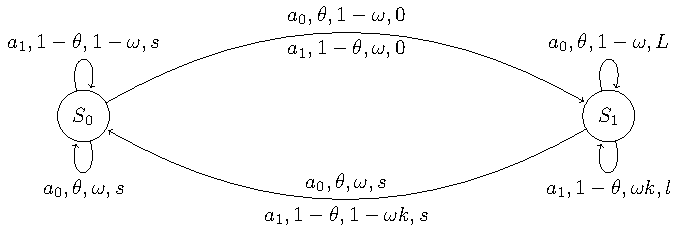
\includegraphics[width=\textwidth]{pictures/chain}
	\caption{Chain problem. On the edges we have (action, action probability, transition probability, reward).}
	\label{fig:chain}
\end{figure}

We use the chain problem as a proof of concept to show the benefits of our algorithm. Using this environment we experimentally validate the ability of REMPS to overcome local minima in the return landscape. \newline The environment in illustrated in \cref{fig:chain}. There are two actions available to the agent denoted with $a_0$ and $a_1$. The policy is very simple and has only one parameter:
\begin{align}
	\pi_\theta(a_0 | s) &=  \theta \; \forall s \in \mathcal{S}, \\
	\pi_\theta(a_1 | s) &=  1 - \theta \; \forall s \in \mathcal{S} \, .
\end{align}
Thus the policy is uniquely defined by the parameter $\theta \in [0,1]$, that is the probability of selecting action $a_0$ and it is the same on all states.
The model has only one parameter, $\omega$, that is the probability of action failure.
Action $a_0$ (forward), if successful, brings the agent to state $s_1$. Action $a_1$ (backward), if successful, brings the agent to state $s_0$.
The agent gets an high reward, $L > 0$, if, starting from state $s_1$ executes successfully action $a_0$. The agent gets a smaller reward $l $, ($0 < l < L$) if it lands in state $s_1$ starting from $s_1$ but executing action $a_1$. Agent gets an even smaller reward, $s$ ($0 < s < l$) when it lands in state $s_0$. The parameter $k$ is not configurable and it has been added to avoid symmetries in the return surface. In the chain problem we are in the ideal case, the model is known, thus we can project the stationary distribution directly.
We initialized the model parameters to $\omega_0$ and the policy parameter to $\theta_0$ such that the initial position in the return landscape is near a local minima. Starting from this position a gradient method should point toward the local maxima, while we empirically demonstrate the ability of our algorithm to reach the pair ($P^*$,$\pi^*$) yielding maximum performance in this environment. The average reward surface as function of the model and policy parameters is illustrated in \cref{fig:chain-rew}. \newline
\begin{figure}[!tb]
\centering
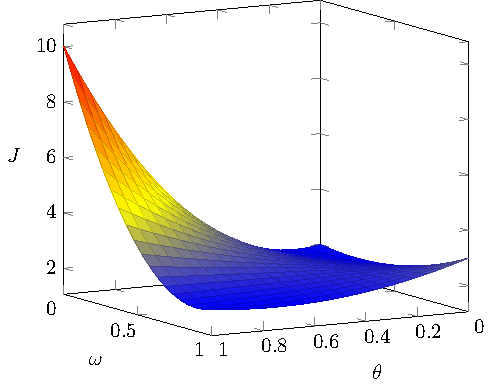
\includegraphics[width=0.8\textwidth]{plots/chain/plot_chain_surface}
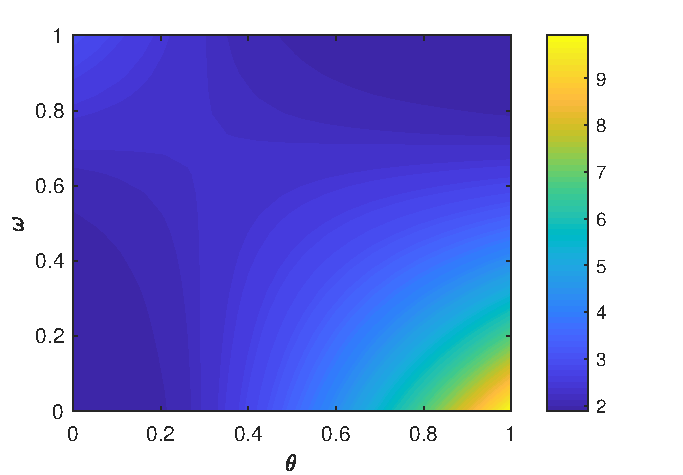
\includegraphics[width=0.8\textwidth]{plots/chain/plot_chain_colormap}
	\caption{Different representations of the average reward surface of the chain experiment as function of model and policy parameters. There is a local maximum in $\theta=0, \omega=1$, a global maximum in $\theta=1, \omega=0$. We start our algorithm near the local minima in $\theta=0.33, \omega=0.66$.}
	\label{fig:chain-rew}
\end{figure}
Table \ref{tab:chain-hyperparameters} summarizes the parameters used in our experiments. \newline
\begin{table}[t]
\centering
\begin{tabular}{ c c}
  \toprule			
  Parameter & Value \\
  \midrule
  $k$ & $0.2$ \\
  $L$ & $10$ \\
  $l$ & $8$ \\
  $s$ & $2$ \\
  $\omega_0$ & $0.8$ \\
  $\theta_0$ & $0.2$ \\
  num of samples & $2 \cdot 10^4$ \\
  num of steps per episode & $5 \cdot 10^2$ \\
\bottomrule
\end{tabular}
\caption{Hyper-parameters used in our chain experiments.} \label{tab:chain-hyperparameters}
\end{table}
We compare the result of our algorithm with G(PO)MDP over model and policy parameters.
It is possible to see that G(PO)MDP, being a gradient method follows the slope of the objective function and it is attracted by the \textit{local} maximum in $\theta=0, \omega=1$. REMPS outperforms G(PO)MDP reaching the \textit{global} maximum in $\theta=1, \omega=0$ after few iterations. We perform different runs varying the $\epsilon$ parameter to show the effect of the parameter. Results are shown in \cref{fig:chain-exp}.

\begin{figure}[!tb]
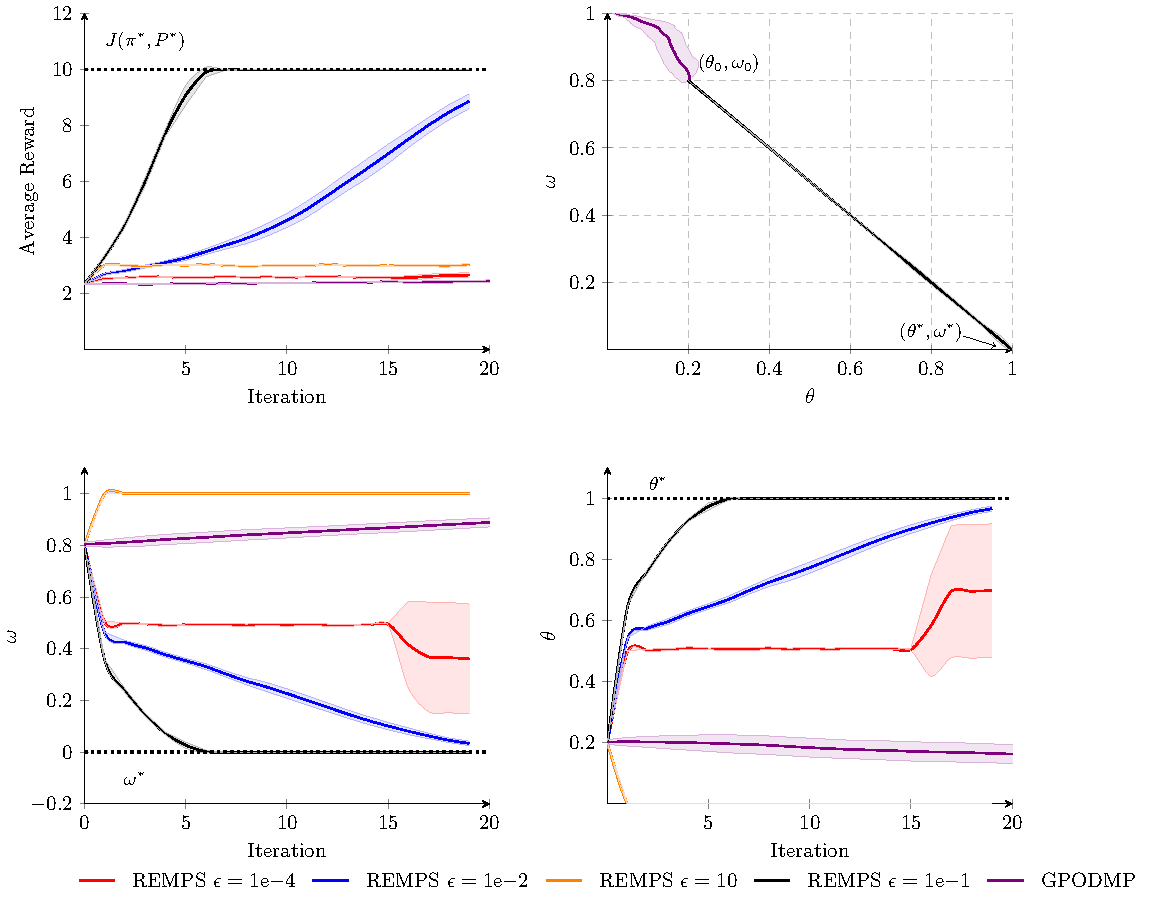
\includegraphics[width=1\textwidth]{plots/chain/plot_chain_all}
\caption{Chain experiment. Top left: average reward of REMPS and GPOMDP. Top right: updates of the model and policy parameter of  GPOMDP and REMPS. Bottom left: shows the updates of the model parameter $\omega$. Bottom right: updates of the policy parameter $\theta$. Shaded areas represent the $95\%$ confidence interval over 10 runs of the algorithm.}
\label{fig:chain-exp}
\end{figure}  

\subsection{Sensitivity to $\epsilon$}
The choice of $\epsilon$ is critical and problem-dependent. A too small $\epsilon$ causes a premature convergence of REMPS to local maximum. A too high $\epsilon$ yields imprecise estimation of the performance of the model-policy target and causes an imprecise projection on the space of possible probability distributions. \cref{fig:jeps} shows the performance of the best model-policy found as function of $\epsilon$. 
We show the value of the primal that is the value of the objective function without any constraint on the policy and model. We can see that the value of the primal is greater than the actual value of the objective after the projection, thus the projection yields a degradation of the performance. The performance degradation is due to the following reason. Moving too far away from the current stationary distribution the primal solution might not be representable using our hypothesis space. Performing a Moment Projection we obtain a  a performance degradation with respect to the original solution.
\begin{figure}[!tb]
\centering
	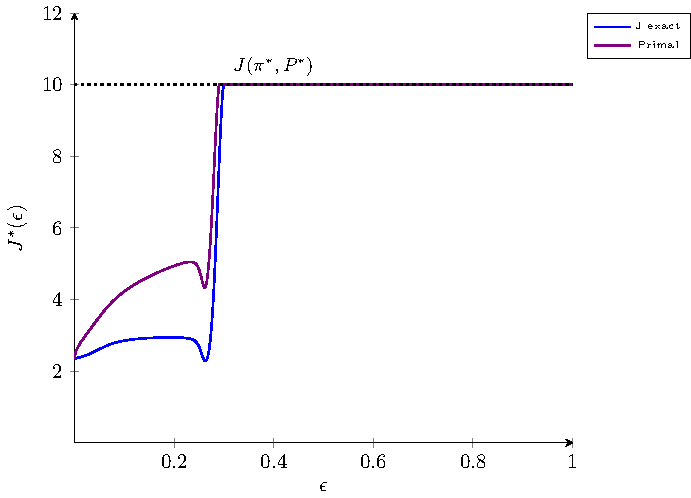
\includegraphics[width=1\textwidth]{plots/chain/plot_j_epsilon}
	\caption{Average reward and primal of the best model-policy couple in the chain experiment as function of $\epsilon$ using the projection of the discounted stationary state distribution.}
	\label{fig:jeps}
\end{figure}
\subsection{Sensitivity to parameter initialization}
REMPS behaves consistently with respect to a random initialization of model and policy parameters. In \cref{fig:chain-random-init} we can see that REMPS updates the model and policy parameters toward the global maximum while GPOMDP updates vary with the initial parameters. In the GPOMDP learning curve it is possible to see clearly the two attractors. REMPS shows a stable behaviour in the case of few model parameters and complex return landscape. 
\begin{figure}[!tb]
\centering
	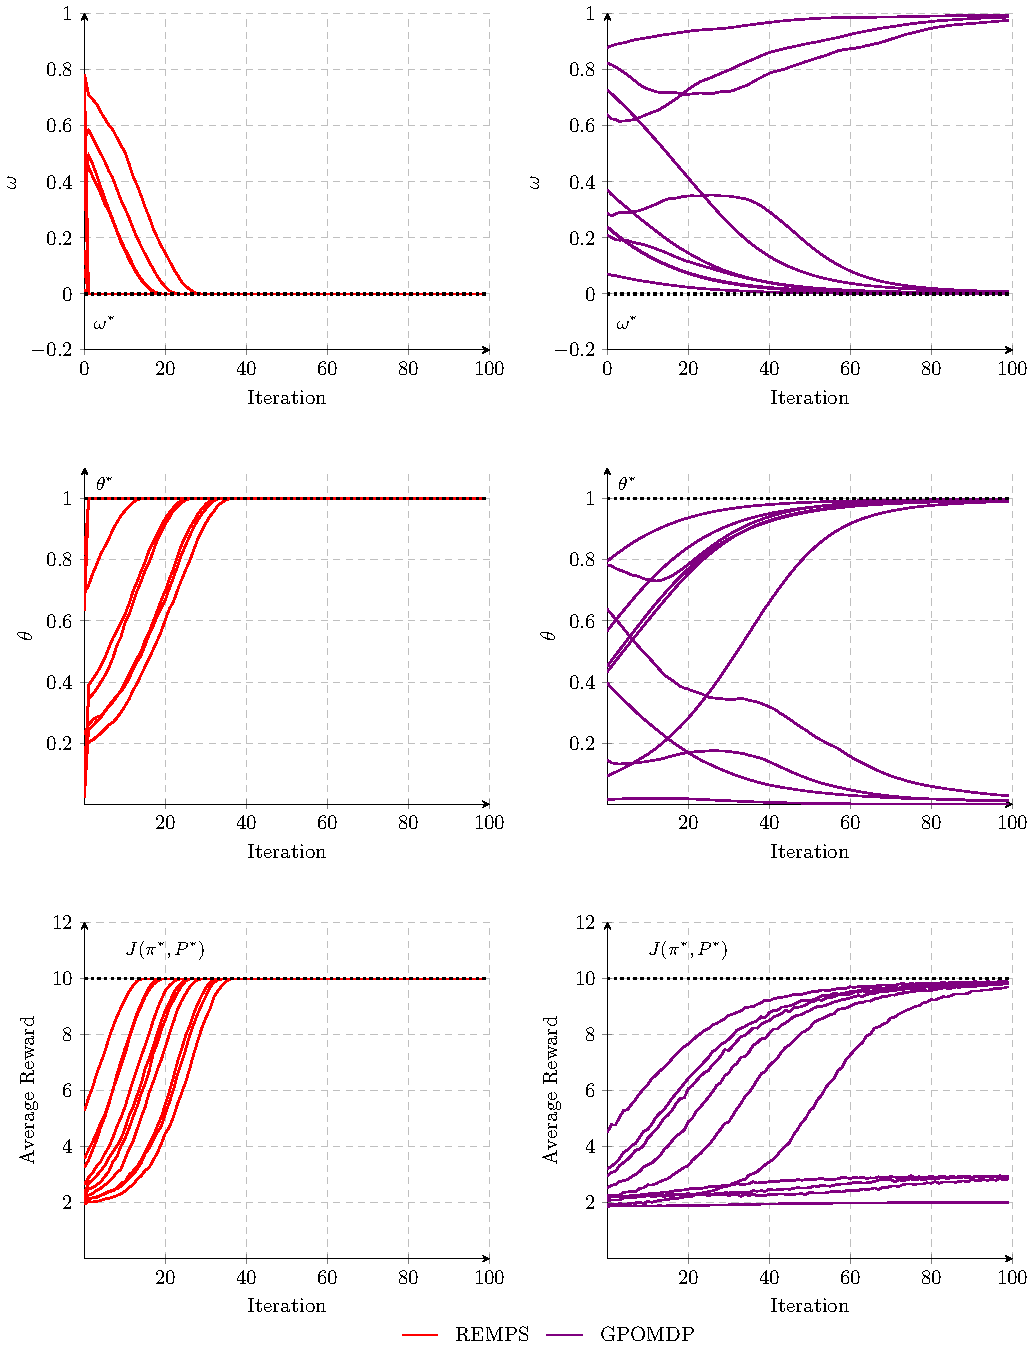
\includegraphics[width=1\textwidth]{plots/chain/plot_random_init}
	\caption{Chain experiment with random initialization of model and policy parameter. Comparison between GPOMDP and REMPS. Top: model parameter. Center: policy parameter. Bottom: average reward.}
	\label{fig:chain-random-init}
\end{figure}
\subsection{Comparison with SPMI}
SPMI is, at the moment of writing, the unique algorithm proposed for CMDPs. We compare in this section the comparison between SMPI and REMPS.
In \cref{fig:chain-spmi} we show the behaviour of the variants of SPMI on the chain experiment. We can easily notice that SPMI requires a huge number of iterations before convergence. While REMPS converges approximately after $10$ iterations, SPMI requires a number of iterations in the order of $10^3$. This is due to the conservative step size of safe approaches. SPMI, SPMI-alt, SPMI-sup and SPI-SMI reach the global maximum while SMI-SPI goes (very slowly) to the local maximum. SMI-SPI is not able to reach the global maximum since it alternates a model improvement step to a policy improvement step considering the two components in a separate manner. \newline
We recall that SPMI is applicable to the chain experiment since this environment has a discrete state space and a discrete action space, while the standard version of this algorithm cannot be applied to the environments presented later in this chapter.
 
\begin{figure}[!tb]
\centering
	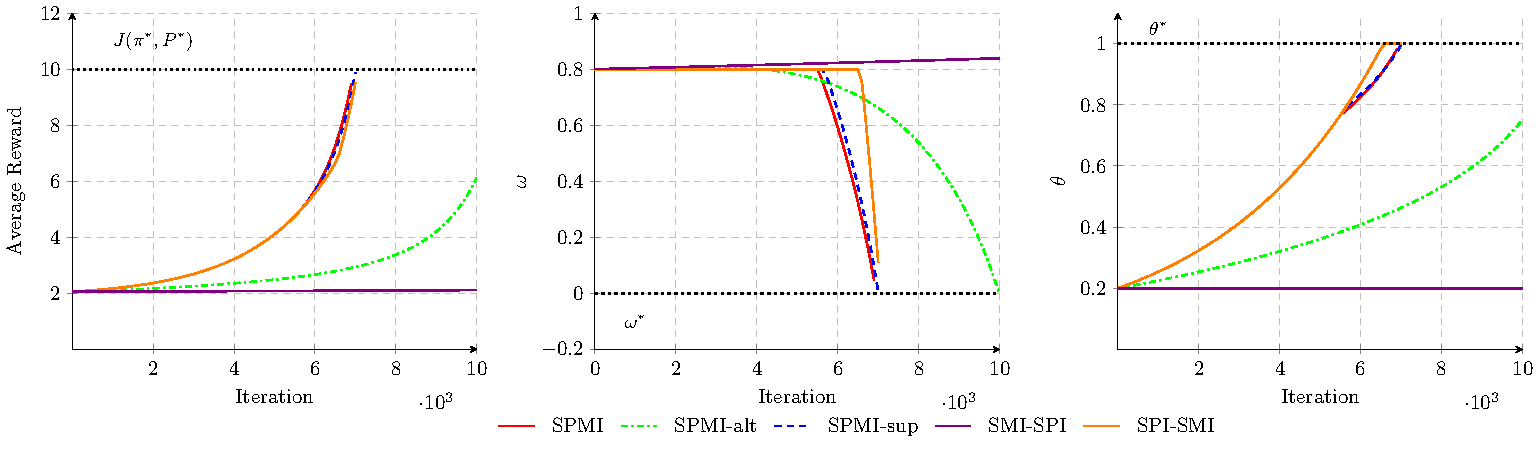
\includegraphics[width=1\textwidth]{plots/chain/plot_spmi}
	\caption{SPMI on the chain experiment. Left: average reward. Center: model parameter. Right: policy parameter.}
	\label{fig:chain-spmi}
\end{figure}

\clearpage

\section{Cart-Pole}\label{sec:cartpole}
The Cart-Pole domain is a standard RL benchmark. The Cart-Pole world consists of a cart that moves along the horizontal axis and a pole that is anchored on the cart. The state space is continuous and it is represented by the $x$ position of the cart, the cart velocity $\dot{x}$, the pole angle $\gamma$ with respect to the vertical, the pole angular velocity $\dot{\gamma}$. The action space is discrete and composed by two actions: left $L$ or right $R$. The model parameter is represented by the force $\omega$ to be applied to the cart, that is the same for both actions. The range of the force is $[0,30]$. The resulting force is $\pm \omega$ depending on the action. We add noise on the resulting action proportional to the force applied and independent noise to each state component. The Cart-Pole environment is represented in \cref{fig:cartpole-env}. \newline
\begin{figure}[!b]
\centering
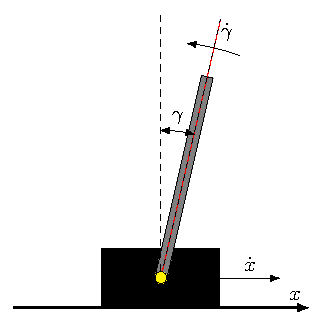
\includegraphics[width = 0.5\textwidth]{plots/cartpole/cartpole_env}
\caption{Cart-Pole environment representation.}
\label{fig:cartpole-env}
\end{figure}
The goal is to keep the pole in the vertical position ($\gamma=0$) as long as possible. The episode ends when the pole reaches a certain angle ($|\gamma| > \bar{\gamma}$) or after a predefined number of steps. We want to encourage smaller forces, to this end we use the following reward function:
$$
R(s,a,s') = 10 - \frac{\omega^2}{20} - 20 \cdot (1 - \cos(\gamma)) .
$$
The first part is a fixed reward for each for each timestep the pole is up and the pole angle is inside the range $[-\bar{\gamma}, +\bar{\gamma}]$. The second part is a penalty proportional to the force. The third part is a penalty proportional the pole angle, it is 0 when the pole is in the vertical position. Ideally the agent should learn to balance the pole with the smaller force possible, keeping it fixed in the vertical position. \newline
\subsection{Results}
We test the performance of REMPS both in the case of an exact model and in the case of an approximated (fitted) model. 
In \cref{fig:cartpole-exp} we show the performance of our algorithm starting from a fixed value of the model parameter, $\omega_0=8$.
\begin{figure}[tb]
\centering
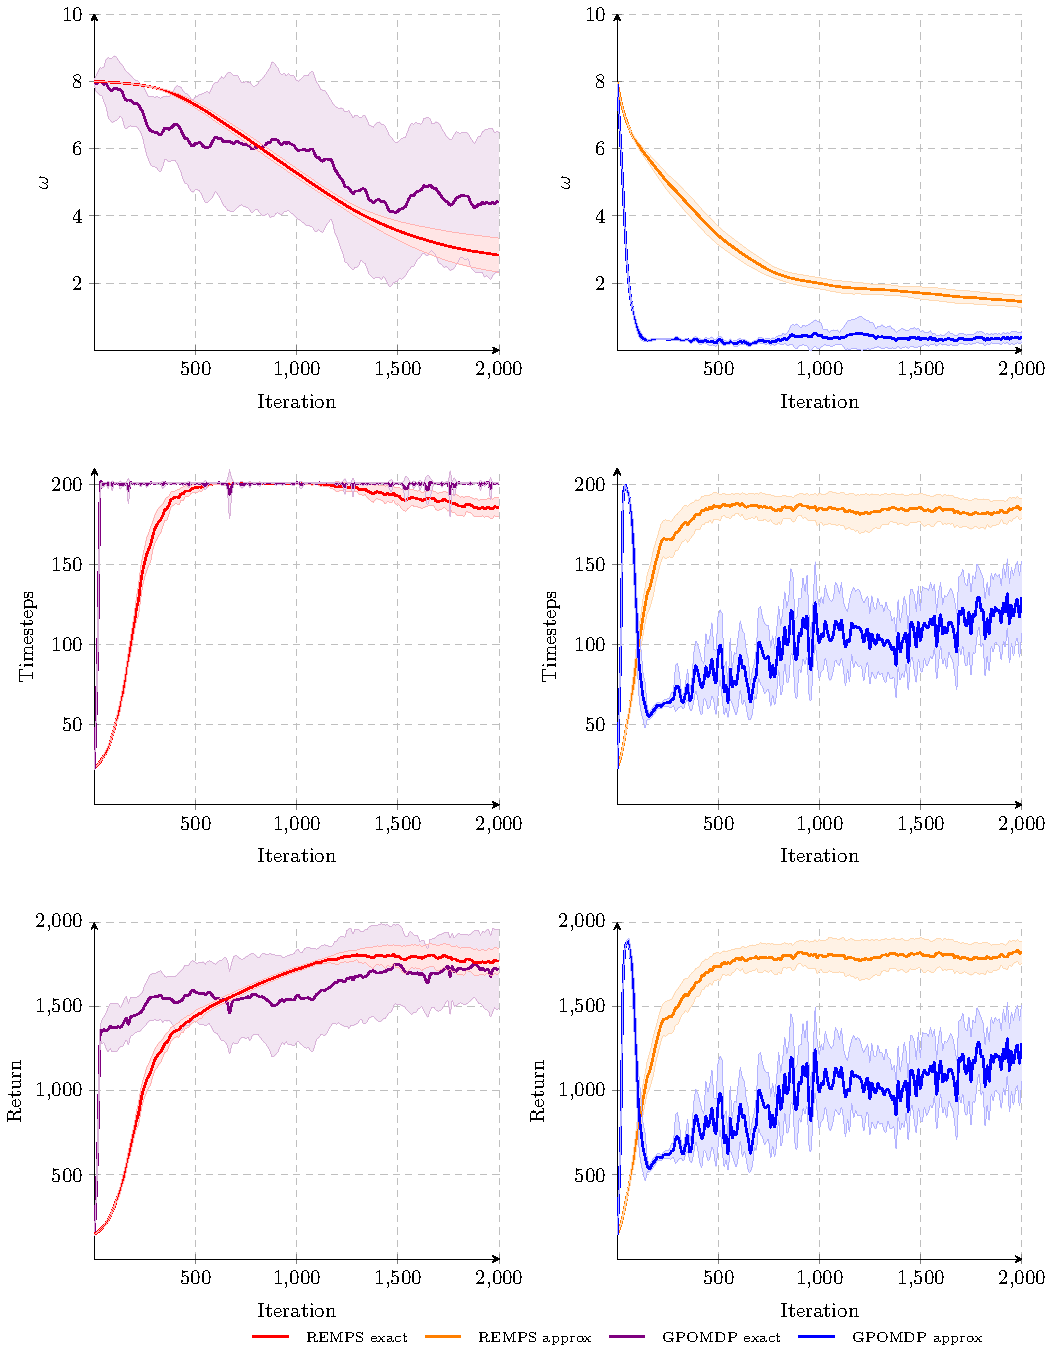
\includegraphics[width = \textwidth]{plots/cartpole/plot_cartpole_experiment}
\caption{Cartpole experiment. Left: results of REMPS and GPOMDP using the exact model. Right: results of REMPS and GPOMDP using the approximated model. Top: model parameter $\omega$. Middle: average timesteps per episode. Bottom: Average return. The shaded area represents the $95\%$ confidence interval over twenty runs of the algorithm.}
\label{fig:cartpole-exp}
\end{figure}
In the exact case, \cref{fig:cartpole-exp} (left), it is possible to see that the model parameter has a decreasing trend in the first iterations, then it converges to a minimum. The timesteps increase and then reach a maximum. The return increases since the agent is less penalized by the force term (since the model parameter is becoming smaller) and it is learning to balance the pole.
In the approximated case, \cref{fig:cartpole-exp} (right),  the cart-pole model is learned by a neural network (NN). The inputs of the NN are the state $s_t$, the action $a_t$ and the model parameter $\omega$. The output neurons represents the mean and the variance of a Gaussian distribution over the state space representing the probability of landing in a given state.
We collect data with a fixed random policy before training. We fitt the dynamic model by maximizing the log-likelihood, obtaining a neural network predicting $P(s' | s, a, \omega)$.
The model learns the effect of the model parameters on the dynamic.
As baseline we use the G(PO)MDP algorithm over the model and policy parameters. Both in the exact version and in the approximated one, REMPS shows a more stable behaviour with respect to G(PO)MDP. In the exact case the two algorithms are comparable, the improvement of REMPS are slower but at the end it outperforms G(PO)MDP with precise selection of the model parameter. \newline
In the approximated case (using the same approximation of the model) REMPS performs better, it is very stable compared to G(PO)MDP. \newline

\begin{table}[!tb]
\centering
\begin{tabular}{ c c}
  \toprule			
  Parameter & Value \\
  \midrule
  Num of samples & $10^5$ \\
  Dual Regularization & 0 \\
  Policy Regularization & 0 \\
  $\epsilon$ & $10^{-3}$ \\
  Policy & Linear with softmax \\
  $\omega_0$ & 8 \\
\bottomrule
\end{tabular}
\caption{Hyper-parameters used in the exact cartpole experiment.} \label{tab:cartpole-hyperparameters-exact}

\vspace*{1 cm}

\begin{tabular}{ c c }
  \toprule			
  Parameter & Value \\
  \midrule
  Num of samples & $5 \cdot 10^4$ \\
  Dual Regularization & $10^{-4}$ \\
  Policy Regularization & $0$ \\
  $\epsilon$ & $10^{-3}$ \\
  Policy & Linear with softmax \\
  $\omega_0$ & 8 \\
\bottomrule
\end{tabular}
\caption{Hyper-parameters used in the approximated cartpole experiment.} \label{tab:cartpole-hyperparameters-approx}

\end{table}

%\begin{table}[!t]
%\centering
%\begin{tabular}{ c c }
%  \toprule			
%  Parameter & Value \\
%  \midrule
%  Num of samples & $5 \cdot 10^4$ \\
%  Dual Regularization & $10^{-4}$ \\
%  Policy Regularization & $0$ \\
%  $\epsilon$ & $10^{-3}$ \\
%  Policy & Linear with softmax \\
%  $\omega_0$ & 8 \\
%\bottomrule
%\end{tabular}
%\caption{Hyper-parameters used in the approximated cartpole experiment.} \label{tab:cartpole-hyperparameters-approx}
%\end{table}


%\paragraph{Random Initialization} In \cref{fig:cartpole-random-init} we compare the approximated versions of REMPS and GPOMDP on the cart-pole experiment with random initialization of the model parameter. For a wide range of the initial model parameter REMPS converges to the optimal parameter. GPOMDP shows an unstable, oscillating behaviour.
%
%
%\begin{figure}[!tb]
%\centering
%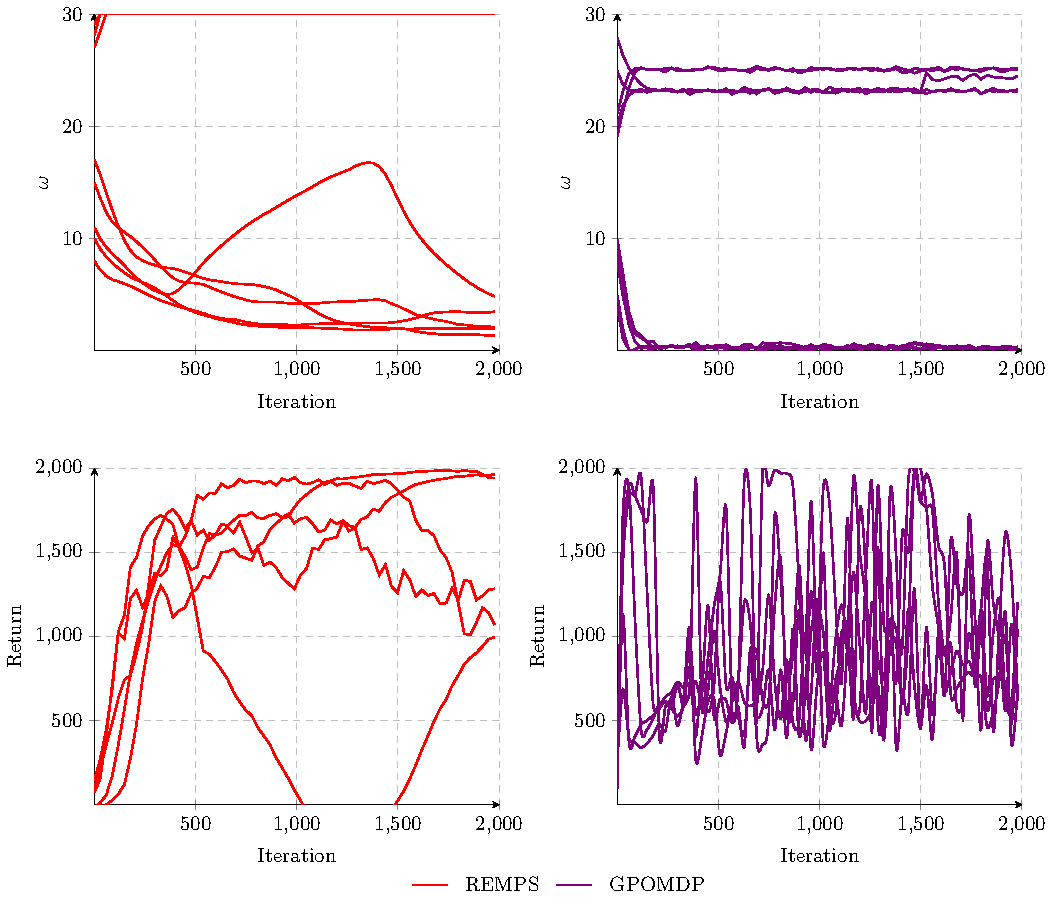
\includegraphics[width = \textwidth]{plots/cartpole/plot-random-init}
%\caption{Cartpole experiment with random initialization of the model parameter. Left: REMPS, right: GPOMDP.}
%\label{fig:cartpole-random-init}
%\end{figure}

\clearpage

\section{Autonomous Driving and Configuration with TORCS}\label{sec:torcs}
The Open Racing Car Simulator \citep{TORCS}, TORCS, is a car racing simulation, which allows to simulate driving races. It is a complete 3D racing simulator offering a complete set of sensors and controls. TORCS has been used as RL environments in \citep{torcs-1, torcs-2, torcs-3, torcs-4} and many others. \newline
We modified the source code of TORCS adding the possibility to configure the car parameters following the "Car Setup Competition".\footnote{https://sourceforge.net/projects/cig} 
The goal of this experiment is to show the benefits of the environment configuration in the context of autonomous driving. 
\subsection{Environment Description}
The state space of the TORCS environment is composed by $29$ dimensions, $\mathcal{S} \subseteq \mathbb{R}^{29}$. The action space is composed by 2 dimensions, $\mathcal{A} \subseteq \mathbb{R}^2$. The first dimension of the action space is the acceleration/brake action, while the second dimension is the steering angle. The configuration space is very large, so we considered only a subset in our experiments.
All configuration parameters are normalized in the range $[0,1]$.
The state space space is summarized in \cref{tab:torcs-state} and the configuration parameters in \cref{tab:torcs-conf}. 
\begin{table}[tb]
\centering
\begin{tabular}{ c | l }
  \toprule			
  Parameter & Description \\
  \midrule
  angle & Angle between the car direction \\
  &  and the direction of the track axis. \\
  rpm & Number of rotation per minute of the car engine. \\
  speedX & Speed of the car along the longitudinal axis of the car. \\
  speedY & Speed of the car along the transverse axis of the car. \\
  speedZ & Speed of the car along the Z axis of the car.\\
  track & Vector of 19 range finder sensors: each sensors returns the \\
  & distance between the track edge and the car within \\
  & a range of 200 meters. \\
  trackPos & Distance between the car and the track axis. \\
  wheelSpinVel & Vector of 4 sensors representing the rotation speed of wheels. \\
\bottomrule
\end{tabular}
\caption{State space of the TORCS experiment.} \label{tab:torcs-state}
\end{table}
\begin{table}[tb]
\centering
\begin{tabular}{ c | l }
  \toprule			
  Parameter & Description \\
  \midrule
  Rear Wing & Angle of the rear wing. \\
  Front Wing & Angle of the front wing. \\
 Front-Rear Brake Repartion & Repartition of the brake between the front and rear. \\
   Front Anti-Roll Bar & Front Spring. \\
  Rear Anti-Roll Bar & Rear Spring.\\
  Front Left-Right Brake & Brake disk diameter of the front wheels.\\
  Rear Left-Right Brake & Brake disk diameter of the rear wheels. \\
\bottomrule
\end{tabular}
\caption{Configuration space of the TORCS experiment.} \label{tab:torcs-conf}
\end{table}
We defined the reward function in the following way:
\begin{equation}
	R(s,a,s') = \text{speedX}' \cdot  \cos ( \text{angle}' ),
\end{equation}
where $\text{speedX}'$ is the velocity on the longitudinal direction of the car in state $s'$ and $\text{angle}'$ is the angle between the car direction and the direction of the track axis.  We give a penalty of $1000$ if the agent runs backward, if it goes out of track or if the progress in the race is too low. The rationale behind this reward is to encourage the agent to go at high speed and to stay centered with respect to the track. \newline
The policy we used in our experiments is a Gaussian Policy parameterized by a fully connected neural network:
\begin{equation}
	\pi(a|s) = \mathcal{N}(\boldsymbol{\phi_m}(s), \boldsymbol{\phi_v}),
\end{equation}
where the mean $\boldsymbol{\phi_m}(s)$ is a non-linear function of the current state $s$ and the variance $\boldsymbol{\phi_v}$ it is independent from the current state. \newline
In the projection phase of REMPS we can only perform a disjoint projection of the policy and model (see \cref{sec:disjproj}) since the state and action spaces are continuous.
\subsection{Results}
In the first phase of our experiments we run a random policy in order to collect the dataset for model fitting. We fitted the model with a neural network using a predefined number of iterations as in \cref{sec:cartpole}. During the actual training phase we used the model network to approximate the system dynamics and we optimized the policy and the environment configuration.
A comparison between the results obtained learning only the policy (REPS) and the results obtained learning the policy and the environment configuration (REMPS) are given in \cref{fig:torcs}. Configuring the environment yields a performance boosting even in an environment with complex dynamic and even starting with a random policy, where the effect of the configuration is limited. We highlight the fact that we learn the model once using a fixed, random policy, while we could alternate model-policy optimization and model fitting for a more precise estimation. 


\begin{figure}[!tb]
\centering
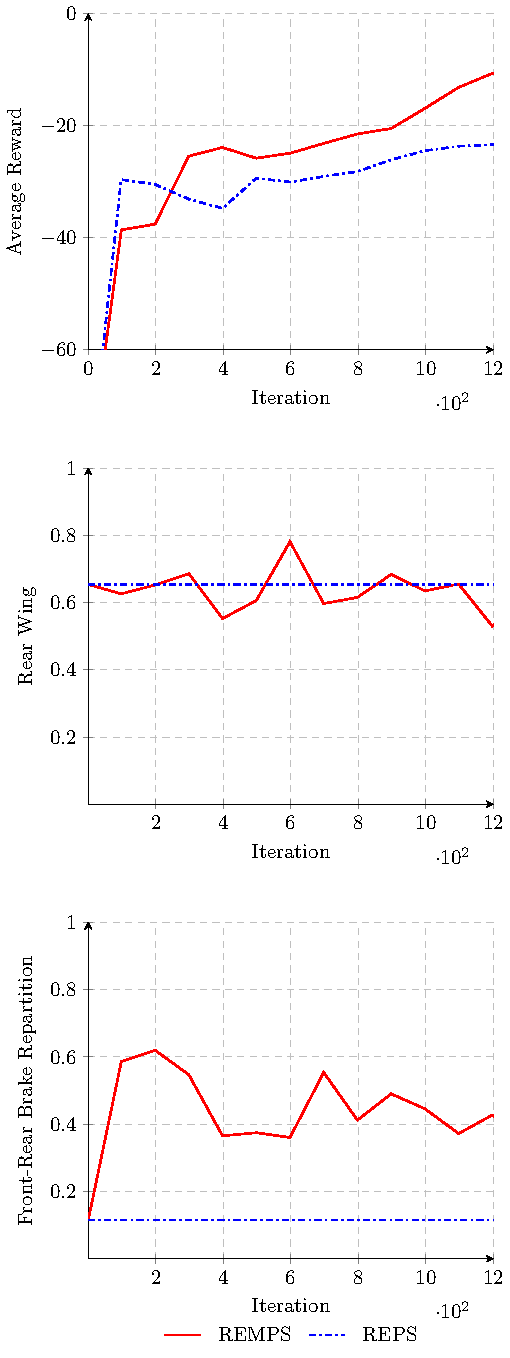
\includegraphics[width = 0.6\textwidth]{plots/torcs/plot_torcs}
\caption{TORCS experiment. Comparison between policy learning and policy-configuration learning. Learning the configuration yields a performance improvement. Top: Average reward. Middle: Rear wing angle. Bottom: Front-Rear Brake repartition.}
\label{fig:torcs}
\end{figure}
\chapter{Discussion and Conclusions}
\label{capitolo7}
\thispagestyle{empty}
\vspace{0.5cm}

\noindent In this chapter, we discuss the main contribution of this thesis, and we propose some possible future extensions and refinement of the approaches presented in this work. 
The first contribution of this document is a new algorithm, namely \textbf{REMPS}, able to solve the model-policy learning problem in the context of CMDPs. 
REMPS is an extension of REPS \citep{reps} that considers also the model optimization. Along with REMPS we present three types of policy and model projection strategies in order to deal with limited representation power. 
REMPS is able to work with continuous state and action spaces, moreover it does not require the knowledge of the full transition model, requiring only an approximation.
\paragraph{}
We presented a theoretical study of the property of the algorithm, providing a lower bound to the difference between the performance of the solution found using an infinite number of sample and infinite representation power and the solution using a finite number of samples and finite representation power. We showed that this bound depends on the number of samples, on the representation power of the model and policy spaces and on the value of the KL--constraint $\epsilon$. \newline
\paragraph{}
Along with a theoretical study of the algorithm, we presented also an empirical evaluation. We tested our algorithm on three domains. The first domain (chain problem) is a proof of concept showing the ability of REMPS to overcome local minima. The second domain (cart-pole) is a standard RL benchmark with continuous action space, discrete action space. We used cart-pole to test the performances in both the exact model and in the approximated model scenarios. The last experiment is a complex experiment of autonomous driving and configuration using the TORCS environment.
In our experiments we showed the benefits of model configuration and the benefits of using an information theoretical approach with respect to a gradient method such as G(PO)MDP.
\paragraph{}
We outline some possible extensions and research directions.
\paragraph{Adaptive $\epsilon$}
The $\epsilon$ parameter in the KL constraint is critical since it is responsible for the magnitude of the update. A high value of $\epsilon$ results in too large model-policy updates, while a too small $\epsilon$ results in no updates at all. An optimal value for $\epsilon$ can be found using heuristics or using a principled way, optimizing some utility function.
\paragraph{Other divergences}
REMPS (and REPS) algorithm is based on the KL divergence. The usage of this kind of distance is justified by the closed form solution of the learning problem. However the KL distance has some problems. The first problem is that it is not symmetric, so after the model-policy projection we have no clue on the distance from the projected model and policy to the ones used for sampling. Moreover the use of KL distance requires the policy to be stochastic, since the KL between two deterministic policy is $0$ or $\infty$. 
An interesting extension of our algorithm could use different types of distance, i.e. Rényi divergence, Hellinger or Weisserstein. We highlight the fact that using the Total Variation distance it is not possible to solve the REMPS optimization problem in closed form.
\paragraph{Policy Space Identification}
The presented approach to the CMDP learning problem is a joint approach, in which the supervisor and the agent are the same entity. In a realistic case the two entity can be different, i.e. an F1 pilot and a mechanical engineer. In these cases it can be beneficial to split the policy learning and the model learning. The agent should be freely allowed to learn using some strategy, the supervisor should study the agent behaviour proposing for each episode the best (according to some utility measure) environment configuration. In order to do this the supervisor should know the agent's policy space. However, in realistic cases the policy can be unknown. In these scenarios the supervisor should identify the policy space of the agent and perform optimizations using this approximation.
\paragraph{Finite--Time Analysis}
In our theoretical analysis we derived a bound valid for a single step of REMPS. An interesting theoretical extension would be an analysis for multiple steps of REMPS obtaining a bound on $J_{d^{(T)}} - J_{\widetilde{d}^{(T)}}$, where $d^{(T)}$ is the distribution obtained using infinite samples after T step of optimization and $\widetilde{d}^{(T)}$ is the solution obtained with $N$ samples with limited capacity on the model and policy selection.

\cleardoublepage
% ---- Bibliography ----
\addcontentsline{toc}{chapter}{Bibliography}
\bibliographystyle{mydinat}
\bibliography{bibl_tesi}

%\nocite{*}

\appendix

\pagestyle{fancy} 
\fancyfoot{}                                               
\renewcommand{\chaptermark}[1]{\markboth{\appendixname\ \thechapter.\ #1}{}} 
\renewcommand{\sectionmark}[1]{\markright{\thesection.\ #1}}         
\fancyhead[LE,RO]{\bfseries\thepage}    
                                        
\fancyhead[RE]{\bfseries\leftmark}    
\fancyhead[LO]{\bfseries\rightmark}     
\renewcommand{\headrulewidth}{0.3pt} 

\chapter{Proof of Linear Programming Formulation}
\label{LPproof}
\thispagestyle{empty}

\noindent This appendix provides the proof of Theorem \ref{lpth} that we report here for completeness:
\begin{align*}
	\underset{v}{\text{minimize}} & \; \sum_{s \in \mathcal{S}} \mu(s) v(s) \\
	\text{subject to} &  \; v(s) \geq r(s,a) + \sum_{s' \in \mathcal{S}} P(s' \mid s,a) v(s') \, , \forall a \in \mathcal{A} \, .
\end{align*} 

\begin{theorem*}[Linear Programming Solution]
$v^*$ is the solution of the above linear program.
\end{theorem*}

\begin{proof}
	Let $T^*$ be the Bellman optimality operator, then the above LP can be rewritten as:
	\begin{align*}
	\underset{v}{\text{minimize}} & \; \mu^T v \\
	\text{subject to} &  \; v \geq T^* (v) \, .
\end{align*} 
Using the \textit{monotonicity property} if $v \geq T^*(v)$, then $T^*(v) \geq T^*(T^*(v))$, and by applying infinite times the operator we obtain: $v \geq T^{* \infty} (v) = v^*$. Any feasible solution of the LP must satisfy $v \geq T^* (v)$, thus it must satisfy  $v \geq v^*$. Hence, assuming all entries $\mu$ are positive, $v^*$ is the optimal solution to the LP.
\end{proof}
\chapter{Gradient Methods for CMDP}
\label{gradient_cmdp}
\thispagestyle{empty}
In this section we provide the straightforward extension of REINFORCE and G(PO)MDP gradient estimation optimizing the policy and the configuration parameters.
\section{REINFORCE}
Let us start by stating the expression of the gradient of the expected return with respect to a parametric transition model differentiable in its parameters $\boldsymbol{\omega}$.
\begin{theorem}[P-Gradient Theorem, from \citep{cmdp}] Let $P_\omega$ be a class of parametric stochastic transition models differentiable in $\boldsymbol{\omega}$, $\pi$ be the current policy, the gradient of the expected return with respect to $\boldsymbol{\omega}$ is given by:
$$
\nabla_{\boldsymbol{\omega}}J^{P,\pi} = \int_{\mathcal{S}}\int_{\mathcal{A}} d^{P,\pi}(s,a) \int_{\mathcal{S}} \nabla_{\boldsymbol{\omega}}P_{\boldsymbol{\omega}}(s'|s,a)u^{P,\pi}(s,a,s') \mathrm{d}s' \mathrm{d}a \mathrm{d}s
$$
	
\end{theorem}

We can now derive in a straightforward manner the REINFORCE estimator for model learning:
\begin{equation}
\widehat{\nabla_{\boldsymbol{\omega}} J^{P,\pi}}_{RF} = \langle \left(\sum_{k=0}^H \nabla_{\bm{\omega}} \log P_{\boldsymbol{\omega}}(s_{k+1} |s_k, a_k) \right) \left( \sum_{k=0}^H \gamma^k R(s_k,a_k, s_{k+1}) \right) \rangle_N \, ,
\end{equation}
where $\langle \cdot \rangle_N$ denotes the empirical average over a batch size of dimension $N$.

\section{G(PO)MDP}
\label{gpomdp_cmdp}
In order to derive the G(PO)MDP estimator for model learning we start from a trajectory based perspective:

$$
J^{P,\pi} = \int p_{\boldsymbol{\theta},\boldsymbol{\omega}}(\tau)G(\tau) \mathrm{d}\tau,
$$
where $p_{\boldsymbol{\theta},\boldsymbol{\omega}}(\tau)$ is the probability of the trajectory $\tau$ under the distribution induced by the parameters $\boldsymbol{\theta},\boldsymbol{\omega}$ and $G(\tau)$ is the return of the trajectory $\tau$.
Using the log-trick and taking the derivative with respect to the model parameters we obtain:
\begin{align}
	\nabla_{\boldsymbol{\omega}}J^{P,\pi} &= \int p_{\boldsymbol{\theta},\boldsymbol{\omega}}(\tau) \nabla_{\boldsymbol{\omega}}\log p(\tau) G(\tau) \mathrm{d}\tau \\
	&= \int p_{\boldsymbol{\theta},\boldsymbol{\omega}}(\tau) \left(\sum_{k=0}^{H} \log P_{\boldsymbol{\omega}}(s_{k+1} | s_k, a_k)  \right) G(\tau) .
\end{align}
Now we are exactly in the G(PO)MDP settings and we can use the following approximation of the gradient:
\begin{equation}
\widehat{\nabla_{\boldsymbol{\omega}} J^{P\pi}}_{G(PO)MDP} = \langle \sum_{l=0}^H \left( \sum_{k=l}^H \nabla_{\bm{\omega}} \log P_{\boldsymbol{\omega}}(s_{k+1} | s_k, a_k) \right) \left( \gamma^l R(s_l,a_l, s_{l+1}) \right) \rangle_N \, ,
\end{equation}
where $\langle \cdot \rangle_N$ denotes the empirical average over a batch size of dimension $N$.
\chapter{REMPS derivation}
\label{sec:remps_deriv}
\thispagestyle{empty}

\noindent This appendix provides the derivation of the REMPS solution.
We report here the formulation of the REMPS problem. For the sake of brevity we use $\mathcal{X} = \mathcal{S} \times \mathcal{A} \times \mathcal{S}$ and $(s,a,s') = x \in \mathcal{X}$, moreover we indicate with $d(\cdot)$ the optimized distribution and with $d^{P,\pi}(\cdot)$ the sampling distribution.
\begin{align}
	\underset{d}{\text{maximize}} & \; \int_\mathcal{X}d(x)R(x) \\
	\text{subject to} &  \; \int_\mathcal{X}d(x) \log \frac{d(x)}{d^{P,\pi}(x)} \mathrm{d}x \leq \epsilon \\
	& \int_\mathcal{X} d(x) \mathrm{d}x = 1 \ \, .
\end{align} 

We solve the problem with Lagrangian multipliers. We denote with $\eta$ the langrangian multiplier associated with the KL constraint and with $\lambda$ the multiplier associated with the constraint of being a valid distribution.
\begin{align}
	\mathcal{L}(d(\cdot), \eta, \lambda) = &\int_\mathcal{X} d(x)R(x) \mathrm{d}x +\\ &+ \eta \left( \epsilon - \int_\mathcal{X} d'(x) \log \frac{d(x)}{d^{P,\pi}(x)} \mathrm{d}x \right) +\\ &+ \lambda \left(1 - \int_\mathcal{X} d(x) \mathrm{d}x \right) \, .
	\label{eq:lagrangian}
\end{align}
Observe that $\frac{\partial}{\partial f(x_0)} \int f(x) g(x) dx = g(x_0)$. So we take the derivative with respect to $d(x)$ to get:
\begin{equation}
	R(x) - \eta \log \frac{d(x)}{d^{P,\pi}(x)} + \eta - \lambda = 0 \, ,
\end{equation}
from which we get, solving for $d(x)$:
\begin{equation}
	d(x) = d^{P,\pi}(x) \exp \left(\frac{R(x)}{\eta} \right) \exp \left( 1 - \frac{\lambda}{\eta} \right) \, .
	\label{eq:remps-pol}
\end{equation}
By enforcing the constraint that $d$ should be a valid distribution we obtain:
\begin{equation}
	d(x) = \frac{d^{P,\pi}(x) \exp \left(\frac{R(x)}{\eta} \right)}{\int_\mathcal{X} d^{P,\pi}(x) \exp \left( \frac{R(x)}{\eta} \right) \mathrm{d}x} \, .
\end{equation}

Substituting into the Lagrangian function (\ref{eq:lagrangian}), we obtain the dual function:
\begin{align}
	g(\eta, \lambda) &= -\eta + \eta\epsilon + \lambda \\
	&= \eta \log \left( \int_\mathcal{X} d^{P,\pi}(x) \exp \left(\epsilon + \frac{R(x)}{\eta} \right)\mathrm{d}x \right) \, .
\end{align}

From (\ref{eq:remps-pol}) we extract the policy and model inducing the distribution $d$. We return to the original formulation for the sake of clarity.
\begin{align}
	\pi'(a | s) &= \frac{\int_\mathcal{S}d(s,a,s') \mathrm{d}s'}{\int_\mathcal{A}\int_\mathcal{S}d(s,a,s') \mathrm{d}s' \mathrm{d}a} \\
	&= \frac{\pi(a | s) \int_\mathcal{S} P(s' | s,a) \exp \left( \epsilon + \frac{R(x)}{\eta} \right) \mathrm{d}s'}{\int_\mathcal{A} \pi(a | s) \int_\mathcal{S} P(s'|s,a) \exp \left( \epsilon + \frac{R(x)}{\eta} \right) \mathrm{d}s' \mathrm{d}a}, \\
	P'(s' | a, s) &= \frac{d(s,a,s')}{\int_\mathcal{S}d(s,a,s') \mathrm{d}s'} \\
	&= \frac{P(s' | s,a) \exp \left( \epsilon + \frac{R(x)}{\eta} \right)}{\int_\mathcal{S} P(s' | s,a) \exp \left( \epsilon + \frac{R(x)}{\eta} \right) \mathrm{d}s'} \; .
\end{align}


\end{document}







